\newcommand{\comments}[1]{}
\documentclass[twoside,12pt,letterpaper]{report}
\tolerance=1000  
\hbadness=10000  
\raggedbottom




% Paquetes para manejar graficos
\usepackage{epsf}
\usepackage[pdftex]{graphicx}
\usepackage{epsfig}
% Simbolos matematicos
\usepackage{latexsym,amssymb}
% Paquetes para presentar una tesis decente.
\usepackage{setspace,cite} % Doble espacio para texto, espacio singular para
                           % los caption y pie de pagina

% Paquetes no utilizados para citas
%\usepackage{mcite} 
%\usepackage{draft} 

\usepackage{wrapfig}
\usepackage{alltt}
\usepackage{url}

\usepackage[toc,style=altlist,nonumberlist]{glossaries}
%\renewcommand{\glossaryname}{Lista de abreviaturas y símbolos}

% Acentos 
\usepackage[spanish,activeacute]{babel}
\usepackage[spanish]{translator}
\usepackage[utf8]{inputenc}
\usepackage{color, colortbl}
\usepackage{multirow}
\usepackage{subfig}
\usepackage[OT1]{fontenc}
\usepackage{tocbibind}
\usepackage{anysize}
\usepackage{listings} 
\usepackage[table]{xcolor}
% Para poder tener texto asiatico
%\usepackage{CJK}


% Opciones para los glosarios
%\usepackage[style=altlist,toc,numberline,acronym]{glossaries}
\usepackage{url}
\usepackage{amsthm}
\usepackage{amsmath}
\usepackage{fancyhdr} % Necesario para los encabezados
\usepackage{fancyvrb}
\usepackage{makeidx} % En caso de necesitar indices.
\makeindex  % Necesitado para los indices

% Definiciones para definicions, teoremas y lemas
\theoremstyle{definition} \newtheorem{definicion}{Definici\'{o}n}
\theoremstyle{plain} \newtheorem{teorema}{Teorema}
\theoremstyle{plain} \newtheorem{lema}{Lema}

% Para la creacion de los pdfs
\usepackage{hyperref}

% Para resolver el lio del Unicode para la informacion de los PDFs
% En pdftitle coloca el nombre de su proyecto de grado/pasantia.
% En pdfauthor coloca su nombre.
\hypersetup{
    pdftitle = {SISTEMA DE APRENDIZAJE DE CONTROLADORES DIFUSOS PARA CONDUCCIÓN AUTOMÁTICA DE VEHÍCULOS},
    pdfauthor={Alejandro Do Nascimiento Mora},
    colorlinks,
    citecolor=black,
    filecolor=black,
    linkcolor=black,
    urlcolor=black,
}

% Crea el glosario
\makeglossaries

% Incluye el glosario
\newacronym{CSIC}{CSIC}{Consejo Superior de Investigaciones Científicas}
\newacronym{CAR}{CAR}{Centro de Automática y Robótica}
\newacronym{ITS}{ITS}{Sistemas Inteligentes de Transporte (\textit{Intelligent Transportation Systems})}
\newacronym{IAI}{IAI}{Instituto de Automática Industrial}
\newacronym{UPM}{UPM}{Universidad Politécnica de Madrid}
\newacronym{ORBEX}{ORBEX}{Ordenador Borroso Experimental}
\newacronym{ZOCO}{ZOCO}{Zona de Conducción}
\newacronym{DGPS}{DGPS}{Differential Global Positioning System}
\newacronym{GPS}{GPS}{Global Positioning System}
\newacronym{CAN}{CAN}{Control Area Network}
\newacronym{WLAN}{WLAN}{Wireless Area Network}
\newacronym{ABS}{ABS}{Antilock Breaking System}
\newacronym{IMU}{IMU}{Inertial Measurement Unit}
\newacronym{TORCS}{TORCS}{The Open Racing Car Simulator} 
\newacronym{MAE}{MAE}{ error absoluto medio (\textit{Mean Absolute Error})} 
\newacronym{GPL}{GPL}{Licencia Pública General (\textit{General Public License}}
\newglossaryentry{error}
{
  name={\ensuremath{\varepsilon_v(i)}},
  description={Error de velocidad en el instante de tiempo $i$},
  sort=1error
}
\newglossaryentry{Cte}
{
  name={\ensuremath{Cte}},
  description={Constante de normalización},
  sort=constante
}
\newglossaryentry{mu_{i}(t-1)}
{
  name={\ensuremath{mu_{i}(t-1)}},
  description={Grado de activación del singleton $i$ en el instante de tiempo (t-1)},
  sort=1grado
}
\newglossaryentry{s(t)}
{
  name={\ensuremath{s(t)}},
  description={Singleton en el instante $t$},
  sort=singleton
}
\newglossaryentry{P(i)}
{
  name={\ensuremath{P(i)}},
  description={Perfil de velocidad durante el instante de tiempo $i$},
  sort=perfil
}
\newglossaryentry{V(i)}
{
  name={\ensuremath{V(i)}},
  description={Velocidad del velocidad durante el instante de tiempo $i$},
  sort=velocidad
}
\newglossaryentry{a(i)}
{
  name={\ensuremath{a(i)}},
  description={Aceleración del velocidad durante el instante de tiempo $i$},
  sort=aceleracion
}
\newglossaryentry{dedt}
{
  name={\ensuremath{\frac{d(\varepsilon_v(i))}{d(t)}}},
  description={Derivada del error de velocidad con respecto al tiempo},
  sort=1derivada
}
\newglossaryentry{a_c}
{
  name={\ensuremath{a_c}},
  description={Aceleración de confort},
  sort=aceleracionc
}
\newglossaryentry{t(i)}
{
  name={\ensuremath{t(i)}},
  description={tiempo en el instante $i$},
  sort=t
}
\newglossaryentry{summod}
{
  name={\ensuremath{\sum_{x= i-10}^{i}\mid\varepsilon_v(x)\mid}},
  description={Suma del modulo del error de velocidad de los últimos diez instantes de tiempo},
  sort=1sumatoria
}

\newglossaryentry{integrall}
{
  name={\ensuremath{\int_{i-10}^{i}\varepsilon_v(i)}},
  description={Integral del error de velocidad durante los últimos diez instantes de tiempo},
  sort=1integral
}
\newglossaryentry{Microsoft Visual C++ Express}
{	
	name={Microsoft Visual C++ Express},
    description={Entorno de desarrollo integrado (IDE) gratuito desarrollado por Microsoft para lenguajes de programación C, C++ y C++/CLI} 
}
\newglossaryentry{Microsoft Windows XP}
{	
	name={Microsoft Windows XP},
    description={Versión del sistema operativo Microsoft Windows} 
}
\newglossaryentry{C++}
{
	name={C++},
    description={Lenguaje de programación diseñado con la intención de extender al lenguaje de programación C con mecanismos que permitan la manipulación de objetos}   
}
\newglossaryentry{singletons}
{
	name={Singletons},
    description={Conjunto con un único elemento}   
}
\newglossaryentry{Open Source}
{
	name={Open Source},
    description={Código abierto, es el término con el que se conoce al software distribuido y desarrollado libremente}
}

\newglossaryentry{Linux}
{
	name={Linux},
    description={Núcleo libre de sistema operativo basado en Unix}
}

\newglossaryentry{x86}
{
	name={x86},
    description={Nombre dado al grupo de microprocesadores de la familia de Intel y a la arquitectura que comparten estos procesadores}
}

\newglossaryentry{AMD64}
{
	name={AMD64},
    description={Arquitectura basada en la extensión del conjunto de instrucciones x86 para manejar direcciones de 64 bits}
}

\newglossaryentry{PPC}
{	
	name={PPC},
    description={Sistema operativo Linux que posee un kernel nativo PPC}
}

\newglossaryentry{FreeBSD}
{	
	name={FreeBSD},
    description={Sistema operativo libre basado en las CPU de arquitectura Intel}
}

\newglossaryentry{MacOSX}
{
	name={MacOSX},
    description={Sistema operativo desarrollado y comercializado por Apple Inc.}
}

\newglossaryentry{Windows}
{
	name={Windows},
    description={familia de sistemas operativos desarrollados por Microsoft}
}
\addto\captionsspanish{%
\def\glossaryname{Lista de abreviaturas y símbolos}%
}
% Para crear la hoja escaneada de las firmas
\usepackage[absolute]{textpos}

% Pone los nombres y las opciones para mostrar los codigos fuentes
\lstset{language=C, breaklines=true, frame=single, showstringspaces=false,
        showtabs=false, numbers=left, keywordstyle=\color{black},
        basicstyle=\footnotesize, captionpos=b }
\renewcommand{\lstlistingname}{C\'{o}digo fuente}
\renewcommand{\lstlistlistingname}{\'{I}ndice de c\'{o}digos fuentes}

% Dimensiones de la pagina
\setlength{\headheight}{15pt}
\marginsize{3cm}{2cm}{2cm}{2cm}

% Se pueden omitir para que no compile ciertos capitulos.
\includeonly{header, intro, ssimilar, herramienta, resultados, conclusiones}

%%%%%%%%%%%%%%%%%%%%%%%%%%%%%%%%%%%%%%%%%%%%%%%%%%%%%%%%%%%%%%%%%%%%%%%%%%%
%%%%%%%%%%%%%%%%      end of preamble and start of document     %%%%%%%%%%%
%%%%%%%%%%%%%%%%%%%%%%%%%%%%%%%%%%%%%%%%%%%%%%%%%%%%%%%%%%%%%%%%%%%%%%%%%%%
\begin{document}





% Pagina de titulo
\begin{titlepage}
\begin{center}



% Upper part (aqui ya esta incluido el logo de la USB).

\includegraphics[scale=0.5,type=png,ext=.png,read=.png]{figures/cebolla} \\

% Encabezado
\textsc {\large UNIVERSIDAD SIM'ON BOL'IVAR} \\
\textsc{\bfseries DECANATO DE ESTUDIOS PROFESIONALES\\
COORDINACI'ON DE INGENIER'IA DE LA COMPUTACI'ON}

\bigskip
\bigskip
\bigskip
\bigskip
\bigskip
\bigskip
\bigskip
\bigskip
\bigskip

% Title/Titulo
% Aqui ponga el nombre de su proyecto de grado/pasantia larga
\textsc{\bfseries SISTEMA DE APRENDIZAJE DE CONTROLADORES DIFUSOS PARA CONDUCCIÓN AUTOMÁTICA DE VEHÍCULOS}

\bigskip
\bigskip
\bigskip
\bigskip
\bigskip

% Author and supervisor/Autor y tutor
\begin{minipage}{\textwidth}
\centering
Por: \\
Alejando Do Nascimiento Mora\\

\bigskip
\bigskip
\bigskip

\bigskip
\bigskip
\bigskip
\end{minipage}

\bigskip
\bigskip
\bigskip
\bigskip
\bigskip
\bigskip
\bigskip
\bigskip
\bigskip

% Bottom half
{\textbf{INFORME DE PASANTÍA} \\ Presentado ante la Ilustre Universidad Sim'on Bol'ivar \\
como requisito parcial para optar al t'itulo de \\ Ingeniero en Computaci'on} \\

\bigskip
\bigskip
\vfill

% Date/Fecha 
{\large \bfseries Sartenejas, Marzo de 2012}

\end{center}
\end{titlepage}

% Pagina de titulo
% Pagina de titulo
\begin{titlepage}
\begin{center}



% Upper part (aqui ya esta incluido el logo de la USB).

\includegraphics[scale=0.5,type=png,ext=.png,read=.png]{figures/cebolla} \\

% Encabezado
\textsc {\large UNIVERSIDAD SIM'ON BOL'IVAR} \\
\textsc{\bfseries DECANATO DE ESTUDIOS PROFESIONALES\\
COORDINACI'ON DE INGENIER'IA DE LA COMPUTACI'ON}

\bigskip
\bigskip
\bigskip
\bigskip
\bigskip
\bigskip
\bigskip
\bigskip
\bigskip

% Title/Titulo
% Aqui ponga el nombre de su proyecto de grado/pasantia larga
\textsc{\bfseries SISTEMA DE APRENDIZAJE DE CONTROLADORES DIFUSOS PARA CONDUCCIÓN AUTOMÁTICA DE VEHÍCULOS}

\bigskip
\bigskip
\bigskip
\bigskip
\bigskip

% Author and supervisor/Autor y tutor
\begin{minipage}{\textwidth}
\centering
Por: \\
Alejando Do Nascimiento Mora\\

\bigskip
\bigskip
\bigskip

Realizado con la asesor'ia de: \\
Tutor Académico: Dr. Leonid Tineo. \\
Tutor Industrial: Dr. Enrique Onieva.
\end{minipage}

\bigskip
\bigskip
\bigskip
\bigskip
\bigskip
\bigskip
\bigskip
\bigskip
\bigskip

% Bottom half
{PASANT\'IA LARGA \\ Presentado ante la Ilustre Universidad Sim'on Bol'ivar \\
como requisito parcial para optar al t'itulo de \\ Ingeniero en Computaci'on} \\

\bigskip
\bigskip
\vfill

% Date/Fecha 
{\large \bfseries Sartenejas, Marzo de 2012}

\end{center}
\end{titlepage}


% Pagina de acta final (vacio)
% Pagina del acta final
\begin{titlepage}
%\begin{center}
%
%% Upper part
%
\includegraphics[scale=0.5,type=png,ext=.png,read=.png]{figures/cebolla} \\
%
%\textsc {\large UNIVERSIDAD SIM'ON BOL'IVAR} \\
%\textsc{DECANATO DE ESTUDIOS PROFESIONALES\\
%COORDINACI'ON DE INGENIER'IA DE LA COMPUTACI'ON}
%
%\bigskip
%\bigskip
%\bigskip
%\bigskip
%\bigskip
%\bigskip
%
%% Title
%\textsc{ACTA FINAL PASANT\'IA LARGA}
%
%\bigskip
%\bigskip
%
%% Aqui coloca el nombre de su proyecto de grado/pasantia larga.
%\textsc{\bfseries SISTEMA DE APRENDIZAJE DE CONTROLADORES DIFUSOS PARA CONDUCCIÓN AUTOMÁTICA DE VEHÍCULOS}
%
%\bigskip
%\bigskip
%\bigskip
%\bigskip
%
%\begin{minipage}{\textwidth}
%\centering
%Presentado por: \\
%% Aqui coloca su nombre.
%\textsc{\bfseries Alejandro Do Nascimiento Mora} \\
%
%\bigskip
%\bigskip
%\bigskip
%\bigskip
%
%Esta Pasant\'ia Larga ha sido aprobado por el siguiente jurado examinador: \\
%
%\bigskip
%\bigskip
%
%% Despues de cada line coloca el (los) nombre(s) de
%% cada uno de los integrantes del jurado.
%\line(1,0){200} \\
%Prof. María Esther Vidal\\
%
%\bigskip
%\bigskip
%
%\line(1,0){200} \\
%Prof. Leonid Tineo \\
%
%\bigskip
%\bigskip
%
%\end{minipage}
%
%\bigskip
%\bigskip
%\vfill
%
%% Date/Fecha
%{\large \bfseries Sartenejas, 27/03/2012}

%\end{center}

\begin{figure}[!htb]
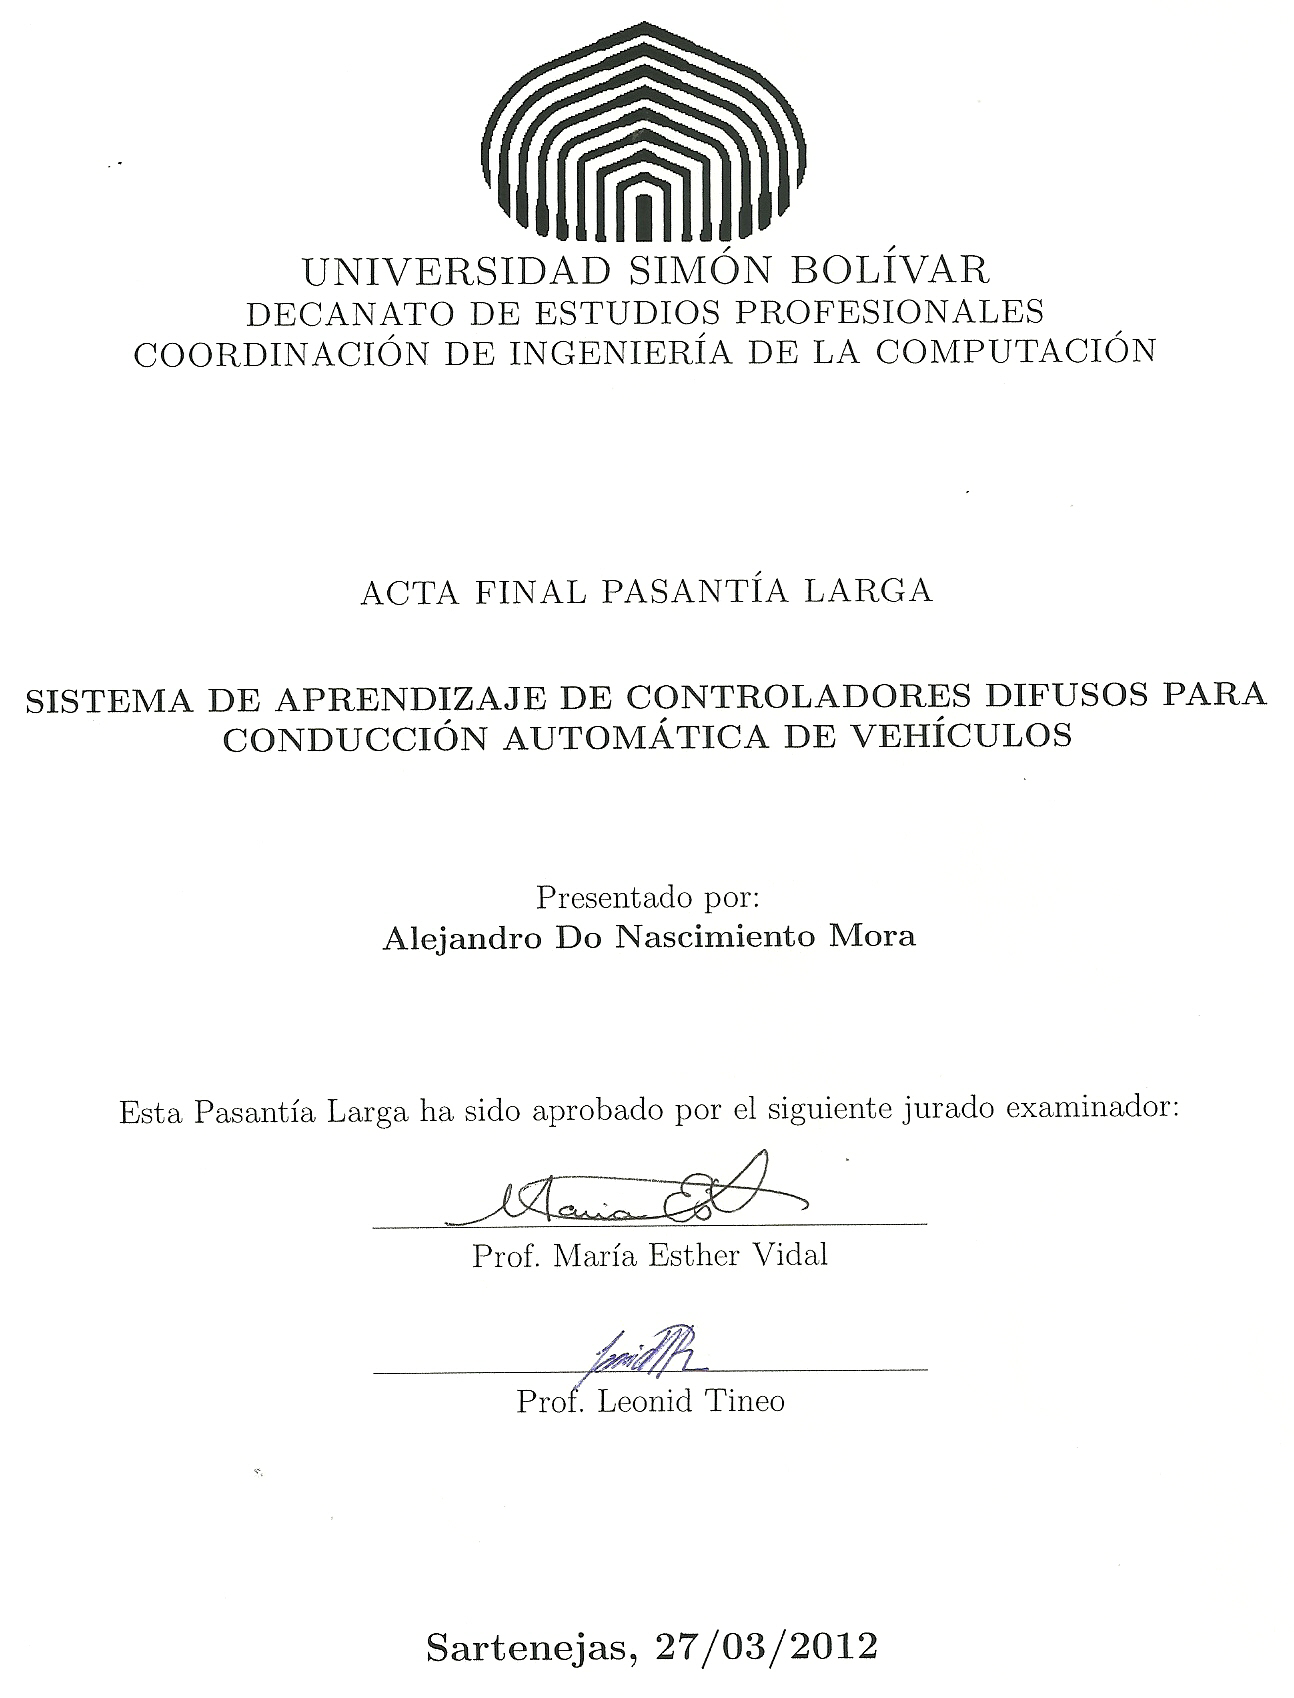
\includegraphics[width=1\textwidth,type=png,ext=.png,read=.png]{acta0001}
\end{figure} 
\end{titlepage}



\setcounter{secnumdepth}{3}
\setcounter{tocdepth}{4}

% Define encabezado numeros romanos y como se separan los captiulos y las
% secciones
\addtolength{\headheight}{3pt}
\pagenumbering{roman}
\pagestyle{fancyplain}

\renewcommand{\chaptermark}[1]{\markboth{\chaptername\ \thechapter:\,\ #1}{}}
\renewcommand{\sectionmark}[1]{\markright{\thesection\,\ #1}}

\onehalfspacing

\lhead{}
\chead{}
\rhead{}
\renewcommand{\headrulewidth}{0.0pt}
\lfoot{}
\cfoot{\fancyplain{}{\thepage}}
\rfoot{}


\begin{onehalfspace}
\setlength{\parskip}{0.5\baselineskip}
% Pagina de resumen
\setcounter{page}{4}
\chapter*{Resumen}



Se presenta un sistema de aprendizaje de controladores difusos, orientado a la conducción autónoma de vehículos, particularmente el control de los pedales, el cual utiliza dos técnicas de aprendizaje, una local y una global, para aprender de los valores de entrada y los resultados generados, con el objetivo de modificar la estructura y parámetros de el controlador difuso.

El aprendizaje local se realiza en tiempo real permitiendo afinar los consecuentes de las reglas correspondientes al controlador difuso. Podemos considerarlo como una respuesta a corto plazo, ya que en cada instante de tiempo, analiza el funcionamiento del controlador, para determinar si es necesario ajustar el modelo que va a ser utilizado en el instante siguiente.

La modificación de la topología y la inserción de nuevas funciones de pertenencia, corresponden al aprendizaje global. Al transcurrir un periodo especifico de tiempo, el sistema analiza el historial de valores de entradas utilizados por el controlador y las funciones de pertenencia a las cuales corresponden, y según el criterio establecido, determina si es necesario, modificar la estructura de las funciones de pertenencia o insertar nuevas funciones de pertenencia.

El sistema fue probado en un entorno virtual utilizando unos 30 vehículos, caracterizados por poseer dinámicas diferentes. Una vez determinado el correcto funcionamiento utilizando vehículos virtuales , se procedió a implementar el sistema en un vehículo real con capacidades de conducción automática, en el cual se utilizaron diferentes configuraciones, con la finalidad de realizar un análisis comparativo y determinar cual genera el mejor desempeño. En ambos casos se obtuvieron muy buenos resultados, incluso en comparación con el modo de conducir de una persona.

\newpage



% Pagina de dedicatoria (opcional)
\setcounter{page}{5}

\vspace*{8cm} 
\pdfbookmark[0]{Dedicatoria}{Dedicatoria} % Sets a PDF bookmark for the dedication
\begin{flushright}
\large \textit{A todas aquellas personas especiales en mi vida\\que me han ayudado y acompañado durante esta travesía.\\En especial a mis padres y a mi hermano, \\ gracias por el apoyo \\ y por darme la oportunidad de vivir esta experiencia.
}
\end{flushright}

\newpage

\end{onehalfspace}
% Crea la tabla de contenidos
\tableofcontents

% Crea la lista de cuadros
\listoftables

% Crea la lista de figuras
\listoffigures

\printglossaries
% Crea la lista de codigos fuentes
%\lstlistoflistings

\clearpage

% Define encabezado en numeros arabicos  
\pagenumbering{arabic}

\fancyhf{} % Redefine el encabezado 
\lhead{}
\chead{}
\rhead{\fancyplain{}{\thepage}}
\renewcommand{\headrulewidth}{0.0pt}
\lfoot{}
\cfoot{}
\rfoot{}

\doublespacing
\renewcommand{\labelitemi}{$\bullet$}
\renewcommand{\labelitemii}{$\circ$}
\newcommand{\rr}{\raggedright}
\newcommand{\tn}{\tabularnewline}

% Incluye los archivos deseados - El contenido de
% su proyecto de grado/pasantia larga.
\setlength{\parskip}{0.5\baselineskip}
\begin{onehalfspace}

% Titulo de la introduccion.
\chapter*{Introducción}
\label{chap:0_Introduccion}
\addcontentsline{toc}{chapter}{Introducci\'on}

% Contenido de la introduccion.
%\section*{Antecedentes:}
\label{sec:Antecedentes}
%Puedes quitar esto(es opcional)

El notable incremento del número de vehículos en las carreteras durante los últimos años ha ocasionado a su vez la proliferación de proyectos de investigación dedicados al desarrollo de \gls{ITS} que permitan optimizar el flujo del tráfico y aumentar la seguridad en las carreteras.

La mayor parte de estas soluciones \gls{ITS} están basadas en el guiado automático de los vehículos.  Durante los últimos 10 años, el grupo AUTOPIA del \gls{CAR} se ha dedicado, en el marco de varios proyectos europeos, a transferir las técnicas desarrolladas para el control de robots móviles a vehículos convencionales, logrando así que la  conducción autónoma de vehículos sea una idea cada vez menos utópica.
	
Con el aumento de prestaciones de los sistemas de localización, sensorización y control, las exigencias son cada vez más importantes. Para conseguir que el control sea lo más seguro y eficaz posible, el conocimiento de la dinámica del vehículo y de su interacción con el entorno es imprescindible.
   
%\section*{Justificación}
\label{sec:justifiacion}


Como resultado del aumento en la motorización, urbanización y la densidad de población, los problemas de congestión de tráfico se han incrementado, reduciendo la eficiencia de la infraestructura de transporte, y ocasionando un aumento en el tiempo de viaje, la contaminación del aire, y el consumo de combustible. Esta serie de problemas han generando mayor interés en la investigación de los \gls{ITS} como posible solución a esta situación y como una manera de hacer más seguro el tránsito por las vías (urbanas e interurbanas).

Uno de los objetivos fundamentales de los \gls{ITS} es aplicar tecnología de la información y la comunicación con el fin de obtener una conducción segura y eficiente. Hoy día, el desarrollo de este tipo de sistemas proporciona una oportunidad de mejorar la seguridad, eficiencia y comodidad en el transporte, ya sea por carretera, aéreo, marítimo o ferroviario\cite{jones_k}

Las acciones involucradas en la conducción de un automóvil pueden ser fácilmente descritas mediante sentencias del tipo: \textit{si el vehículo va a una velocidad menor a la deseada entonces pisar con más fuerza el pedal de aceleración}.  
La lógica difusa trata con la incertidumbre, adjuntando grados de veracidad a la respuesta a una pregunta lógica. En la literatura, desde sus inicios, ha probado ser eficaz y eficiente cuando es aplicada a problemas de la vida real\cite{king}\cite{larsen}\cite{ross}. Comercialmente, la lógica difusa ha sido utilizada con gran éxito en el control de máquinas y productos de consumo. En la aplicación adecuada, los sistemas de lógica difusa son simples de diseñar, y pueden ser comprendidos e implementados por personas no especialistas en el área de teoría de control. 

Los sistemas de control basados en lógica difusa, son utilizados principalmente en situaciones en las cuales un control adecuado es suficiente, ya que no garantizan un resultado óptimo pero si uno aceptable, al igual que resultan candidatos muy fuertes a la hora de enfrentarse con problemas donde la simplicidad y el tiempo de respuesta son factores de gran importancia. Se han aplicado con éxito sistemas de este estilo en las siguientes áreas: aire acondicionado, humidificadores, lavadoras/secadoras, aspiradoras, tostadoras, hornos microondas, refrigeradores, televisión, fotocopiadoras, cámaras de vídeo (Auto-Foco, exposición y Anti-Shake), sistemas Hi-Fi, control climático del vehículo, cajas de cambio automáticas, sistema de tracción en las cuatro ruedas o sistemas de control para espejos y asiento.

%\section*{Planteamiento}
\label{sec:planteamiento}
%Puedes quitar esto(es opcional)

Partimos de la base de que la conducción de un vehículo puede ser fácilmente descrita mediante un conjunto de reglas sencillas, interpretables por una persona sin conocimiento alguno de la dinámica del vehículo, así como sin necesidad de medidas exactas. Este trabajo se enfoca en la creación de un sistema de aprendizaje para controladores basados en lógica difusa, encargados de automatizar el funcionamiento de ciertos controles correspondientes a la conducción. 

El sistema debe poseer la capacidad de adaptarse al funcionamiento de los controladores del vehículo que realizan la automatización, sin la necesidad de tener que especificarle el modelo de funcionamiento de cada uno de ellos, para lo cual a medida que se ejecuta el sistema debe ir aprendiendo sobre la tarea que automatiza.

El aprendizaje se realizará en dos etapas, una llamada aprendizaje local, correspondiente al análisis del comportamiento y los valores obtenidos en la ejecución anterior y otra etapa de aprendizaje global correspondiente a un análisis que abarque lo ocurrido en cada cierto número de iteraciones, o cuando ocurra o se cumpla una situación específica.       


%\section*{Objetivo general}
\label{sec:ObjetivoG}
%Puedes quitar esto(es opcional)

El objetivo global del proyecto es el diseño e implementación de un sistema de aprendizaje que pueda modificar en tiempo real controladores difusos utilizados en conducción autónoma de vehículos. El sistema debe ser capaz de adaptarse a los constantes cambios de dinámicas que podemos encontrar en un vehículo, debidos a, por ejemplo: el número y peso de los ocupantes, la presión y dimensiones de las ruedas, el peso y dimensiones del automóvil, el tipo de tracción, etc., para así tener un sistema de control genérico para vehículos. Los objetivos específicos que se establecieron para poder alcanzar el objetivo general, son los siguientes:

%\section*{Objetivo específico}
\label{sec:ObjetivoE}

\begin{itemize}
\item Familiarización con las técnicas basadas en lógica difusa, ya que se van a utilizar controladores difusos para la automatización de las tareas.
\item Estudio del estado del arte de sistemas difusos adaptativos.
\item Diseño de un método de aprendizaje en tiempo real de los singletons de un controlador difuso.
\item Diseño de un método de aprendizaje de la topología de un sistema difuso.
\item Implementación de dichos métodos de aprendizaje y pruebas tanto en vehículos virtuales como reales.
\item Comparación de bondad frente a un conductor humano.
\end{itemize}

El trabajo está estructurado de la siguiente manera: el primer capítulo describe la institución donde se realizó el trabajo; el capítulo dos corresponde al marco teórico, donde se definen los conceptos de lógica difusa y los controles basados en ella, al igual que se presentan las diversas herramientas utilizadas a lo largo del desarrollo del proyecto; en el tercer capítulo se realiza la descripción y análisis del diseño, el cual esta compuesto por cuatro fases, análisis, diseño, implementación y pruebas; en el capítulo cuatro se explica el desarrollo de la solución; el capítulo cinco presenta las pruebas y resultados obtenidos; en el capítulo seis se explica la adaptación del sistema para el control automático del volante; por último, en el capítulo siete, se encuentran las conclusiones, recomendaciones y trabajos futuros.
%CSIC
\chapter{Entorno institucional} 

En este capítulo se presenta la institución, y el grupo de trabajo perteneciente a dicha institución donde se realizó el proyecto. 

\section{Centro de Automática y Robótica}

	Por un acuerdo entre la \gls{UPM} y el \gls{CSIC}, en 2010 se ha creado el \gls{CAR} como una unidad mixta entre parte del Instituto de Automática Industrial del \gls{CSIC} y la División de Ingeniería de Sistemas y Automática de la \gls{UPM}. El \gls{CAR} se concibe como un centro de investigación en Automática y Robótica cuya estrategia se sustenta en dos grandes pilares: por una parte, la existencia de una actividad investigadora de excelencia que sea referente internacional y, por otra, el impulso de la transferencia de resultados y tecnología a la sociedad y al sector productivo.
	
	La principal seña de identidad del \gls{CAR} será el desarrollo de una investigación de calidad con un planteamiento global y una aproximación multidisciplinar, contribuyendo tanto al avance del conocimiento, como a la resolución de problemas concretos planteados desde distintos ámbitos de la sociedad \cite{car}.
	
\subsection{Objetivos del Centro de Automática y Robótica}

Adquirir conocimientos científicos y tecnológicos al más alto nivel, en el campo de la automatización, cultivando líneas de investigación científica acordes con las prioridades marcadas por el Programa Marco de la Unión Europea y el Plan Nacional de Investigación. Transferir dicha capacidad a la sociedad mediante la implicación del centro en proyectos de innovación. Es decir, participar, realizando tareas de investigación científica y tecnológica, en colaboración con otros organismos y/o empresas, para resolver todos los problemas de desarrollo, industrialización y comercialización que toda auténtica innovación comporta.

\subsection{Grupo AUTOPIA}

El Grupo AUTOPIA se desarrolla en España en el desaparecido Instituto de Automática Industrial, actualmente en el \gls{CAR}, de la \gls{UPM} y el \gls{CSIC}. La línea de investigación principal se orienta hacia la conducción automática de vehículos \cite{utopia}. 

Desde sus inicios en 1998, ha centrado su trabajo en  la aplicación de técnicas de control, desarrolladas primero para robots móviles, en vehículos autónomos reales. Estas técnicas se basan principalemente en lógica difusa, dado que permite el uso de reglas relativamente sencillas para emular el comportamiento humano en conducción de vehículos (\textit{Si el vehículo está desviado hacia la derecha mueve el volante hacia la izquierda}).
El objetivo final es lograr una conducción completamente autónoma, así como mejorar la seguridad en la conducción, principalmente en entornos urbanos y frente a situaciones de alto riesgo. El Grupo ha contado con la financiación proveniente de diversos proyectos de investigación, en la sección \ref{ape:csic} del apéndice, se presentan algunos de ellos.

% Marco Teórico
\chapter{Marco teórico}

En este capítulo se presentan los conceptos y recursos utilizados en el proyecto. En las \textbf{secciones \ref{sec:ld}} y \textbf{\ref{sec:contrdi}}, se habla sobre la teoría de lógica difusa y controladores difusos respectivamente; \textbf{La sección \ref{sec:sde}} trata el concepto de sistemas difusos evolutivos; la \textbf{sección \ref{sec:orbex}} presenta la librería de lógica difusa que se utilizó para desarrollar el sistema de aprendizaje; la pista y el vehículo utilizado para las pruebas se introducen en las \textbf{secciones \ref{sec:zoco}} y \textbf{\ref{sec:carros}}; por último la sección \textbf{\ref{sec:carros}} trata sobre el simulador utilizado durante la realización del proyecto.   

\section{Lógica difusa} 
\label{sec:ld}
En la década de los 60, Lotfi Zadeh, un profesor matemático iraní residente en los Estados Unidos, describe los fundamentos matemáticos asociados a la teoría de conjuntos difusos y por extensión a la lógica difusa (\textit{Fuzzy logic}) \cite{zadeh1965fuzzy}.

La lógica difusa es una lógica multievaluada, que en vez de trabajar con el modelo clásico de inclusión y exclusión, remplaza los dos valores de veracidad verdadero y falso ($\{0,1\}$), por un continuo de valores, generalmente representados por el intervalo $[0,1]$. 

Una de las principales aplicaciones de la lógica difusa es el modelado del razonamiento humano en situaciones donde se posee información vaga, incompleta y/o (parcialmente) contradictoria; normalmente en la forma de sistemas basados en reglas. 

Los conjuntos difusos, que están basados en esta lógica, pueden ser utilizados para modelar la vaguedad lingüística escondida en atributos como \textit{grande} y \textit{pequeño} y, en particular, la transición gradual entre ellos. Éstos se presentan a continuación.


\subsection{Conjuntos difusos}
\label{sec:cd}

La teoría de conjuntos difusos expresa imprecisiones de manera cuantitativa, por medio de introducir una función que refleja el grado de pertenencia de un valor hacia un atributo, adoptando valores que pertenecen al intervalo [0,1].

Un conjunto difuso es un par $(A,m)$ donde $A$ es un conjunto y $m : A \longrightarrow [0,1]$.
Para cada $x \in A, m(x)$ es llamado el grado de pertenencia de $x$ en $(A,m)$.

\begin{figure}[htb]
\centering
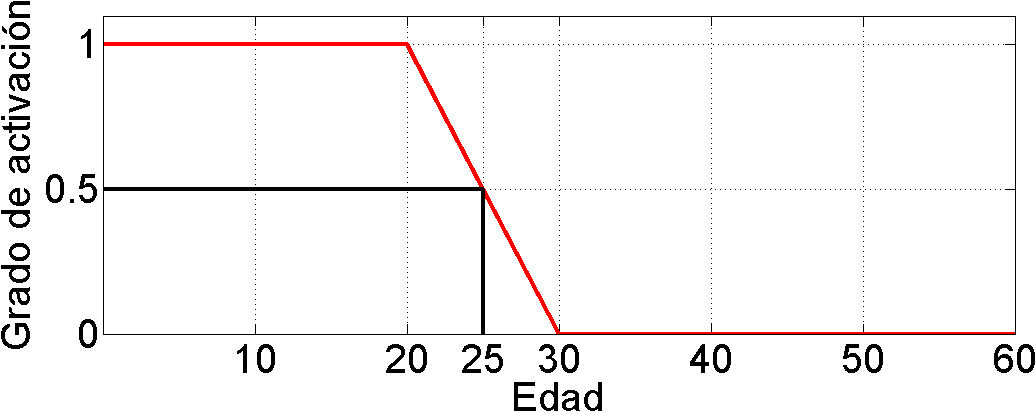
\includegraphics[width=0.55\textwidth,type=png,ext=.png,read=.png]{figures/conjunto_difuso}
\caption{Conjunto difuso que representa a grupo de personas jóvenes.}
\label{fig:conjunto}
\end{figure} 

En la figura \ref{fig:conjunto} se observa un ejemplo del conjunto difuso que representaría a las personas \textit{jóvenes}. De 0 a 20 años diríamos que las personas pertenecen completamente al grupo de gente joven, pero a medida que va aumentando la edad, va reduciendo su grado de pertenencia al conjunto de los jóvenes. De esta forma, con unos 25 años todavía se seria joven al 50 \%, y a partir de 30 años dejaría de pertenecer al grupo. 

En los sistemas de control basados en lógica difusa, la forma más común utilizada en las funciones de pertenencia es el triángulo, aunque otras como los trapecios y la curva de bell también son muy utilizados. De tres a siete curvas es generalmente apropiado para cubrir los rangos sobre los  que se están trabajando, así como no supone un esfuerzo notable para el diseñador, el trabajar con ellas. 

\begin{figure}[htb]
\centering
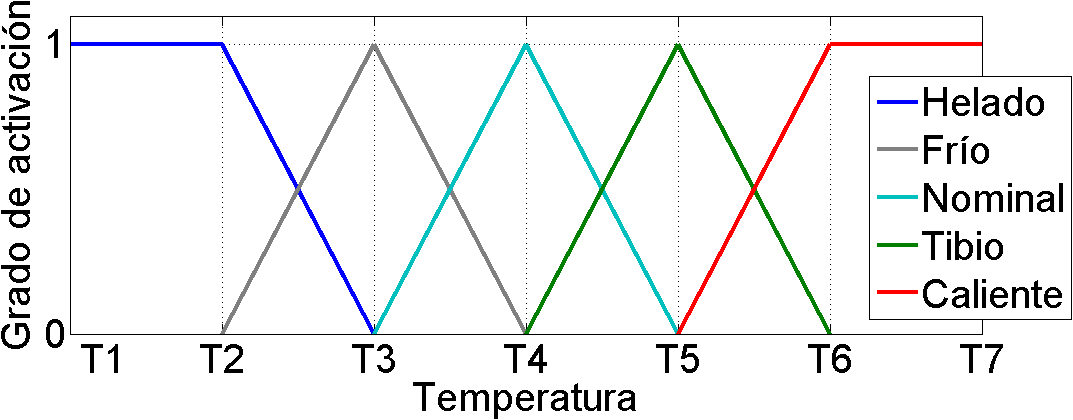
\includegraphics[width=0.55\textwidth,type=png,ext=.png,read=.png]{figures/fpertenencia}
\caption{Sistema difuso correspondiente a la temperatura, con cinco funciones de pertenencia. Cada etiqueta o función de pertenencia corresponde a un nivel de temperatura.}
\label{fig:fpertenencia}
\end{figure} 

%Puedes quitar esto(es opcional)

\section{Controladores difusos} 
\label{sec:contrdi}


Los controladores difusos aplican la teoría de conjuntos difusos para definir y resolver problemas de control. Contienen una colección de funciones de pertenencia y reglas que son utilizadas para razonar sobre datos. Trabajan de una manera diferente a los controladores convencionales, ya que utilizan el conocimiento experto en lugar de ecuaciones diferenciales para describir un sistema y su comportamiento. 

Dicho conocimiento se representa de manera natural,  por medio del uso de variables lingüísticas que representan conjuntos difusos; describiendo así, el conocimiento de una manera similar a como lo haría un experto. 

Se define la \textbf{topología del controlador} como la cantidad, forma que poseen y la manera en que se encuentran distribuidas, las etiquetas o funciones de pertenencias, que han sido asignadas a lo largo de los rangos establecidos para cada una de las variable de entrada.

Su funcionamiento se descompone en una etapa de entrada, una de procesamiento y una de salida. En la \textbf{etapa de entrada}, se asignan los grados de pertenencia a los conjuntos difusos correspondientes, en función de los valores de entrada. La \textbf{etapa de procesamiento} evalúa las reglas involucradas y genera un grado de veracidad a las mismas, para luego combinar el resultado de las reglas. Finalmente, la \textbf{etapa de salida} convierte el resultado obtenido en un valor salida específico. 

Los sistemas difusos están formados principalmente por cuatro componentes, y siguen un esquema como el que se presenta en la figura \ref{fig:controlador}. 
Cada una de las etapas que definen el funcionamiento de un controlador difuso se detallan en las siguientes subsecciones.


\begin{figure}[htb]
\centering
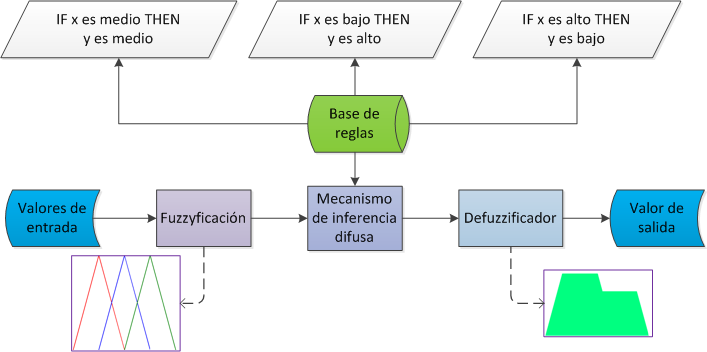
\includegraphics[width=0.7\textwidth,type=png,ext=.png,read=.png]{figures/sistemad}
\caption{Esquema de procesamiento general de un sistema difuso.}
\label{fig:controlador}
\end{figure} 



\subsection{Fuzzificador}


La entrada de un sistema basado en lógica difusa es, por lo general, un valor numérico. Para que este valor pueda ser procesado por el sistema difuso se hace necesario convertirlo a un \textit{lenguaje}  para que el mecanismo de inferencia pueda procesarlo. 

La función del \textit{fuzzificador} es la de realizar tal conversión. Éste toma los valores numéricos provenientes del exterior y los convierte en valores \textit{difusos} para que puedan ser procesados por el mecanismo de inferencia. Estos valores difusos están representados por los grados de pertenencia de los valores de entrada a los diferentes conjuntos difusos en los que se ha dividido el universo de discurso de cada una de las variables de entrada.


\subsection{Mecanismo de inferencia difusa}


Teniendo los diferentes niveles de pertenencia arrojados por el fuzzificador, los mismos deben ser procesados para general una salida difusa. La tarea del sistema de inferencia es tomar los niveles de pertenencia y apoyado en la base de reglas generar la salida del sistema difuso.


\subsection{Reglas de control difuso}


La base de reglas es la manera que tiene el sistema difuso de almacenar el conocimiento lingüístico que le permite resolver el problema para el cual ha sido diseñado.

Describe la metodología o el conjunto de reglas que aplicaría un ser humano encargado de controlar el proceso, con toda la imprecisión que poseen los lenguajes naturales y, sólo a partir de estas reglas, generar las acciones de control. La base de reglas se representa mediante un conjunto de reglas del tipo:

\begin{center}
\begin{alltt}
IF \textit{x1} es pequeño AND \textit{x2} es grande THEN \textit{y} es medio 
IF \textit{x1} es pequeño AND \textit{x2} es medio THEN \textit{y} es grande 
\end{alltt}
\end{center} 

Estas expresiones de la forma \textit{IF...THEN...} son las reglas de control difuso. Las variables de condición $x1, x2, ...,$ representan las variables de entrada del sistema, y se ubican en el antecedente; la variable $y$ es la salida del mismo, y pertenece al consecuente, las palabras \textit{pequeño}, \textit{grande} y \textit{medio} son los conjuntos difusos en los que se codifica la variable de entrada.

Los controladores difusos contienen grupos de reglas y actúan de la forma siguiente: Cuando se les proporciona el valor actual de las variables de entrada se obtiene el valor de verdad de las reglas, calculado mediante un método de \textit{inferencia difusa}. 

Teniendo en cuenta que los sistemas de control deben actuar en tiempo real, los métodos de inferencia que se usan suelen ser sencillos y rápidos.  


\subsection{Defuzzificador}


La salida que genera el mecanismo de inferencia es una salida difusa, por lo que no puede ser interpretada por un elemento externo (por ejemplo un controlador) que solo manipule información numérica. 

Para lograr que la salida del sistema difuso pueda ser interpretada por elementos que sólo procesen información numérica, hay que convertir la salida difusa en un valor numérico; este proceso lo realiza el \textit{defuzzificador}. Para generar la salida numérica a partir de este conjunto existen varias opciones como el Centro de Gravedad, los Centros Promediados entre otros.

\section{Sistemas difusos evolutivos} 
\label{sec:sde}

Pueden definirse como sistemas de auto-desarrollo y auto-aprendizaje basados en lógica difusa, en los cuales, tanto sus parámetros como su estructura, alcanzan un estado de auto-adaptación \textit{on-line}.

Generalmente son asociados con flujo de datos y modos de operación \textit{on-line} (a menudo en tiempo real). Pueden ser vistos como sistemas difusos adaptativos. La diferencia es que los sistemas difusos evolutivos asumen la adaptación en línea de la estructura del sistema, ademas de la adaptación de parámetros, que es usualmente asociada con el termino adaptativo. También permiten la adaptación del mecanismo de aprendizaje. De esta manera, evolutivo asume un nivel superior a adaptativo. 

Uno de los problemas de los controladores (particularmente los controladores difusos), es el diseño y la configuración precisa. Debido al cambio constante en el ambiente de operación de las plantas industriales y los controladores, el diseño y configuración \textit{off-line} no proporciona la flexibilidad que es requerida. La teoría de control adaptativo nos provee con una manera para resolver esta situación, basada en la adaptación constante de los parámetros del (usualmente linear) controlador. Los problemas reales, generalmente no son lineales, ni estacionario, por lo tanto, la teoría de control adaptativa, tiene sus obvias limitaciones.
 
Los controladores difusos evolutivos basados en reglas \cite{angelov04}\cite{Angelov02}, combinan la flexibilidad y naturaleza no linear de los sistemas difusos, con las ventajas de los esquemas adaptativos bien establecidos.  

\section{ORBEX} 
\label{sec:orbex}

Los controladores utilizados por el programa de control utilizado en el grupo AUTOPIA están definidos utilizando la librería de modelado difuso \gls{ORBEX} \cite{Garcia1998}, la cual sigue un esquema como el que se presenta en la sección \ref{sec:contrdi}. El entorno ha sido usado por el grupo AUTOPIA para el modelado y ejecución en tiempo real de los controladores difusos que controlan los vehículos. 

Con los controladores definidos por \gls{ORBEX}, se pueden describir diferentes formas de conducción con el fin de emular comportamientos de diferentes tipos de conductores y adaptar la conducción a la situación actual del tráfico. Dichas estrategias pueden ser definidas e implementadas mediante reglas difusas del tipo \textit{IF...THEN...}

\gls{ORBEX} trabaja con controladores difusos que utilizan funciones de pertenencia trapezoidales para la codificación de las variables de entrada, y \textit{\gls{singletons}} para la codificación de variables de salida. Esto permite tomar decisiones de control en un período de tiempo muy corto, con muy buena precisión y garantizando la estabilidad del sistema. 

Los \textbf{singletons} son conjuntos que poseen un único elemento, se utilizan como el consecuente de las reglas difusas que definen al controlador. Representan el valor que va ha ser aplicado, una vez que se active, o se cumpla, la regla correspondiente.

Para el diseño de un controlador con \gls{ORBEX} es necesario especificar 3 secciones fundamentales:
\begin{itemize}
    
    \item Las variables de entrada al sistema con sus respectivas particiones difusas o etiquetas lingüísticas.
    
    \item Las variables de salida del sistema con sus respectivas particiones (\gls{singletons}). 
    
    \item Un conjunto de reglas de inferencia que operan sobre las variables de entrada y de salida de tal forma que a las variables de salida les sea asignado un valor.
\end{itemize}

El número de reglas de los controladores que se utilizaron en el proyecto, es igual al producto entre el número de etiquetas o funciones de pertenencia que hallan sido asignadas a cada variable de entrada, por lo la base de datos de las reglas presenta un crecimiento exponencial al insertarse una nueva etiqueta. Una regla de un controlador con dos variables de entradas es de la siguiente forma:

\begin{center}
{\tt SI Entrada0 ET01 Y Entrada1 ET12 ENTONCES Pedal Ped5} \hspace{4 cm}(2.1)
\end{center} 

Donde \verb,Entrada0, y \verb,Entrada1, son los valores de entrada. \verb,ET01, es la etiqueta o función de pertenencia número uno de la variable de entrada cero, y \verb,ET12, es la etiqueta dos de la variable de entrada uno, ambas etiquetas poseen forma trapezoidal, se definen especificando el valor de las coordenada en el eje $x$ de cada vértice del trapecio, las coordenada en $y$ son asignadas automáticamente por \gls{ORBEX}, siendo cero para el primer y último valor, y  uno para el segundo y el tercero. \verb,Ped5, es el singleton que representa el consecuente de la regla, es el valor que se debe aplicar cuando e activa o se cumple con un cierto grado esta regla, un posible valor para \verb,Ped5, puede ser -0.10552.  

Para una explicación más detallada sobre el diseño de controladores con \gls{ORBEX}, referirse a la sección \ref{ape:diseno} del apéndice.

La gramática de \gls{ORBEX} (ver apéndice \ref{ape:gramatica}), nos permite el uso de modificadores lingüísticos, éstos se presentan en la tabla \ref{modificadores}, cada uno con su función de cómputo asociada, donde $\mu$ representa el grado de pertenencia del valor de la variable de entrada a un determinado subconjunto difuso.

\begin{table}[htb]
  \centering
  \begin{tabular}{|c|c|}
    \hline
    % after \\: \hline or \cline{col1-col2} \cline{col3-col4} ...
    \rowcolor[gray]{0.9} \textbf{Modificador} & \textbf{Cálculo} \\
    \hline
    \hline
    \textit{POCO} & $\sqrt{\mu}$ \\ \hline
    \textit{MUY} & $\mu^{2}$ \\ \hline
    \textit{EXTRA} & $\mu^{3}$ \\ \hline
    \textit{MAYORQUE(a)} & $\mu_{>a}$ = 1 - $\mu_{a}$\\ \hline
    \textit{MENORQUE(a)} & $\mu_{<a}$ = 1 - $\mu_{a}$ \\ \hline
    \textit{ENTRE(a,b)} & MAYORQUE(a) x MENORQUE(b) \\ \hline
    \textit{NO} & 1-$\mu$ \\
    \hline
  \end{tabular}
  \caption{Modificadores Lingüísticos soportados por ORBEX}
  \label{modificadores}
\end{table}

En la sección \ref{ape:orbex} del apéndice se presenta un ejemplo de un controlador definido en \gls{ORBEX}.

Otro aspecto a tener en cuenta sobre el proceso de inferencia usado por \gls{ORBEX}. Una vez establecido el valor de las variables de entrada, el sistema realiza el proceso de \textit{fuzzificación}, que asigna un valor de pertenencia a cada subconjunto o partición difusa de la variable según el valor \textit{crisp} asignado a la variable. Una vez hecho esto, se procede a la inferencia, que sigue el siguiente procedimiento estándar para cada una de las reglas:

\begin{enumerate}
    \item Se calcula primero el grado de cumplimiento de la primera condición
    \item Se asigna este cumplimiento a una variable temporal \{\textit{W}\}
    \item Se calcula el grado de cumplimiento de la segunda condición
    \item Se calcula el conectivo lógico \{\textit{Y/O}\} mediante las t-normas y s-normas mínimo y máximo
    \item Se guarda el resultado en la variable temporal \{\textit{W}\}
    \item Se calcula el grado de cumplimiento de la tercera condición
    \item Se calcula el conectivo lógico \{\textit{Y/O}\} mediante las t-normas y s-normas mínimo y máximo
    \item Así, en general para \textit{N} condiciones y conectivos lógicos.
\end{enumerate}

El valor final de la variable temporal \{\textit{W}\} representará el grado de satisfacción del antecedente de la regla y que este valor será el peso que se asigne al consecuente de la regla. Una vez realizado el proceso de inferencia, se pasa al proceso de \textit{defuzzificación}, que consiste en la suma ponderada de los singletons de la variable de salida, según la siguiente fórmula $\frac{\sum P_{i}w_{i}}{\sum w_{i}}$,
donde $w_{i}$ es el peso correspondiente a la partición difusa singleton $P_{i}$.

%\begin{equation}
%    \frac{\sum P_{i}w_{i}}{\sum w_{i}}
%\end{equation}
%\noindent donde $w_{i}$ es el peso correspondiente a la partición difusa singleton $P_{i}$.

\section{ZOCO}
\label{sec:zoco}

\gls{ZOCO} es una pista de pruebas de vehículos automáticos que está dedicada exclusivamente a tareas de
investigación, es decir, en ella no hay ningún otro tráfico de vehículos, lo que se ha hecho por razones de seguridad. Tiene una
forma reticulada, como las manzanas o cuadras de una ciudad, con algunas irregularidades, con calles de seis metros de ancho,
permite la circulación en ambos sentidos. En la figura \ref{fig:zoco} se puede ver una vista aérea de \gls{ZOCO}\footnote{Fuente: \url{http://maps.google.es}}.

Las calles horizontales tienen nombres de personajes dedicados a la automatización, mientras que las verticales están dedicadas a antiguos científicos y personajes que diseñaron y crearon instrumentos de navegación (ver anexo \ref{ape:zoco}).

\begin{figure}[h]
  \centering
  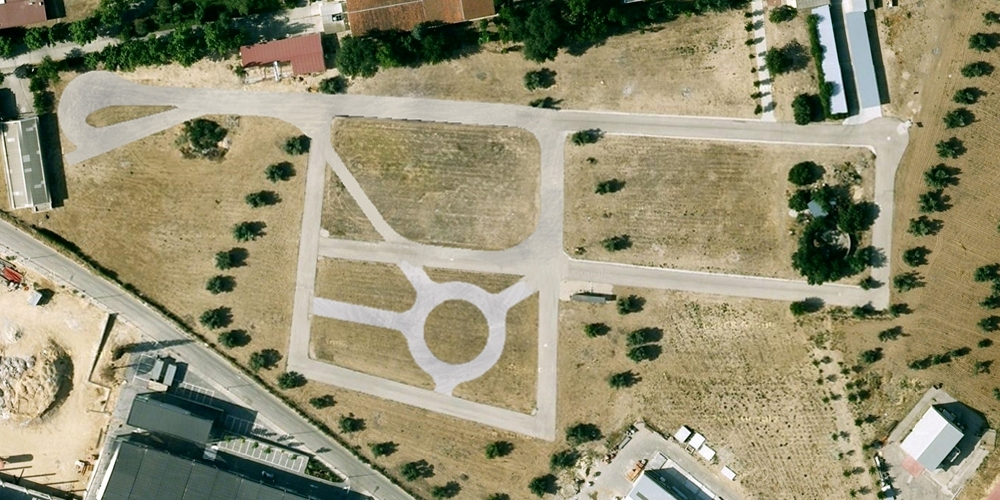
\includegraphics[width=0.5\textwidth]{figures/zoco.png}
  \label{zoco}
  \caption{Vista aérea de ZOCO}
  \label{fig:zoco}
\end{figure}

Estos nombres de calles nos permiten especificar los recorridos que han de hacer los coches de una manera simbólica, estos recorridos son transformados por un intérprete en un conjunto de maniobras elementales, evidentemente, el intérprete ha de poseer un mapa de \gls{ZOCO}.

\gls{ZOCO} también dispone de una estación base de posicionamiento global diferencial basado en información geográfica vía satélite, \gls{DGPS}, que puede ser utilizado por sistemas móviles embarcados en los coches para obtener su posición con una precisión inferior al centímetro \cite{Milanes2008a} \cite{Milanes2008b}. 

Existe una estación central de coordinación sobre la que se prueban las estrategias, normalmente basadas en lógica difusa, que luego son transferidas a los coches \cite{GodoyBilbao2010}.

\section{Vehículos automatizados}
\label{sec:carros}

La flota de vehículos del grupo AUTOPIA esta formada por 5 automóviles (ver sección \ref{ape:carros} en el anexo), de los cuales utilizaremos un \textbf{Citroën C3 Pluriel}, llamado \textbf{Platero}, para realizar las pruebas experimentales del sistema desarrollado en este trabajo.

\begin{figure}[ht]
\begin{minipage}[b]{0.5\linewidth}
\centering
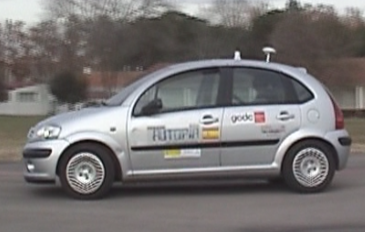
\includegraphics[width=0.9\linewidth]{figures/platero.png}
\caption{Platero}
\label{fig:platero}
\end{minipage}
\begin{minipage}[b]{0.5\linewidth}
\centering
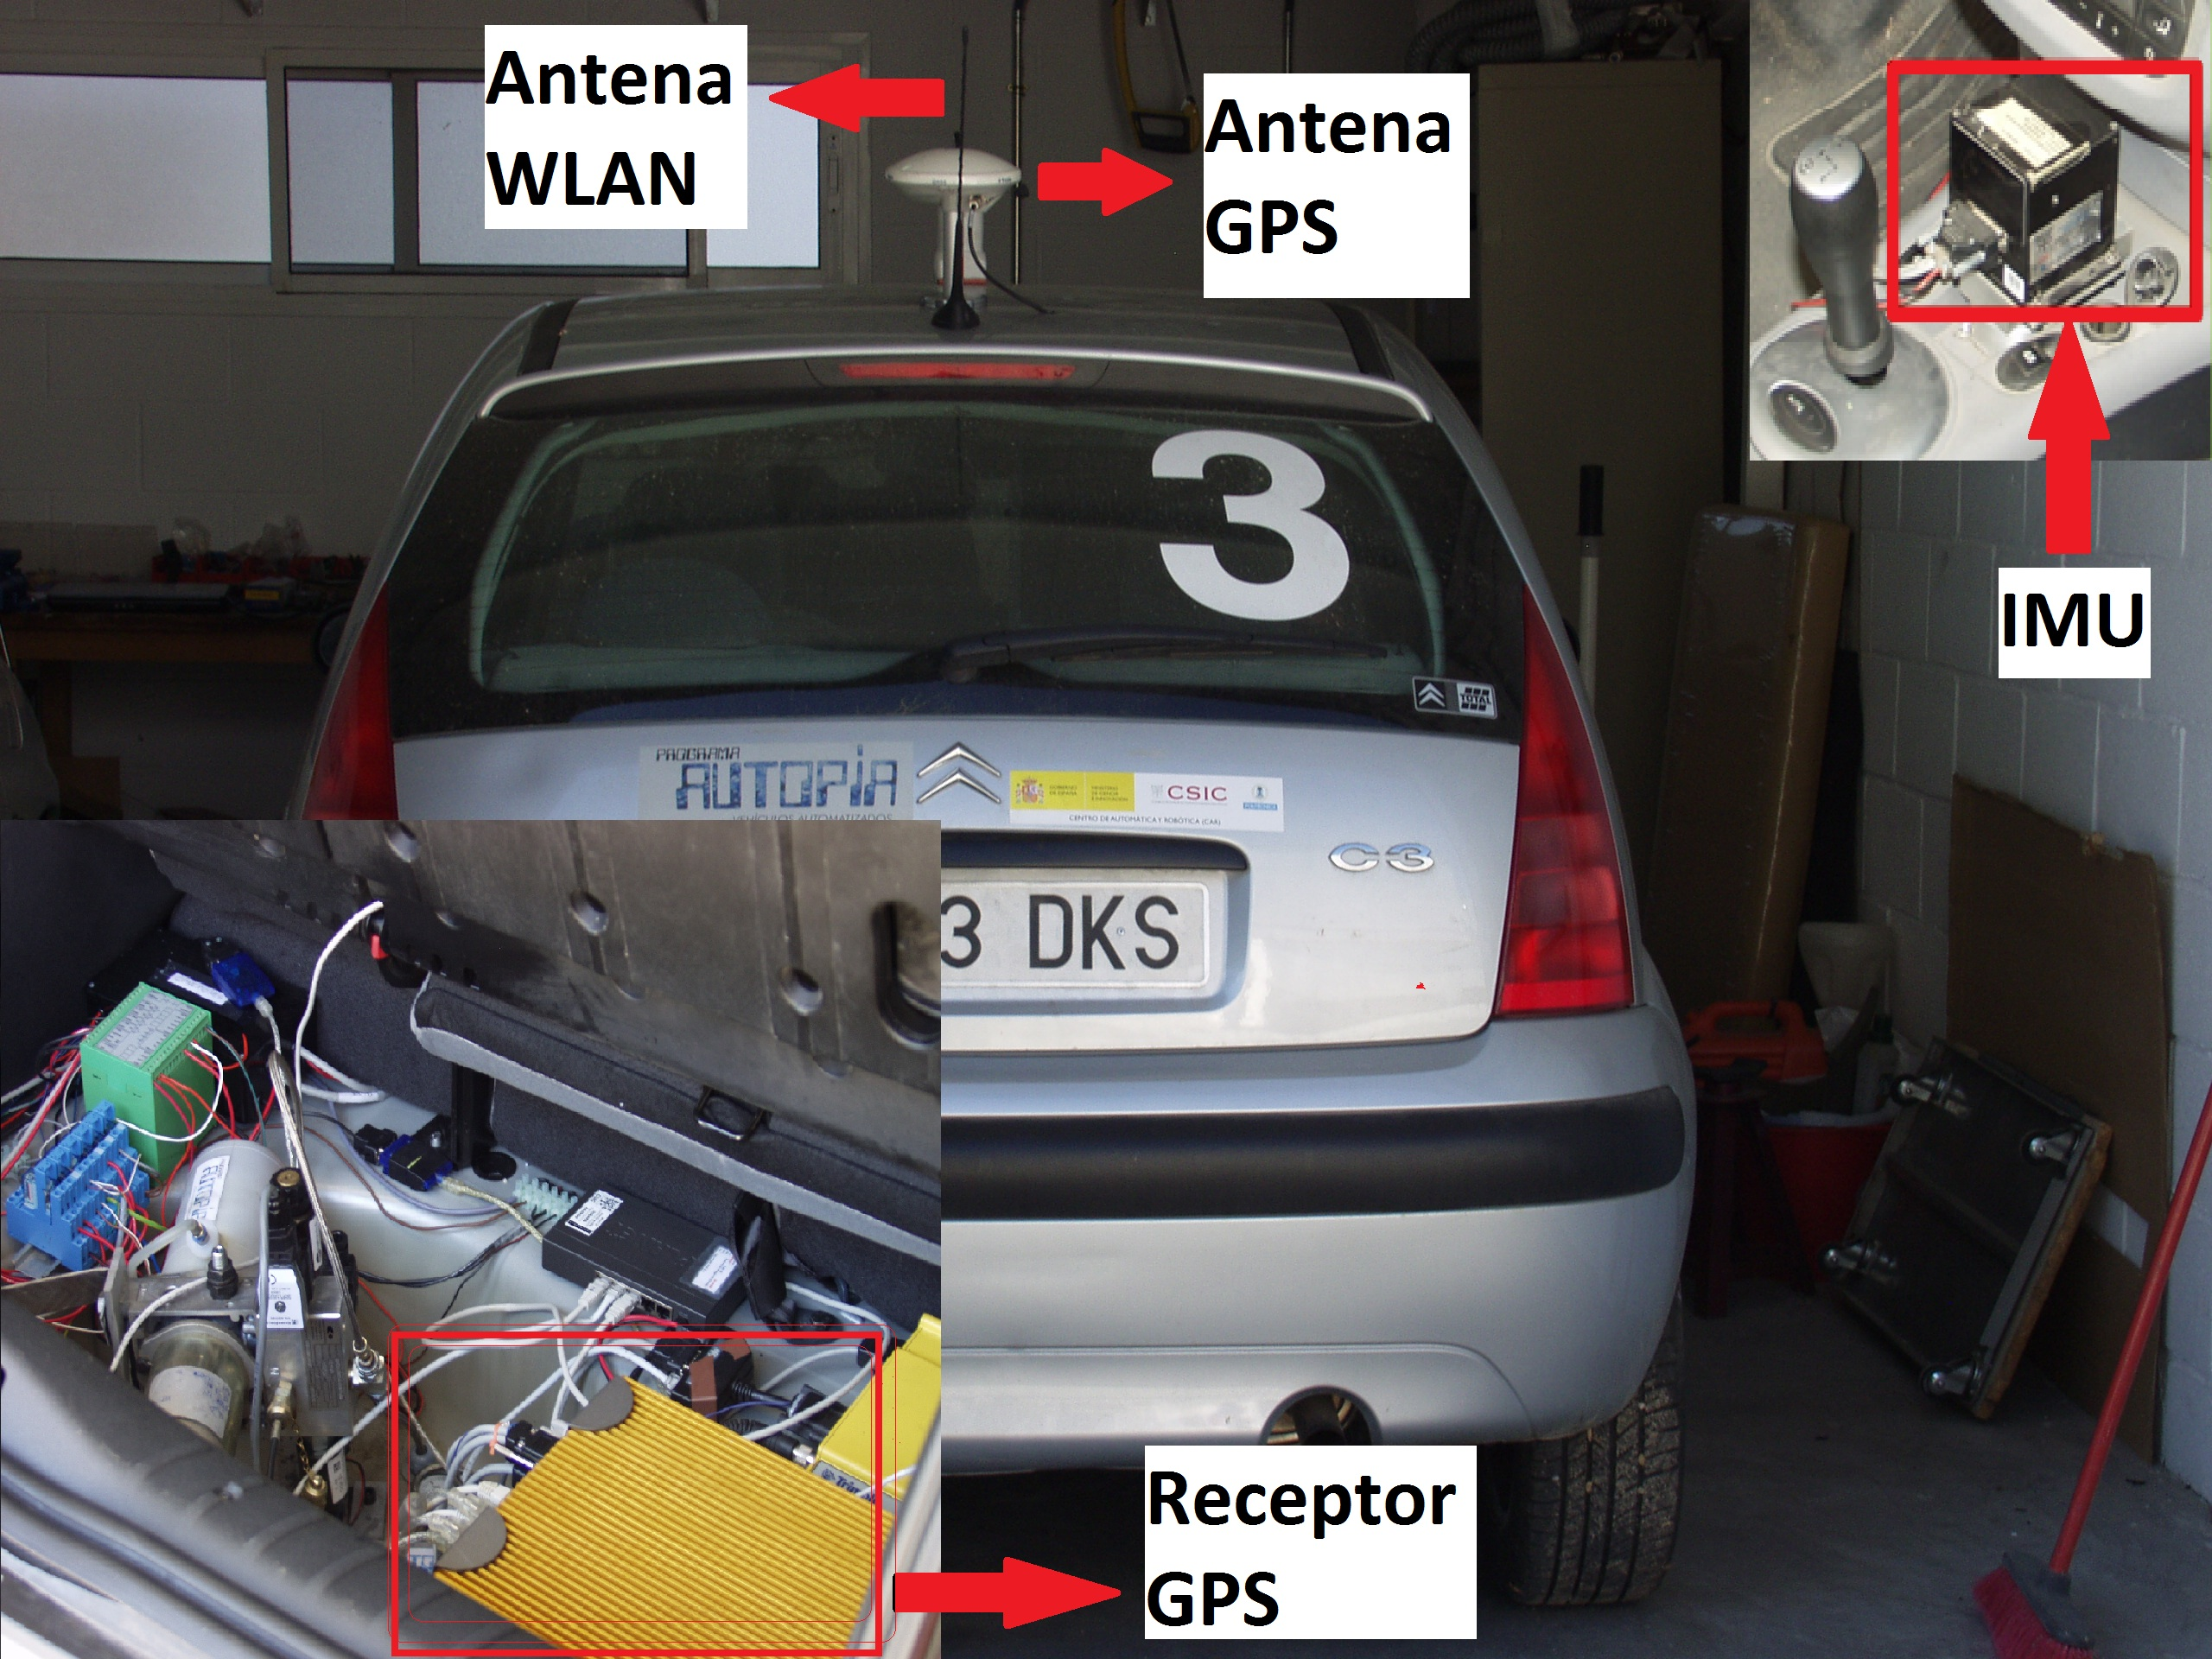
\includegraphics[width=0.9\linewidth]{figures/maletero.jpg}
\caption{Instrumentación de Platero}
\label{fig:maleta}
\end{minipage}
\end{figure} 
\interfootnotelinepenalty=10000
Platero está instrumentado para actuar sobre los pedales acelerador/freno y sobre volante, ambos sistemas pueden funcionar conjunta o independientemente. Posee un sistema de navegación, formado principalmente por un \gls{GPS}, un sistema para comunicarse con la estación base vía \gls{WLAN}, y un bus \gls{CAN}\footnote{Red interna del vehículo donde circulan mensajes y órdenes, tales como subir bajar ventanas, cambiar a segunda velocidad, encender luces intermitentes, ...}, del cual se obtienen variables, tales como la velocidad, aceleración,.. o bien se pueden recibir órdenes de control. En esta sección se enfoca en los controles de aceleración y freno, para un descripción más detallada de los otros sistemas de Platero, referirse a la sección \ref{ape:platero} del apéndice.

En lo que se refiere a la actuación necesaria para llevar a cabo un control de velocidad, se debe tener en cuenta únicamente el manejo de los pedales de acelerador y freno, dado que el vehículo utilizado (\textit{Platero}) dispone de su propio sistema de cambio de velocidades de la transmisión automático implementado por Citroën.

Para lograr el control sobre el \textbf{acelerador}, se cortaron las dos señales de tensión que genera el acelerador y se conmutaron por otras generadas por el ordenador embarcado del vehículo. Para el control del \textbf{freno}, se intervino la caja del \gls{ABS} con un sistema de actuación que consta de una válvula con una salida, conectada directamente al \gls{ABS} para respetar el circuito original. El sistema consta de dos entradas: la primera conectada al circuito inicial de freno, que permite su accionamiento convencional, y la segundo conectada a un sistema electro-hidráulico diseñado para el accionamiento automático del freno desde el ordenador embarcado.

Por otra parte, el funcionamiento de los sistemas de actuación no impide que un usuario pueda actuar sobre los pedales en caso de emergencia, o desactivarlos para realizar una conducción manual cuando lo desee. Con el sistema automático activado, el ordenador generará ordenes de control en el intervalo [0,1] que se traducirán en porcentaje de presión a aplicar sobre el correspondiente pedal.

\section{TORCS}
\label{sec:torcs}

\gls{TORCS} es un simulador de carros multiplataforma y altamente portable. Es utilizado como un juego ordinario de carreras, como un juego de carreras de inteligencia artificial y como una plataforma de investigación. Es compatible con \gls{Linux} (\gls{x86}, \gls{AMD64} y \gls{PPC}), \gls{FreeBSD}, \gls{MacOSX} y \gls{Windows}. El código fuente de TORCS esta licenciado bajo \gls{GPL}.

\begin{figure}[ht]
\begin{minipage}[b]{0.5\linewidth}
\centering
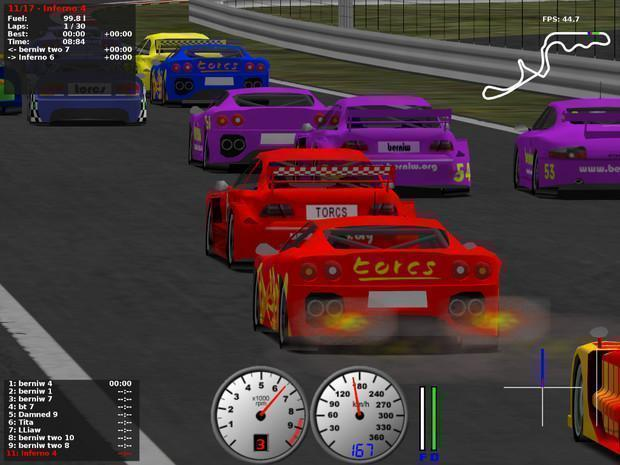
\includegraphics[width=0.7\linewidth]{figures/torcs_screenshot3.jpg}
\end{minipage}
\begin{minipage}[b]{0.5\linewidth}
\centering
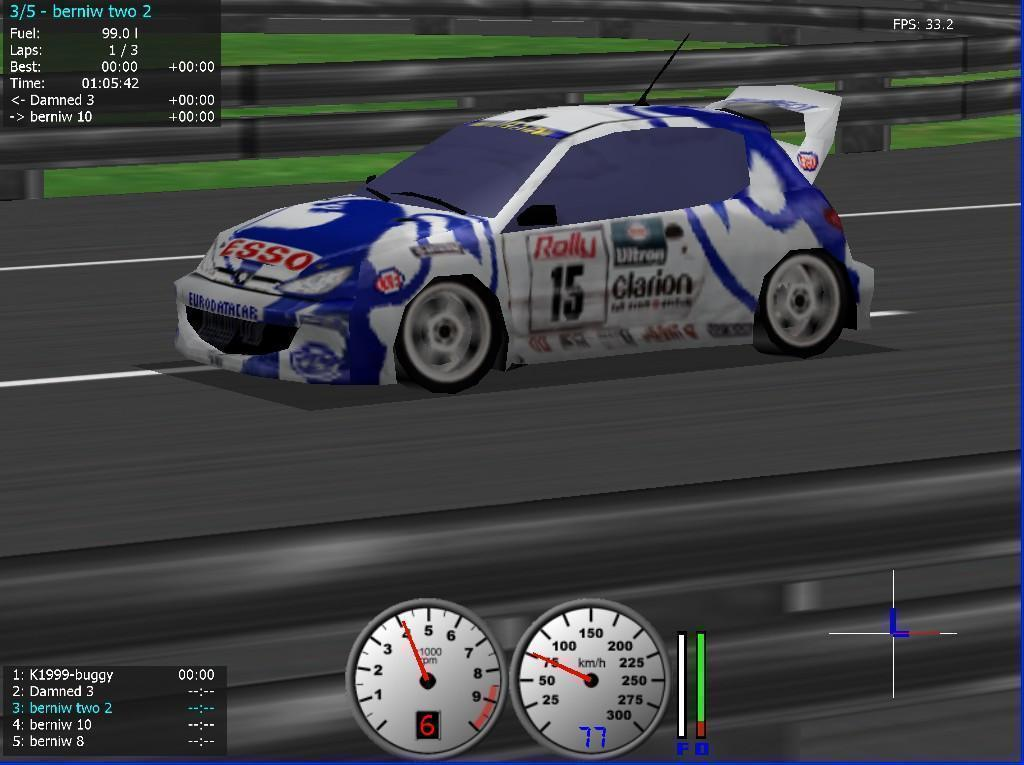
\includegraphics[width=0.7\linewidth]{figures/torcs3.jpg}
\end{minipage}
\caption{Captura de pantalla de \gls{TORCS}.}
\end{figure} 

A nivel de simulación posee un modelo de daños simple, colisiones, propiedades de frenado y ruedas (rigidez, humedad, brincos,…), aerodinámica (efecto del suelo, spoilers,…) y muchos más.

Lo elegimos como plataforma para realizar las simulaciones por varias razones: todo su código es \gls{Open Source}; la implementación del juego esta diseñada para facilitar al programador el desarrollo de robots inteligentes de una manera fácil y sencilla; un entorno gráfico agradable, sobre el cual se puede ver el comportamiento del vehículo; un modo texto, el cual reduce el tiempo de ejecución de las simulaciones considerablemente; un entorno virtual muy fiel a la realidad cumpliendo con la mayoría de las leyes físicas fundamentales como gravedad, coeficiente de fricción, aerodinámica, daños en el carro, consumo de combustible, balance de masa, etc.; más de 30 pistas distintas, de características muy dispares, anchura de pista, longitud, tipo de superficie, etc.; posibilidad de elegir entre casi 50 vehículos distintos.         

\chapter{Descripción y análisis del diseño}
\label{chap:3_Descripcion}

Este capítulo ofrece una visión acerca de los lineamientos seguidos para el diseño del desarrollo del proyecto, especificando la metodología utilizada y las cuatro fases que esta involucró. Para el desarrollo del sistema, se definieron cuatro etapas básicas, descritas a continuación.


\section{Fase de análisis}
\label{subsec:analisis}


Consistió en definir el objetivo general del proyecto, objetivos específicos, y cada una de las funcionalidades que se querían implementar. Se consultaron trabajos correspondientes al área de estudio a la que pertenece nuestro trabajo \cite{servo} \cite{online} \cite{two} \cite{adaptive} , para determinar los métodos de aprendizaje que se han implementado y analizar los resultados de tales sistemas.

Se hizo un análisis de la librería de lógica difusa \gls{ORBEX} (sección \ref{sec:orbex}), los tipos de funciones de pertenencias que soporta, la manera en que maneja y procesa los datos. Al igual que un estudio sobre la herramienta de simulación \gls{TORCS}, y los vehículos del grupo AUTOPIA que se van utilizar para las pruebas, para determinar si los resultados obtenidos con las simulaciones son representativos de una prueba realizada con los automóviles. A partir de este estudio, se determinaron los sistemas de control a desarrollar, eligiéndose un sistema para controlar la velocidad por medio de los pedales, y en caso de contar con tiempo suficiente, desarrollar uno para el control de la dirección del carro por medio del volante. 

En esta fase se determinaron las métricas a utilizar como variables de entradas para el controlador del pedal, seleccionando el error y la derivada del error como las dos principales, y en caso de realizar pruebas con una tercera variable de entrada, se eligió el perfil de velocidad del vehículo (sección \ref{sec:acondicionamiento}). 

\section{Dise\~no}
\label{subsec:diseno}


Se buscó un diseño de la forma más general posible, con el fin de utilizarlo para el control de cualquier tarea, teniendo en cuenta una variable de confort, para evitar cambios muy bruscos en los valores de salida.

Para lograr una integración más cómoda y práctica con el programa que utilizan los vehículos del grupo AUTOPIA, se implementó el cálculo de los valores de entrada directamente dentro del sistema, para evitar tener que modificar el programa del carro con la inclusión de funciones nuevas.

Para poder realizar un análisis del funcionamiento del sistema de control, se optó por la creación de un archivo, que posee todo los datos correspondientes a la ejecución del sistema. 


\section{Implementación}
\label{subsec:implementacion}


La fase de implementación se realizó principalmente en tres partes (ver capítulo \ref{chap:4_Desarrollo}), se comenzó por el aprendizaje local que consiste en la modificación del consecuente de las reglas, luego el aprendizaje global que se encarga de la modificación de la topología del controlador difuso, y se finalizó con una etapa de ajuste, en la cual se realizaron modificaciones principalmente al aprendizaje local.

El proceso estuvo caracterizado por ser muy iterativo y de la forma ensayo y error. Al encontrarse un comportamiento extraño o valores muy por encima de lo esperado, se implementaban varias soluciones, se analizaban los nuevos resultados y se decidía si era conveniente quedarse con alguna de ellas. En muchos casos, se decidió seguir con la siguiente etapa, para ver como esta afectaba los resultados, si no se producían cambios significativos, se retrocedía a las anteriores en busca de soluciones nuevas.

El sistema se desarrolló en el lenguaje \gls{C++}, ya que el programa que controla los vehículos del grupo AUTOPIA fue desarrollado en este lenguaje. Se utilizó el sistema operativo \gls{Microsoft Windows XP} y la herramienta gratuita \gls{Microsoft Visual C++ Express} para la compilación. 
  

\section{Pruebas}
\label{subsec:pruebas}

Las pruebas constituyen un eje fundamental en el desarrollo de cualquier sistema. Las pruebas efectuadas se dividen en dos tipos, las simulaciones con \gls{TORCS} y las pruebas realizadas con los vehículos del CAR.

Las simulaciones realizadas con \gls{TORCS} (\textbf{sección \ref{sec:pTorcs}}), se ejecutaron utilizando un gran número de automóviles, con el fin de probar el comportamiento del sistema bajo diversas condiciones, y tener una idea de que esperar a la hora de implementar el sistema en un vehículo real.

Los controles de los vehículos de \gls{TORCS} funcionan casi a la perfección, por lo que es necesario realizar pruebas de campo, para probar la implementación del sistema en un vehículo real en condiciones controladas, de esta manera podemos realizar los ajustes necesarios al sistema. A diferencia de las simulaciones, en las pruebas con el vehículo real, podemos percibir ciertos cambios de aceleración o comportamientos inusuales, que puedan ser desagradables y afecten el confort de los pasajeros. 

Se hicieron diversas pruebas sobre un vehículo real utilizando configuraciones diferentes, se compararon los resultados para determinar la mejor configuración, y la seleccionada, fue sometida a una comparación contra los resultados arrojados en una prueba realizada por una persona utilizando conducción manual.      


\chapter{Desarrollo de la solución}
\label{chap:4_Desarrollo}

Este capítulo describe todo el proceso del desarrollo del sistema de aprendizaje de controladores difusos para la conducción automática de vehículos. %El capítulo esta divido en 4 partes, las cuales corresponden a las etapas más importantes y que requirieron mayor atención a lo largo del desarrollo e implementación del sistema.
En la \textbf{sección \ref{sec:acondicionamiento}} se explica la etapa de inicialización, ajustes y configuración del programa cliente del simulador \gls{TORCS}, nuestro sistema de aprendizaje y la librería \gls{ORBEX}. En las \textbf{secciones \ref{sec:aprendizajeL}} y \textbf{\ref{sec:aprendizajeG}} se describe la implementación de las etapas de aprendizaje local y apredizaje global respectivamente. Finalmente en la \textbf{sección \ref{sec:ajuste}} se explican las modificaciones y ajustes que se realizaron para obtener valores aceptables de aceleración del vehículo.

\section{Acondicionamiento}
\label{sec:acondicionamiento}


\gls{TORCS} funciona comunicándose con un archivo cliente, el cual es el responsable de calcular los valores del acelerador, freno, volante y la velocidad en la que se encuentra la caja de cambios; estos valores se pasan a través de una clase llamada {\tt CarControl}, como se presenta en la figura \ref{fig:esqT}, y la comunicación ocurre cada 50 ms. Los automóviles utilizados por las personas del grupo AUTOPIA, están diseñados para realizar este tipo de comunicación cada 200 ms, por lo que \textbf{se ajustó el tiempo de respuesta} del archivo cliente del \gls{TORCS} a este nuevo valor, de manera que las pruebas realizadas con el simulador, sean lo más parecidas posibles a las que se van a realizar con el carro.

Se modificó el programa cliente del \gls{TORCS}, para que pudiera leer un \textbf{archivo de configuración} e inicializar las variables correspondientes. En el archivo de configuración, van especificados el número de variables de entrada, la cantidad de funciones de pertenencia por cada variable de entrada, los límites tanto superiores como inferiores de las variables de entrada, el valor de la constante de normalización y \textbf{el perfil o consigna de velocidad} que se va a utilizar, que indica la velocidad a la que se desea que circule el vehículo. En la figura \ref{fig:esqT} se presenta el esquema de ejecución que siguen las pruebas realizadas con TORCS.

\begin{figure}[!htb]
\centering
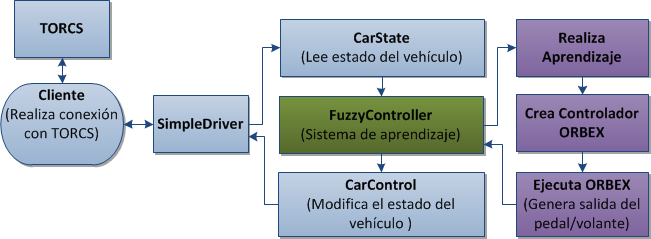
\includegraphics[width=0.6\linewidth]{figures/Diseno.png}
\caption{Esquema de ejecución de una prueba realizada con TORCS. Las clases en azul son las que vienen con TORCS, la clase verde fue la que se desarrolló y en morado se indica el funcionamiento de dicha clase}
\label{fig:esqT}
\end{figure}     

Para la automatización del pedal del automóvil, se implementó el cálculo de cinco \textbf{métricas del estado del vehículo}, las cuales se presentan en la tabla \ref{tab:metricas}, para utilizarlas como variables de entrada deben ser especificadas en el archivo de configuración.

\begin{table}[htb]
\begin{tabular}{|c|p{7.5cm}|c|}
\hline 
\rowcolor[gray]{0.9} \textbf{Métrica} & {\hspace{2.5 cm} \textbf{Descripción}} & \textbf{Formula} \\ 
\hline \hline
Error & Error de velocidad en un instante $i$ & \parbox{4cm}{\vspace{1 mm} $\gls{error} = \gls{P(i)} - \gls{V(i)}$ \vspace{0.5 mm}} \\ 
\hline 
Derivada & Rapidez con la que varia el valor del error de velocidad con respecto al tiempo & \parbox{4cm}{\vspace{1 mm}$\gls{dedt} = \frac{\gls{error}-\varepsilon_v(i-1)}{\gls{t(i)}-t(i-1)}$\vspace{0.5 mm}} \\ 
\hline 
Integral & El área bajo la curva de la función error de velocidad en los últimos diez instantes de tiempo & \parbox{5.6cm}{\vspace{1 mm}$\gls{integrall} = \gls{summod}$} \\ 
\hline 
Aceleración & Aceleración del automóvil & \parbox{4cm}{\vspace{1 mm}$\gls{a(i)} = \frac{V(i)-V(i-1)}{t(i)-t(i-1)}$\vspace{0.5 mm}} \\ 
\hline 
Perfil & Utiliza el valor del perfil de velocidad & \\ 
\hline 
\end{tabular} 
\caption{Métricas implementadas en el sistema. Donde $P(i)$ es el valor del perfil de velocidad, $V(i)$ la velocidad del carro y $t(i)$ el tiempo en el instante $i$. }
\label{tab:metricas}
\end{table}

%\begin{itemize}
%\item \textbf{Error}: error de velocidad en un instante $i$ calculado como 
%\[\gls{error} = \gls{P(i)} - \gls{V(i)}\]
%Siendo $P(i)$ el valor del perfil de velocidad en el instante $i$, y $V(i)$ la velocidad del carro en el instante $i$. 
%\item \textbf{Derivada}: rapidez con la que varia el valor del error de velocidad con respecto al tiempo:
%\[ \gls{dedt} = \frac{\gls{error}-\varepsilon_v(i-1)}{\gls{t(i)}-t(i-1)} \] 
%\item \textbf{Integral}: área bajo la curva de la función error de velocidad en los últimos diez instantes de tiempo:
%\[ \gls{integrall} = \gls{summod} \]
%\item \textbf{Aceleración}: aceleración del automóvil:
%\[ \gls{a(i)} = \frac{V(i)-V(i-1)}{t(i)-t(i-1)} \]
%\item \textbf{Perfil}: utiliza el valor del perfil de velocidad.
%\end{itemize}

El proceso cliente crea un nuevo objeto {\tt FuzzyController}, el cual se encarga tanto de todo el sistema de aprendizaje, como de la ejecución y configuración del controlador difuso definido por la librería \gls{ORBEX}. La clase {\tt FuzzyController} se inicializa con las variables mostradas en la tabla \ref{tab:fuzzycontroller}. 
%El constructor para crear una instancia de {\tt FuzzyController} es el siguiente:


\begin{table}[htb]
	\centering
		\begin{tabular}{|c|c|}
			\hline
			\rowcolor[gray]{0.9} \textbf{Campo} & \textbf{Descripción} \\ \hline \hline
			\textit{entries} & Número de entradas que se vana a pasar \\ \hline
			\textit{ets} & Número de etiquetas por cada variable de entrada \\ \hline
			\textit{rs1} & Rango inferior por cada variable de entrada \\ \hline
			\textit{rs2} & Rango superior por cada variable de entrada \\ \hline
			\textit{metrics} & Lista de métricas a utilizar \\ \hline
			\textit{ctte} & Constante de normalización (sección \ref{sec:aprendizajeL})\\ \hline
			\textit{size\_c} & Tamaño del ciclo a utilizar (sección \ref{sec:aprendizajeG}) \\ \hline
			\textit{control} & Genera un fichero de control si es verdadero \\ \hline
		\end{tabular}
		\caption{Variables utilizadas por la clase {\tt FuzzyController}.}
		\label{tab:fuzzycontroller}
\end{table}


%\begin{alltt}
%FuzzyController (
%    int entries, //número de entradas que se vana a pasar.
%    int *ets, //número de etiquetas por cada variable de entrada.
%    double *rs1, //rango inferior por cada variable de entrada.
%    double *rs2, //rango superior por cada variable de entrada.
%    string *metrics, //Lista de métricas a utilizar.
%    double ctte = 100, //Constante de normalización.
%    int size_c = 500, //Tamaño del ciclo a utilizar (sección \ref{sec:aprendizajeG}).
%    bool control = false //Genera un fichero de control si es verdadero.
%)
%\end{alltt}

{\tt FuzzyController} posee implementado el cálculo de los valores de las métricas que se definieron en el archivo de configuración, al igual que genera el archivo {\tt Controlador.ORB} que utiliza la librería \gls{ORBEX}, y \textbf{cinco archivos de salida},  presentados en la tabla \ref{tab:logs}.

\begin{table}[htb]
	\centering
\begin{tabular}{|l|p{12 cm}|}
\hline 
\rowcolor[gray]{0.9} \textbf{Nombre} & \textbf{Descripción} \\ \hline \hline
Log\_controller & Cada columna posee los valores correspondientes al estado del carro y del controlador difuso por cada iteración, como por ejemplo: el número de la iteración, valor del pedal (valor de salida de \gls{ORBEX}), velocidad y aceleración del automóvil, perfil de velocidad, variables de entrada, número de etiquetas, etc. \\ 
\hline 
Log\_etiquetas & Posee el grado de activación de las etiquetas correspondientes a las variables de entrada en cada iteración (referirse a la sección \ref{sec:orbex}) \\ 
\hline 
Log\_reglas & Posee el grado de activación de las reglas del controlador difuso en cada iteración \\ 
\hline 
Los\_singletons & Posee el valor de los singletons en cada iteración \\ 
\hline 
Log\_trapecios & Posee las coordenadas correspondientes a cada trapecio \\ 
\hline 
\end{tabular} 
\caption{Archivos de salida que se implementaron.}
\label{tab:logs}
\end{table}

%\begin{itemize}
%\item Log\_controller: en cada columna posee los valores correspondientes al estado del carro y del controlador difuso por cada iteración, como por ejemplo: el número de la iteración, valor del pedal (valor de salida de \gls{ORBEX}), velocidad y aceleración del automóvil, consigna de velocidad, variables de entrada, número de etiquetas, etc.
%\item Log\_etiquetas: posee el grado de activación de las etiquetas correspondientes a las variables de entrada en cada iteración.
%\item Log\_reglas: posee el grado de activación de las reglas del controlador difuso en cada iteración.
%\item Los\_singletons: posee el valor de los singletons en cada iteración.
%\item Log\_trapecios: posee las coordenadas correspondientes a cada trapecio.
%\end{itemize}


\section{Aprendizaje local} 
\label{sec:aprendizajeL}


El aprendizaje local consiste en \textbf{modificar los consecuentes de las reglas}, con la finalidad de que el sistema realice un seguimiento más preciso de la señal de referencia (en el caso del control de los pedales, la señal es el perfil de velocidad), y está basado en la evaluación del estado actual del automóvil y la corrección de las reglas responsables por alcanzar dicho estado. 

En la figura \ref{fig:esquemaL} se presenta un esquema del aprendizaje local de acuerdo a lo realizado en esta sección. Cuando indicamos que las acciones deben ser más altas o más bajas, significa que el impacto que generan las reglas que se activaron en la salida del pedal, no generan el comportamiento deseado, por lo que se deben aumentar o disminuir, según sea el caso, los singletons de dichas reglas. Nos referimos a que las acciones son adecuadas, cuando el controlador logra mantener el error de velocidad en cero, o cuando el controlador, logra que el error de velocidad vaya creciendo o reduciéndose para alcanzar al cero, mientras la aceleración del vehículo se encuentra en un rango establecido. 

\begin{figure}[!htb]
\centering
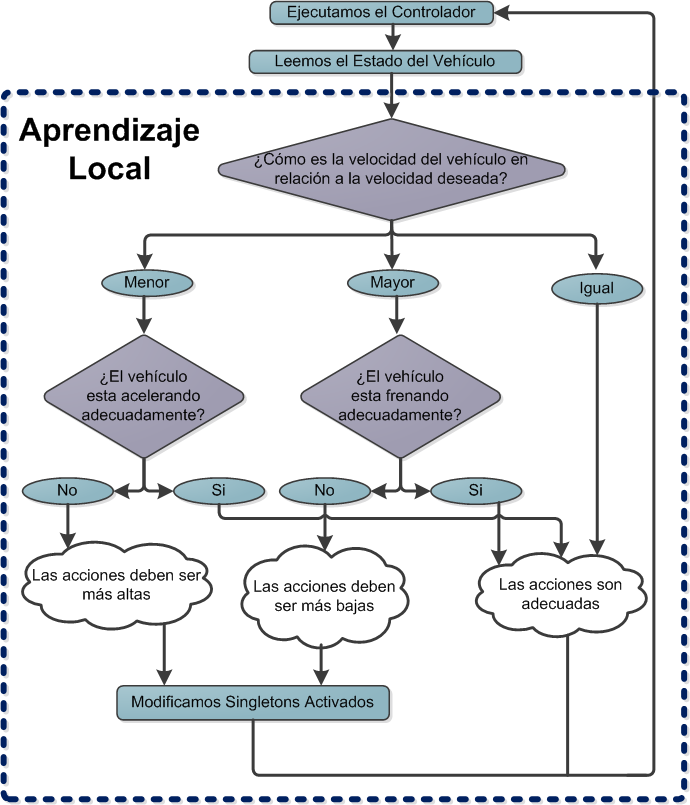
\includegraphics[width=0.75\linewidth, height= 10 cm]{figures/EsquemaLocal.png}
\caption{Esquema de funcionamiento de aprendizaje local.}
\label{fig:esquemaL}
\end{figure}  

Suponiendo una iteración del controlador, en el instante $t-1$ con un valor de referencia $P(t-1)$ (velocidad que se desea alcanzar) se obtiene un valor para el pedal. Al aplicarse dicho valor al carro, se alcanza la velocidad $V(t)$, en el caso de que $V(t) < P(t-1)$ significa que el valor del pedal para el instante $t$, debió haber sido mayor, de igual manera si $V(t) > P(t-1)$ implica que el valor del pedal fue demasiado elevado. En ambos casos, se debe corregir únicamente, los singletons correspondientes a aquellas reglas que se activaron para obtener el valor de salida del pedal, ya que son las responsables de que el vehículo alcanzara ese estado. La modificación de los singletons viene dada por la siguiente expresión:

\begin{equation}\label{eq:single}
\gls{s(t)} = s(t-1) + \frac{P(t-1)-V(t)}{\gls{Cte}}*\gls{mu_{i}(t-1)}
\end{equation}

\noindent, donde $s(t-1)$ es el valor del singleton en el instante $t-1$, $\mu_{i}(t-1)$ es el grado de activación de la regla $i$ en el instante $t-1$ y $Cte$ es una constante de normalización previamente definida. 

En todas las pruebas que se realizaron, los singletons fueron inicializados en cero, sin embargo el sistema puede utilizarse para ajustar los singletons de las reglas que utilicen controladores que hayan sido previamente configurados, bien sea por el mismo sistema de aprendizaje, o a partir de maquinas de aprendizaje que realicen un aprendizaje supervisado.


\subsection{Elección de la constante de normalización}


Se realizaron simulaciones en las cuales se probaron distintos valores de la constante de normalización, y fueron variándose el número de etiquetas por entrada, con la finalidad de elegir un valor adecuado para la constante. Como variables de entrada se utilizaron el error y la derivada del error, en los rangos [-25,25] y [-8,8] respectivamente, las funciones de pertenencia de cada variable de entrada se variaron desde 2 hasta 7 en cada corrida, los valores de constante utilizados fueron 50, 100 y 150. 

\begin{figure}[htb]
\centering
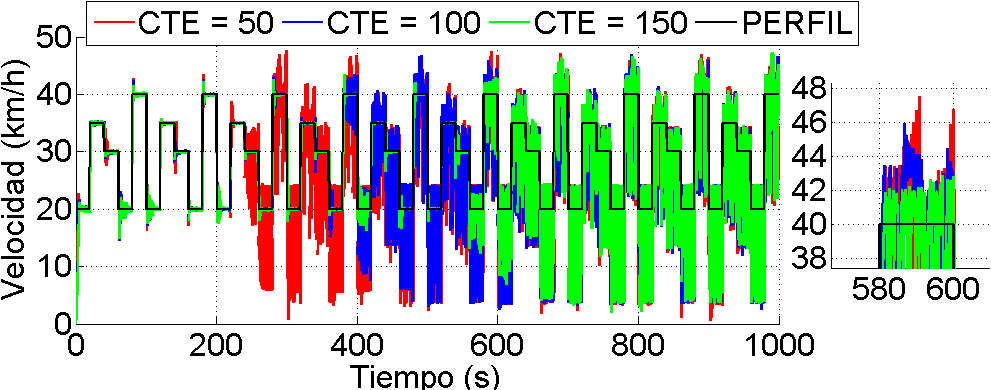
\includegraphics[width=0.6\linewidth,type=png,ext=.png,read=.png]{figures/tresC}
\caption{Comparación de simulaciones con distintos valores de la constante, utilizando 5 etiquetas por variable de entrada.}
\label{fig:tresC}
\end{figure} 



Al analizar los resultados de las distintas simulaciones, \textbf{se decidió por utilizar 100} como valor para la constante de normalización, en la figura \ref{fig:tresC}, se observa que entre 100 y 150, la diferencia no es tan notable, mientras que con 50 se observan oscilaciones muy grandes de la velocidad. Utilizar un valor como 50 o más pequeño resultaría en modificaciones muy grandes a los singletons, lo cual dificultaría las tareas de ajustes de algunas magnitudes como la aceleración, en cambio a medida que se va aumentando el valor de la constante de normalización, se va haciendo más lento el proceso de aprendizaje, debido a que se van haciendo más pequeños las modificaciones a los singletons, necesitando una cantidad mayor de ejecuciones del sistema para alcanzar una configuración aceptable.

Las grandes oscilaciones que se observan en la figura \ref{fig:tresC} un poco antes del segundo 400, se pensó que ocurrían debido a que los singletons se modificaban en cada iteración, y que se llegaba a un punto en el cual los cambios eran sencillamente muy grandes, por lo que obteníamos unos valores muy extremos para el pedal.


%\begin{figure}[htb]
%\centering
%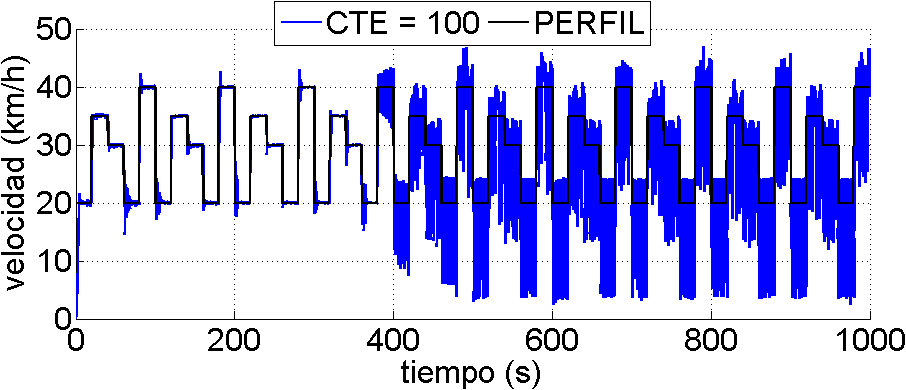
\includegraphics[width=0.8\linewidth,type=png,ext=.png,read=.png]{figures/ctte100}
%\caption{Simulación con el valor de la constante elegida.}
%\label{fig:ctte100}
%\end{figure} 

\subsection{Condicionamiento de la modificación de singletons}
\label{subsec:condicionamiento}


Con la finalidad de variar el valor de los singletons lo menos posible, se condicionó esta acción. Se establecieron \textbf{dos casos formados por tres reglas cada uno}, si ninguno de los dos se cumple, modificamos los singletons. Los casos se presentan a continuación:



\begin{itemize}
\item Caso 1: $V(i) < P(i)$, $a(i) > 0$ y $a(i) < \gls{a_c}+2$.
%\begin{itemize}
%\item $V(i) < P(i)$ : la velocidad del automóvil es menor a la velocidad que queremos alcanzar.
%\item $a(i) > 0$ : la aceleración del automóvil es positiva.
%\item $a(i) < a_c+2$ : la aceleración del automóvil es menor a la aceleración de confort más dos.
%\end{itemize}
\item Caso 2: $V(i) > P(i)$, $a(i) < 0$ y $a(i) > -a_c - 2$.
%\begin{itemize}
%\item $V(i) > P(i)$ : la velocidad del automóvil es mayor a la velocidad que queremos alcanzar.
%\item $a(i) < 0$ : la aceleración del automóvil es negativa.
%\item $a(i) > -a_c - 2$ : la aceleración del automóvil es mayor al negativo de la aceleración de confort menos dos.
%\end{itemize}
\end{itemize}

El \textit{Caso 1} representa la situación en que la velocidad del automóvil es menor a la velocidad que se desea alcanzar, la aceleración del automóvil es positiva y la aceleración del automóvil es menor a la aceleración de confort más dos. Mientras que el \textit{Caso 2} representa la situación especular. 

\textbf{La aceleración de confort} ($a_c$), es aquella a partir de la cual el cambio de velocidad genera una sensación desagradable en las personas. Se utilizó un valor de 8 km/h/s como aceleración de confort. El propósito del condicionamiento, es llegar a un punto en el cual se alcance el aprendizaje necesario, para poder procesar cualquier perfil de velocidad sin realizar modificaciones bruscas a los singletons.

\begin{figure}[htb]
\centering
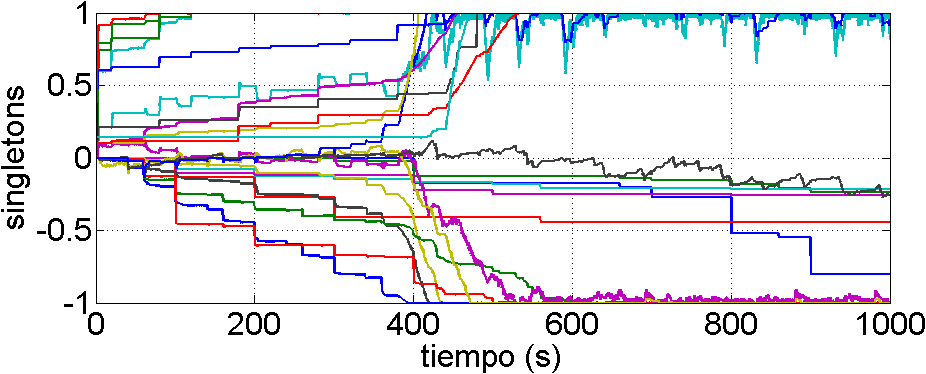
\includegraphics[width=0.5\linewidth,type=png,ext=.png,read=.png]{figures/421single1}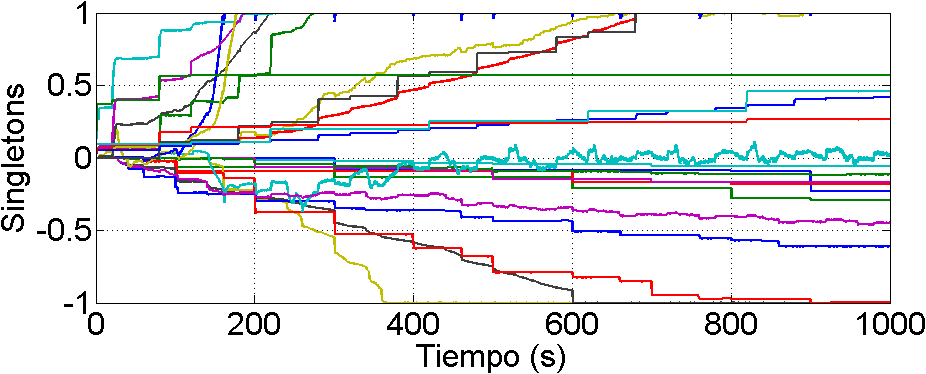
\includegraphics[width=0.5\linewidth,type=png,ext=.png,read=.png]{figures/421single2}
\caption{Singletons sin el condicionamiento (izquierda) y con el condicionamiento (derecha). Cada línea de color representa el valor de los singleton (consecuente de las reglas) a lo largo de la ejecución.}
\label{fig:421single2}
\end{figure} 

En la figura \ref{fig:421single2} se puede ver cómo varían los singletons en una ejecución del aprendizaje sin utilizar el condicionamiento de aceleración (izquierda) y utilizándolo (derecha). Cuando no se utiliza el condicionamiento algunos singletons son modificados repetidamente en pequeños espacios de tiempo, lo que resulta en oscilaciones cortas en las líneas que los representan; en cambio, cuando es utilizado se obtienen líneas más suaves, ya que al momento de modificarse los singletons se realizan principalmente uno o dos cambios seguidos.

Tratando de adecuar la aceleración del automóvil, para evitar un comportamiento violento, se hizo un \textbf{nuevo ajuste} luego de aplicada la fórmula de modificación de singletons. En caso de que la aceleración sea mayor a la aceleración de confort, se resta al singleton el 10\% del grado de activación que tuvo, mientras que si es menor al negativo de la aceleración de confort, se suma 10\% del grado de activación. Como el rango de los singletons es [-1,1], se debe garantizar que los valores se encuentren contenidos en él. 

Con este método se realizaron diversas simulaciones, para las cuales se utilizaron el valor de constante seleccionado anteriormente ($Cte=100$) y dos valores de entrada (\textit{error} y \textit{derivada}), a los que se les fueron variando sus respectivos números de etiquetas en cada prueba. En todas las pruebas se encontró el comportamiento que se presenta en la figura \ref{fig:loco100}, correspondiente a una simulación con cinco etiquetas por cada entrada.

\begin{figure}[htb]
\centering
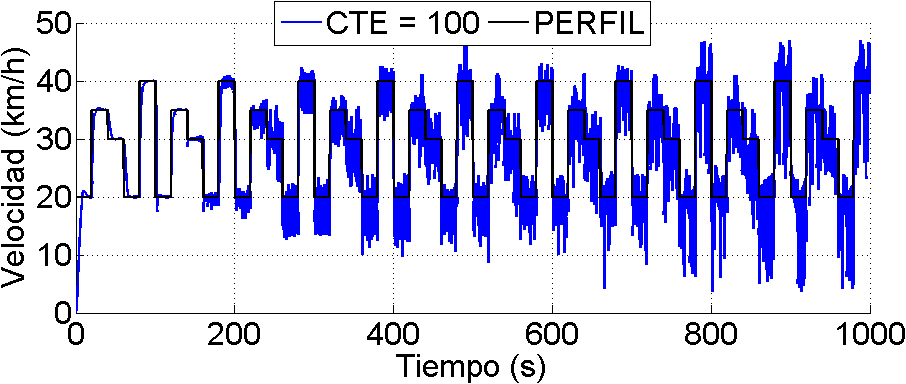
\includegraphics[width=0.6\linewidth,type=png,ext=.png,read=.png]{figures/loco100}
\caption{Simulación con el condicionamiento de singletons implementado.}
\label{fig:loco100}
\end{figure} 

Al ver que el problema de las oscilaciones grandes no se resolvía con el condicionamiento de la modificación de singletons, se hizo un análisis de la estructura del programa y la formulación del problema. Se encontró que el error se produce porque \textbf{la variación de singletons se realiza tras ejecutar el controlador \gls{ORBEX}}, y no luego de pasar el valor del pedal al carro y recibir los valores actualizados del estado del vehículo, por lo que se realizaban todos los cálculos y comparaciones, utilizando los valores de aceleración y velocidad correspondientes a la iteración anterior.

Al realizar la corrección de los consecuentes justo después de ejecutarse el controlador no se estaba aplicando la expresión \ref{eq:single}, sino que realmente se aplicaba la siguiente:
\[ s(t) = s(t-1) + \frac{P(t-1)-V(t-1)}{C}*\mu_{i}(t-1)\]

Como se aprecia en la figura \ref{fig:buenoCtte100}, al \textbf{reestructurar el código} para que se realizaran las modificaciones a los singletons luego de que se aplicara el nuevo valor del pedal, de forma tal que la formula utilice el valor de velocidad correspondiente, se eliminaron las oscilaciones bruscas que ocurren un poco antes del instante 400, y se observa un comportamiento más sutil.

\begin{figure}[htb]
\centering
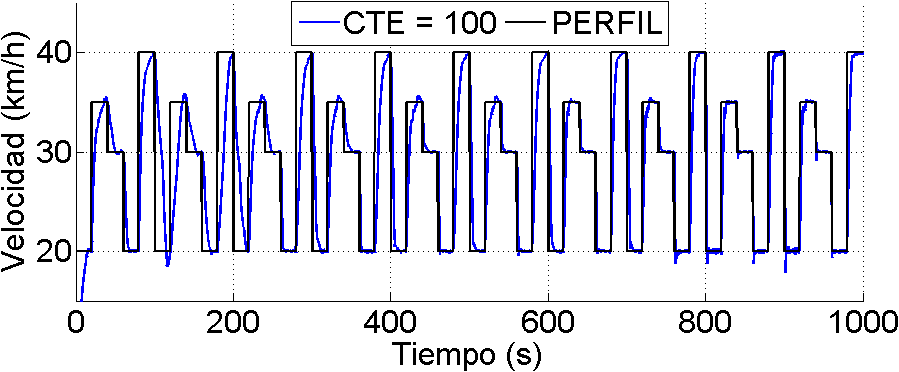
\includegraphics[width=0.6\linewidth,type=png,ext=.png,read=.png]{figures/buenoCtte100}
\caption{Simulación con reestructuración del código de modificación.}
\label{fig:buenoCtte100}
\end{figure} 

Durante la ejecución de las simulaciones se obtuvieron valores de aceleración muy por encima de lo adecuado, pero se decidió implementar primero el aprendizaje global, antes que buscar maneras para mejorar los valores desde la etapa local, esperando obtener mejoras con la implementación de la nueva etapa.


\section{Aprendizaje global}
\label{sec:aprendizajeG}

En esta etapa, el objetivo es evaluar el comportamiento que ha mostrado el controlador, y decidir si es necesario \textbf{modificar la topología} del mismo, ya sea modificando la posición de la base superior de los trapecios, o insertando etiquetas o funciones de pertenencia nuevas. En la figura \ref{fig:esquemaG}, se presenta un esquema con el aprendizaje global, de acuerdo a lo realizado en esta sección.

\begin{figure}[!htb]
\centering
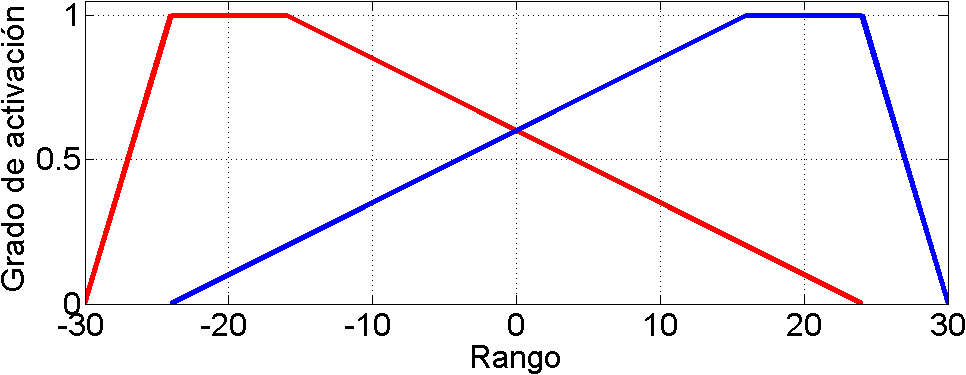
\includegraphics[width=0.35\linewidth]{figures/2.png} \hspace{0.5cm} 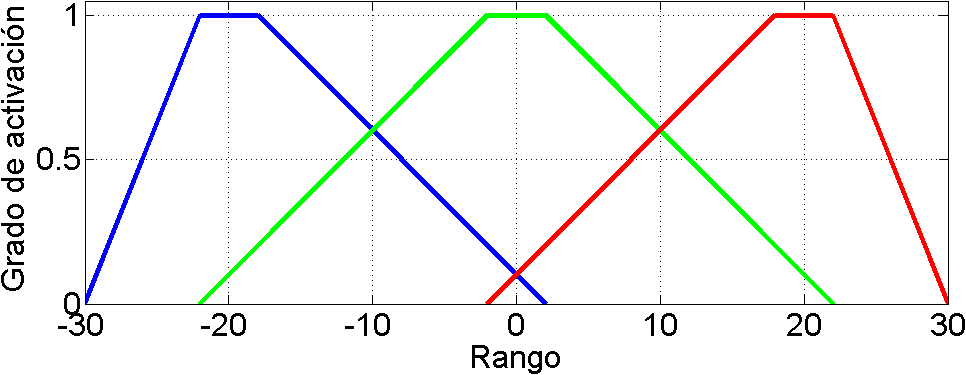
\includegraphics[width=0.35\linewidth]{figures/3.png}
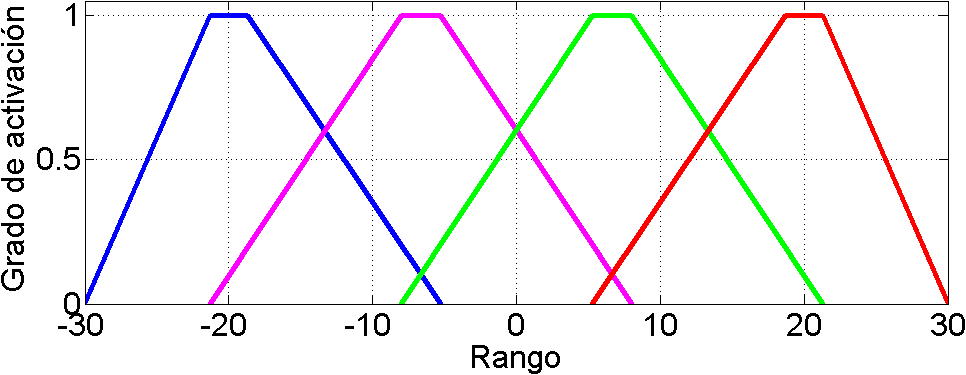
\includegraphics[width=0.35\linewidth]{figures/4.png} \hspace{0.5cm} 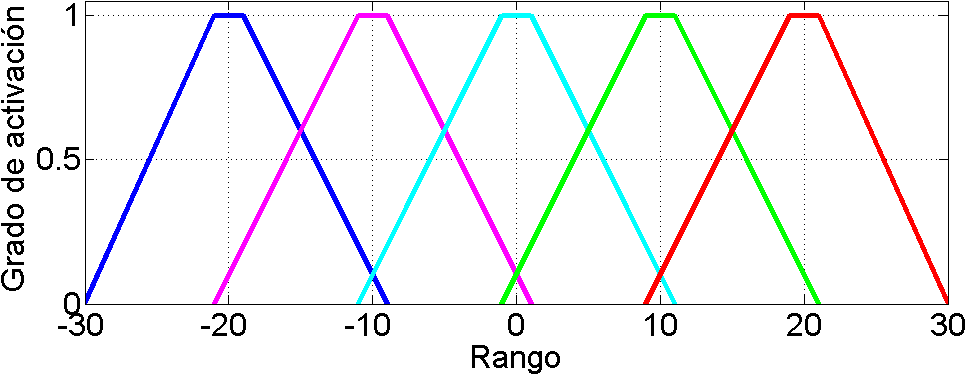
\includegraphics[width=0.35\linewidth]{figures/5.png}
\caption{Topología de un controlador, que utiliza funciones de pertenencia o etiquetas, con forma trapezoidal, igualmente distribuidas en un rango de [-20,20], con dos etiquetas (arriba izquierda), con tres etiquetas (arriba derecha), con cuatro etiquetas (abajo izquierda) y con cinco etiquetas (abajo derecha)}
\label{fig:trapeciosD}
\end{figure} 

El sistema se diseñó para trabajar con trapecios igualmente distribuidos, cada vez que se va a insertar una nueva etiqueta a alguna variable de entrada, se genera el nuevo grupo de trapecios y se colocan a lo largo del rango de la variable, como se aprecia en la figura \ref{fig:trapeciosD}. Los trapecios están colocados de manera que se pueda garantizar que cualquier valor de entrada estará cubierto como mínimo por dos trapecios.

\begin{figure}[!htb]
\centering
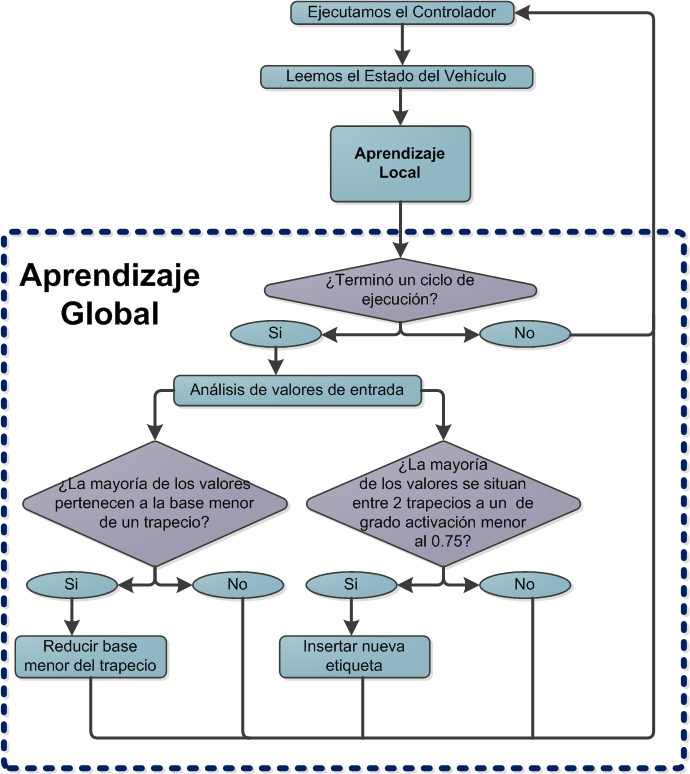
\includegraphics[width=0.75\linewidth, height = 10 cm]{figures/EsquemaGlobal.png}
\caption{Esquema de funcionamiento de aprendizaje global.}
\label{fig:esquemaG}
\end{figure} 

Se comienza el aprendizaje global dividiendo el rango de cada variable de entrada entre la mitad del tamaño de la base menor de un trapecio, de tal manera que la base menor de cada trapecio este cubierta por lo menos por dos subrangos. En caso que el número de subrangos que se generan de la división es par, se aumenta dicho número en uno, ya que si dividimos entre un número impar, garantizamos tener un subrango en cual el punto medio sea el cero.

Cada vez que se ejecuta el controlador, se busca a que subrango pertenecen los valores de entrada, y se aumenta en uno un contador que corresponde al número de valores de entrada que han pertenecido a dicho subrango. 

Se define un \textbf{ciclo de ejecución} como la evaluación de un cierto número de iteraciones del controlador, el tamaño de estos se especifica en la variable \textit{size\_c} del constructor de la clase \textit{FuzzyController}. Cada vez que se termina un ciclo, se ejecuta la etapa de aprendizaje global, se comienza por determinar cuáles son los dos subrangos con mayor valor en su contador. Utilizando el punto medio de los dos subrangos, se busca a cuales trapecios pertenecen y se determina si se encuentran en alguno de estos dos casos:

\begin{itemize}
\item Ambos puntos pertenecen a la base menor del mismo trapecio.
\item Ambos puntos pertenecen al mismo lado del trapecio, y se encuentran a un nivel de activación menor al 75\%
\end{itemize} 

En caso de pertenecer a la base menor del mismo trapecio, \textbf{se reduce la base menor}  de dicho trapecio en un 80\% y se reinician los contadores de los subrangos. Al reducir la base menor, se evita que la gran mayoría de los valores de entrada posean el mismo grado de activación, obteniendo un controlador más específicos. 

\begin{figure}[htb]
\centering
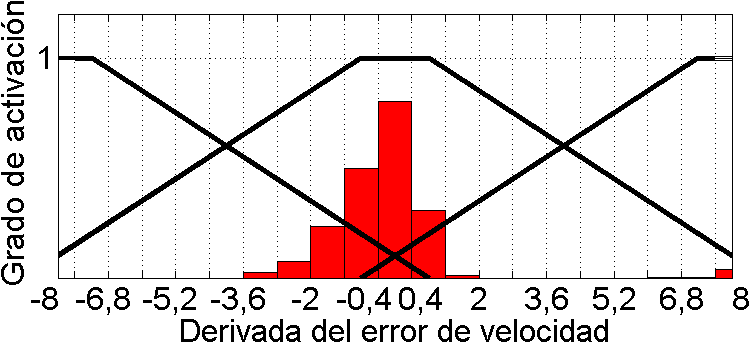
\includegraphics[width=0.45\linewidth,type=png,ext=.png,read=.png]{figures/label11}\hspace{0.5cm} 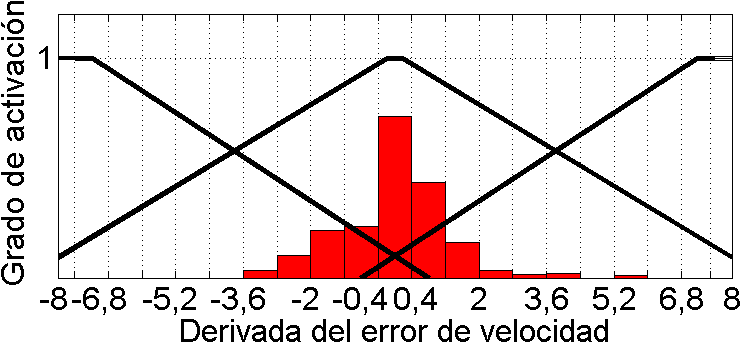
\includegraphics[width=0.45\linewidth,type=png,ext=.png,read=.png]{figures/label12}
\caption{Histograma del error de velocidad obtenido en un ciclo, con sus respectivas funciones de pertenencia antes de realizar el ajuste global (izquierda) y tras realizar el ajuste global (derecha).}
\label{fig:label11}
\end{figure} 

En la figura \ref{fig:label11} (izquierda) se puede observar que la gran mayoría de los valores de entrada obtenidos de la derivada del error en un ciclo, se encuentran alrededor del cero, y dada la manera en la que están distribuidos los trapecios, ese rango de valores pertenecen a la base menor del trapecio ubicado en el medio. De acuerdo a las reglas colocadas, se debe reducir la base en un 80\%, como se aprecia en la figura \ref{fig:label11} (derecha), correspondiente al ciclo de ejecución siguiente.

%\begin{figure}[htb]
%\centering
%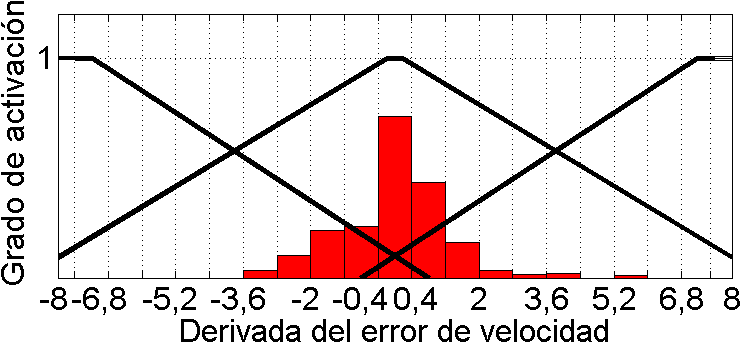
\includegraphics[width=0.8\linewidth,type=png,ext=.png,read=.png]{figures/label12}
%\caption{Topología luego de la reducción de la base menor del trapecio ubicado en el medio.}
%\label{fig:label12}
%\end{figure} 

Si ambos puntos se encuentran en el mismo lado del trapecio y a un nivel de activación menor al 75\%, se procede a \textbf{insertar un nueva función de pertenencia} de la siguiente manera: se genera la nueva cantidad de trapecios uniformemente distribuidos para esa entrada, se actualiza el número de etiquetas y se recalculan el número de reglas, subrangos, singletons, asignándole cero a estos últimos. 

\begin{figure}[h]
\centering
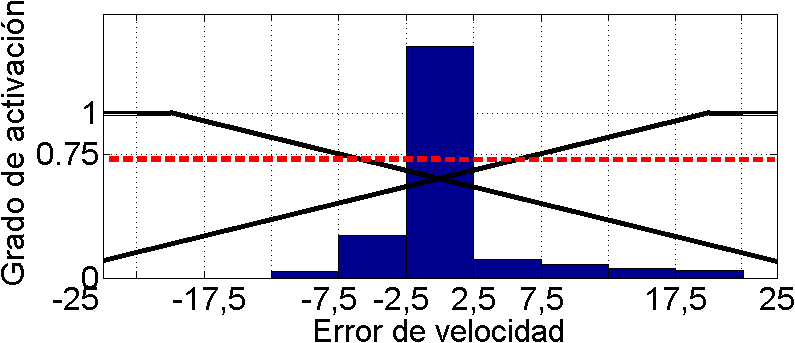
\includegraphics[width=0.45\linewidth,type=png,ext=.png,read=.png]{figures/label21}\hspace{0.5cm} 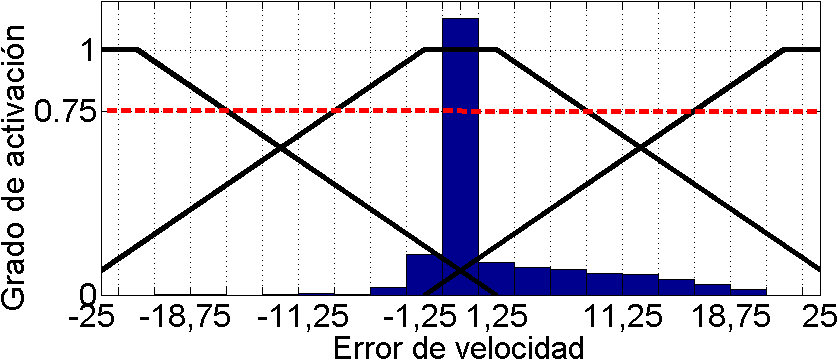
\includegraphics[width=0.45\linewidth,type=png,ext=.png,read=.png]{figures/label22}
\caption{Histograma de la derivada del error en un ciclo, con sus respectivas funciones de pertenencia antes de realizar el ajuste global (izquierda) y tras el ajuste global (derecha).}
\label{fig:label21}
\end{figure} 

El caso en el cual se inserta una nueva función de pertenencia, se puede apreciar en la figura \ref{fig:label21} (izquierda). Los dos subrangos con mayor número de elementos, se encuentran a un nivel de activación menor al 75\%, por lo que se agrega una función de pertenencia nueva y se recalculan los trapecios asociados a dichas funciones, para la ejecución del ciclo siguiente, como se ve en la figura \ref{fig:label21} (derecha). 

%\begin{figure}[h]
%\centering
%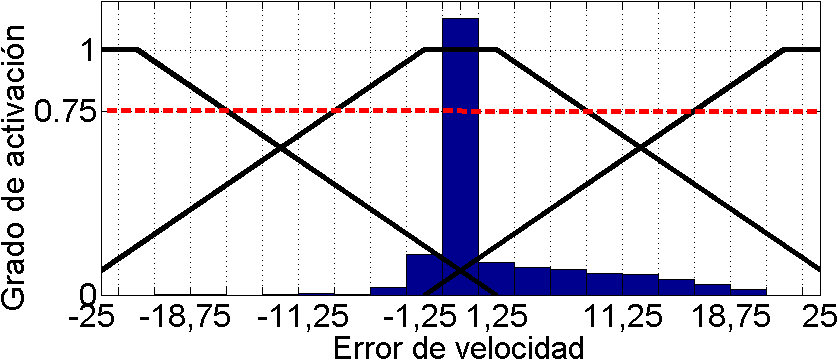
\includegraphics[width=0.8\linewidth,type=png,ext=.png,read=.png]{figures/label22}
%\caption{Topología luego de la inserción de una nueva función de pertenencia.}
%\label{fig:label22}
%\end{figure} 



\section{Ajuste de la aceleración}
\label{sec:ajuste}

En las simulaciones realizadas, se encontró que el vehículo alcanzaba unos niveles de aceleración (tanto positiva como negativa) muy por encima de lo deseable, resultado de los elevados valores que se transmitían al pedal a la hora de encontrarse con un cambio en el perfil de velocidad. Esta situación ocurría ya que el controlador buscaba alcanzar el nuevo valor con la mayor rapidez posible, de manera que el error de velocidad se vuelva cero. 

Ésto se ilustra en la figura \ref{fig:frenaso}, donde se muestra la aceleración obtenida por el vehículo en una de las simulaciones. En ella puede verse que en el instante 400, momento cuando termina el cuarto ciclo (cada ciclo dura 100 segundos, sección \ref{subsec:diseno}) y ocurre el cambio de 40 km/h a 20 km/h, la aceleración sobrepasa el valor de -10 km/h/s, que es el límite aceptable establecido para esta magnitud. A partir de ese momento, se evidencia un aumento muy brusco a la hora de terminar los ciclos, dado que el controlador, para reducir rápidamente la velocidad, manda una señal muy fuerte al pedal. En los primeros tres ciclos no se evidencia este fenómeno, ya que en estos ciclos se realizan las modificaciones a la topología del controlador, que finalizan con la reinicialización de los singletons. 

\begin{figure}[h]
\centering
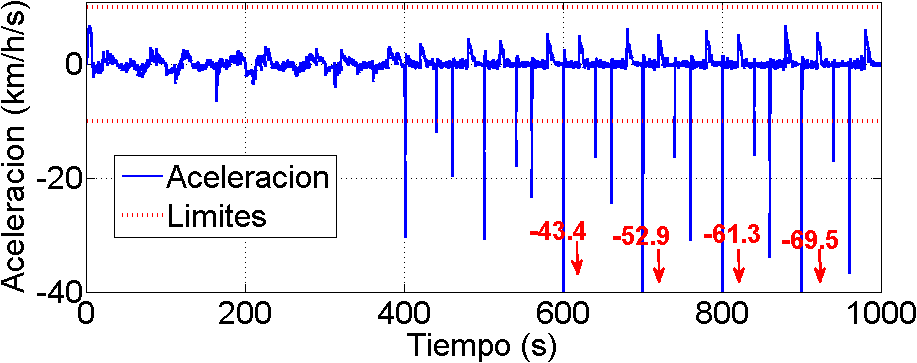
\includegraphics[width=0.6\linewidth,type=png,ext=.png,read=.png]{figures/frenaso}
\caption{Aceleración del vehículo.}
\label{fig:frenaso}
\end{figure} 

Para ajustar el cambio de aceleración, se modificó la etapa de aprendizaje local, y se agregó unos cambios correspondientes al comportamiento de los pedales del vehículo, los cuales se explican en las secciones \ref{subsec:ajusteS} y \ref{sec:ajusteP} respectivamente. En la figura \ref{fig:esquemaA} se presenta un esquema de como queda el sistema de aprendizaje, luego de aplicarse los nuevos ajustes.  

\begin{figure}[htb]
\centering
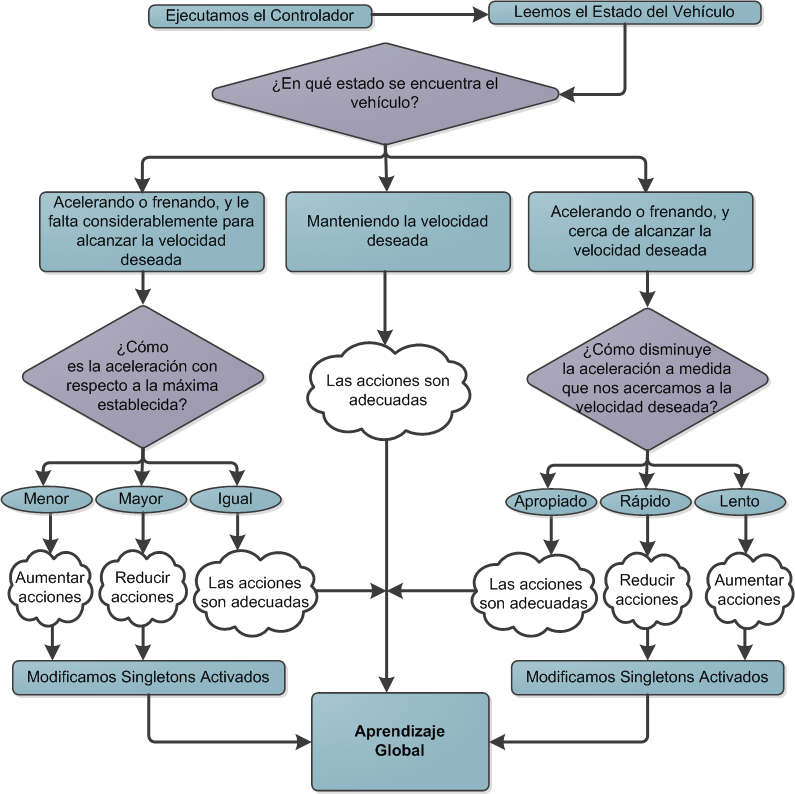
\includegraphics[width=0.85\linewidth,height = 10 cm]{figures/EsquemaAjustes.png}
\caption{Esquema de funcionamiento de aprendizaje local luego de los ajustes.}
\label{fig:esquemaA}
\end{figure}

\subsection{Ajuste a la modificación de singletons}
\label{subsec:ajusteS}


En la sección \ref{subsec:condicionamiento}, se establecieron dos condiciones para que se realice la \textbf{modificación de los singletons} y poder controlar mejor el comportamiento del automóvil, las cuales se cambiaron por unas más específicas. Se identificaron varias situaciones para las cuales se van a realizar dichas modificaciones.

\textbf{Si el error de velocidad es positivo ($velocidad<perfil$)} se debe acelerar para alcanzar la nueva consigna. Dependiendo de qué tan cerca se encuentra de alcanzar la velocidad deseada, se definen dos casos.

\begin{enumerate}
\item Si el error de velocidad es mayor al valor de la aceleración de confort ($\gls{error}>a_c$); el automóvil se encuentra en un estado favorable para alcanzar la aceleración máxima establecida. Tomando esto en consideración, la modificación de los singletons se establece según:
\begin{itemize}
\item $a(i) > a_c +2$ : el automóvil sobrepasó la aceleración máxima, por lo que se realiza una disminución al valor de los singletons, que viene dada por la siguiente expresión:
\begin{equation}\label{eq:sinMenos}
s(t) = s(t-1) - \frac{P(t-1)-V(t)}{C}*\mu_{i}(t-1)
\end{equation}
\item $a(i) < a_c -2$ : el automóvil no ha alcanzado la aceleración máxima, por lo que se realiza un aumento al valor de los singletons, el cual viene dado por:
\begin{equation}\label{eq:sinMas}
s(t) = s(t-1) + \frac{P(t-1)-V(t)}{C}*\mu_{i}(t-1)
\end{equation}
\item Si no se cumple ninguna de las condiciones anteriores, es decir, la aceleración del carro se encuentra en el intervalo [$a_c -2$,$a_c +2$], el vehículo se encuentra en el punto óptimo de aceleración, en el que no se realizan modificaciones.
\end{itemize}
 

\item En el caso donde $\gls{error} \leq a_c$, el carro debe ir disminuyendo progresivamente la aceleración a medida que se alcanza el valor de la consigna. De la misma manera como ocurre en el caso anterior:

\begin{itemize}
\item $a(i) > \gls{error}+2$ : el automóvil no ha disminuido lo suficiente la aceleración, por lo que se realiza una disminución al valor de los singletons, que viene dada por la expresión (\ref{eq:sinMenos}).
\item $a(i) < max(0,\gls{error}-2)$ : el automóvil ha disminuido demasiado la aceleración, por lo que se realiza un aumento al valor de los singletons, el cual viene dado por la expresión (\ref{eq:sinMas}). Se utiliza el máximo entre $0$ y $\gls{error}-2$, debido a que si se encuentra que $\gls{error}-2 < 0$, no se puede permitir que el automóvil tenga una velocidad menor que la deseada y se encuentre frenando, en este caso el rango que se permite de aceleración para el cual no se modifican los singletons queda de la siguiente manera [$0$, $\gls{error}+2$].

\item A medida que disminuye el error de velocidad, se deja un rango para la aceleración de [$\gls{error}-2$, $\gls{error}+2$], en el cual no se modifican los singletons.
\end{itemize}

\end{enumerate}


 
\textbf{Cuando el error de velocidad es negativo}, el vehículo debe frenar, se mantiene el mismo planteamiento que se utiliza en el caso anterior, ya que los casos que se presentan son análogos.

\begin{enumerate}
\item Si $\gls{error}<-a_c$, se busca alcanzar la aceleración negativa máxima, para lo cual se divide el problema en:
\begin{itemize}
\item $a(i) < -a_c -2$ : el automóvil está frenando demasiado, por lo que se realiza un ajuste a los singletons, dado por (\ref{eq:sinMenos}).
\item $a(i) > -a_c +2$ : el automóvil no desacelera lo suficiente, por lo que se aplica la expresión (\ref{eq:sinMas}) para ajustar los singletons.
\item Si no se cumple ninguna de las condiciones, los singletons no se modifican.
\end{itemize}


\item De igual manera que en el caso anterior, si $\gls{error} \geq -a_c$, se divide el problema en dos:
\begin{itemize}
\item $a(i) < \gls{error}-2$ : el automóvil sigue frenando muy fuerte, por lo que se realiza una disminución al valor de los singletons, que viene dada por la expresión (\ref{eq:sinMenos}).
\item $a(i) > min(0,\gls{error}+2)$ : el automóvil no disminuye la aceleración como se espera, por lo que se realiza un aumento al valor de los singletons, el cual viene dado por la expresión (\ref{eq:sinMas}). En este caso se utiliza el mínimo entre $0$ y $\gls{error}+2$, para evitar estar en una situación donde no se modifiquen los consecuentes, y se espera que el carro este frenando, pero en realidad se encuentre acelerando.
\item Nuevamente, si no se cumple ninguna de las condiciones, los singletons no se modifican.
\end{itemize}

\end{enumerate}


%En el cuadro \ref{tab:casosS} se presentan los casos de manera resumida.
%
%\begin{table}[htb]
%\centering
%\begin{tabular}{|p{2.5cm} | p{4.5cm} | p{4.5cm} | p{3cm} |}
%\hline
%\rowcolor[gray]{0.9} Caso 1   & $a(i)< a_c-2$              & $a(i) \in [ a_c-2$,$a_c+2]$ & $a(i) > a_c+2$ \\ \hline
%$ \varepsilon_v(i) > a_c $ & Expresión: (\ref{eq:sinMas}) & No se modifica & Expresión: (\ref{eq:sinMenos}) \\ \hline  \hline
%
%\rowcolor[gray]{0.9} Caso 2& $a(i)< max(0,\varepsilon_v(i)-2)$ & $a(i) \in [ \varepsilon_v(i)-2$,$\varepsilon_v(i)+2]$ & $a(i) > \varepsilon_v(i)+2)$ \\ \hline
%$ \varepsilon_v(i) \in [0$,$a_c] $ & Expresión: (\ref{eq:sinMas}) & No se modifica & Expresión: (\ref{eq:sinMenos}) \\ \hline \hline
%
%\rowcolor[gray]{0.9} Caso 3 & $a(i)< -a_c-2$              & $a(i) \in [ -a_c-2$,$-a_c+2]$ & $a(i) > -a_c+2$ \\ \hline
%$ \varepsilon_v(i) > -a_c $ & Expresión: (\ref{eq:sinMas}) & No se modifica & Expresión: (\ref{eq:sinMenos}) \\ \hline \hline
%
%\rowcolor[gray]{0.9} Caso 4& $a(i)< \varepsilon_v(i)-2$ & $a(i) \in [ \varepsilon_v(i)-2$,$\varepsilon_v(i)+2]$ & \raggedright $a(i)> $ $min( \varepsilon_v(i)+2)$,$0]$ \tabularnewline
% \hline
%$ \varepsilon_v(i)$ $\in [-a_c$,$0] $ & Expresión: (\ref{eq:sinMas}) & No se modifica & Expresión: (\ref{eq:sinMenos}) \\ \hline  
%
%\end{tabular}
%\caption{Casos correspondientes a la modificación de singletons}
%\label{tab:casosS}
%\end{table}

Este enfoque más específico permite mantener un control más delicado a la hora de cambiar la velocidad. Se busca imitar la forma de conducir de las personas, las cuales no aceleran a fondo hasta llegar a la velocidad que desean, si no que pisan el pedal hasta lograr una aceleración adecuada, y a medida que se van acercando a la velocidad a la que quieren llegar, sueltan lentamente el pedal del acelerador, para no sobrepasarse.


\begin{figure}[h]
\centering
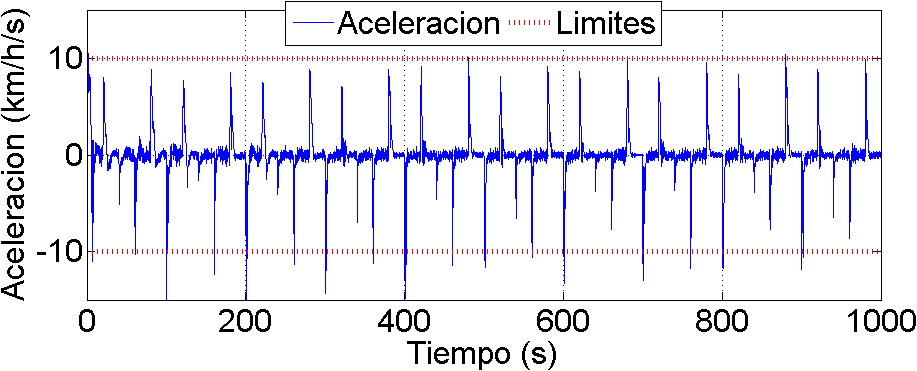
\includegraphics[width=0.6\linewidth,type=png,ext=.png,read=.png]{figures/freno4c}
\caption{Aceleración del vehículo, con el nuevo enfoque de modificación de singletons.}
\label{fig:freno4c}
\end{figure} 


En la figura \ref{fig:freno4c} se observa como la aceleración positiva alcanzó el máximo cuando le tocaba conseguir velocidades superiores, sobrepasando el límite solo en dos ocasiones, llegando a 10.42 km/h/s y 10.09 km/h/s, que son valores aceptables y no representan un problema mayor. 

Con respecto a los momentos donde se debía frenar, se logró reducir considerablemente los valores que se alcanzaban, aunque seguía sobrepasando el límite establecido, el mínimo al que llegó fue -21.80 km/h/s. Utilizando el otro enfoque, el mínimo que se alcanzó fue de -69.47 km/h/s y el comportamiento que presentó el controlador, indicaba que en el ciclo siguiente iba a ser mayor, mientras que en el nuevo, el mínimo se alcanzó en el segundo ciclo, cuando el controlador está realizando los ajustes a la topología, a partir de ese punto, a medida que avanza el aprendizaje, se fueron disminuyendo poco a poco los mínimos de aceleración.


\subsection{Ajustes del pedal}
\label{sec:ajusteP}


Cuando el valor de salida del controlador, que corresponde al pedal del controlador, cambia de signo, dependiendo del signo al que cambie, implica que \textbf{se cambió entre el pedal de aceleración y el de freno}. Este cambio no puede ser instantáneo, no se puede pasar de un valor positivo (acelerar) inmediatamente a uno negativo (frenar), ya que el objetivo es imitar la manera de conducir de las personas, por lo que se debe soltar completamente el pedal que se está utilizando, y luego presionar el otro. 

Tomando en cuenta este comportamiento, si se encuentra un cambio de signo en la salida del controlador, \textbf{se devuelve cero} como salida del pedal durante las iteraciones correspondientes a el cambio de pedal. Es importante no realizar ajuste a los singletons durante este tiempo, ya que el resultado que se devuelve y los valores obtenidos con esa salida, no corresponden a los singletons utilizados. Se establecieron tres iteraciones con salida cero para imitar el cambio de pedal.


En la figura \ref{fig:pedal002}, se observa un periodo de tiempo en el cual el carro debe frenar porque está pasando de 40 km/h a 20 km/h. Sin embargo se nota que hay dos instantes en los que el pedal pasa al lado positivo. Analizando el valor que adopta el pedal en estos dos instantes, se puede decir que son casi insignificantes, pero representan un comportamiento que no queremos que adopte el carro. No tiene sentido que mientras se esta frenando, se suelte el pedal correspondiente al freno, para pisar casi de manera imperceptible al acelerador, e inmediatamente continuar frenando. 

\begin{figure}[h]
\centering
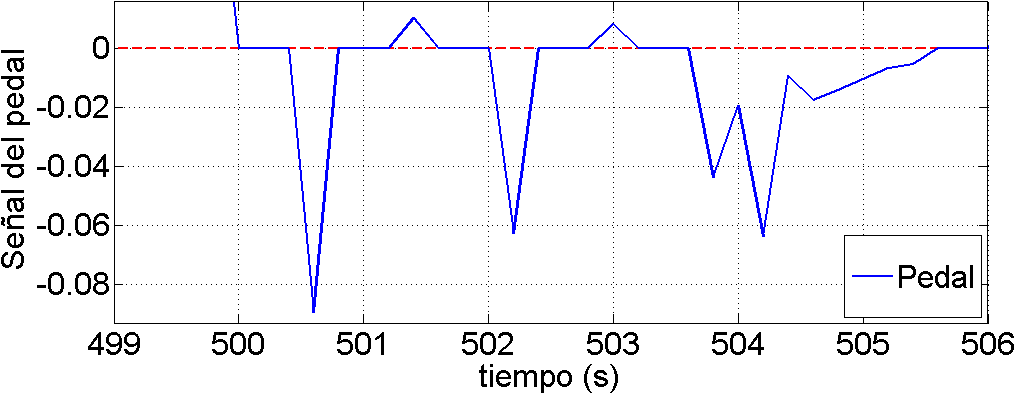
\includegraphics[width=0.6\linewidth,type=png,ext=.png,read=.png]{figures/pedal002}
\caption{Valores del pedal al pasar de 40 km/h a 20 km/h.}
\label{fig:pedal002}
\end{figure} 

Cuando se encuentren valores del pedal cuyo valor absoluto sea menor a 0.02, se retorna cero, ya que es un rango tan pequeño que los valores pertenecientes a él no inducen grandes cambios en el automóvil, y de esta forma se eliminan esos casos tan particulares.

El \textbf{último ajuste} que se realizó tuvo que ver nuevamente con la modificación de los singletons. Al analizar los resultados de las simulaciones, se encontró que los momentos en los cuales la aceleración alcanzó los valores más elevados, fueron aquellos en los que se estaba \textbf{en presencia de un cambio en el perfil de velocidad}. Cuando ocurre un cambio en el perfil, los valores de entrada cambian, el controlador que se encontraba a una velocidad constante con aceleración constante, pasa a encontrarse en una situación en la cual debe aumentar la aceleración, ya sea positiva o negativamente. 


El problema es que no se le da una oportunidad al controlador para tratar de alcanzar el nuevo valor de aceleración óptima, sino que se modifican los singletons instantáneamente siguiendo las reglas de la sección \ref{subsec:ajusteS}, las cuales indican que si se trata de alcanzar una velocidad, para que no se modifiquen los singletons, el vehículo  debe encontrarse en un cierto rango de aceleración. El automóvil para mantener una velocidad, debe mantener presionado el pedal del acelerador lo suficiente como para que esta no disminuya, resultando en una aceleración casi constante que oscila en un rango muy pequeño al rededor del cero, como podemos observar en la figura \ref{fig:aceCtte}. 

\begin{figure}[h]
\centering
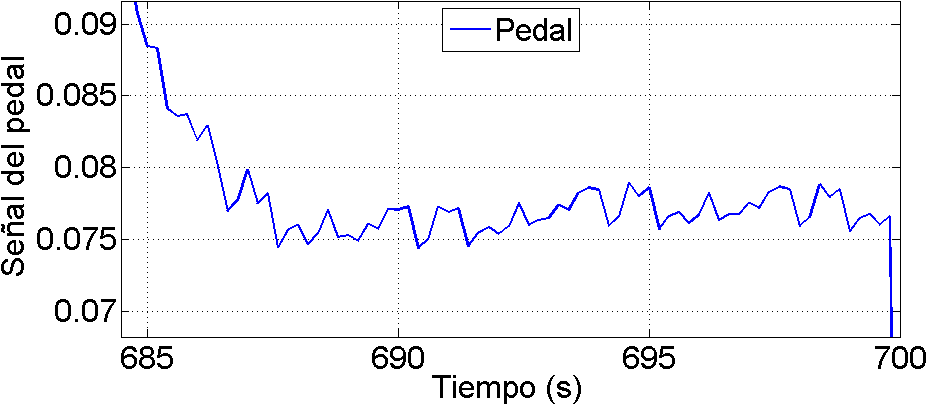
\includegraphics[width=0.5\linewidth,type=png,ext=.png,read=.png]{figures/pedalCtte}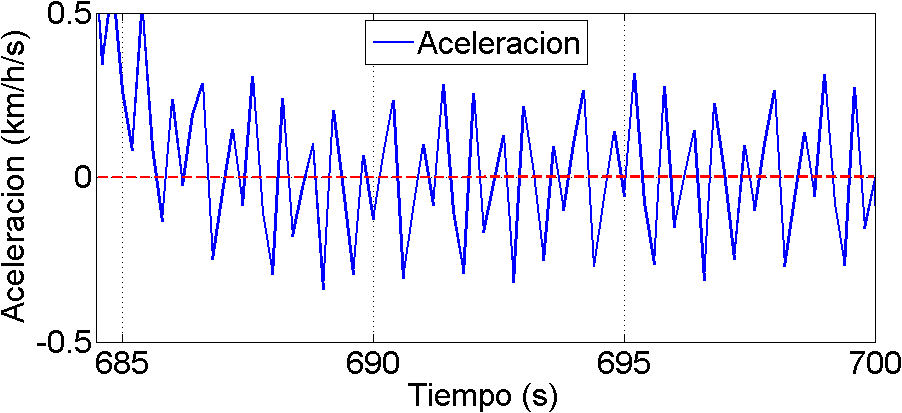
\includegraphics[width=0.5\linewidth,type=png,ext=.png,read=.png]{figures/aceCtte}
\caption{Valor del pedal (Izquierda) y aceleración del automóvil (derecha) en un tramo constante a 40 km/h.}
\label{fig:aceCtte}
\end{figure} 

Si el carro va manteniendo un velocidad constante y se genera un cambio de perfil, al comparar la aceleración actual con la óptima establecida para alcanzar la nueva velocidad, obtendremos que es necesario hacer un ajuste a los singletons, pero la mayoría de las veces el ajuste resulta ser demasiado elevado, ocasionando saltos muy grandes en la señal del pedal, y como el aumento de la aceleración negativa es más sensible a los cambios en los valores del pedal que la aceleración positiva, nos encontramos con los elevados valores en los momentos cuando se debe frenar. Para mejorar la situación, cada vez que nos encontramos con un cambio en los valores del perfil de velocidad, \textbf{dejamos que el controlador se ejecute, sin hacerle modificaciones a los singletons} durante un periodo de cinco iteraciones, de esta manera podemos probar si el controlador que se estaba utilizando para mantener la velocidad constante, se ajusta a la tarea de alcanzar la nueva velocidad.

\begin{figure}[h]
\centering
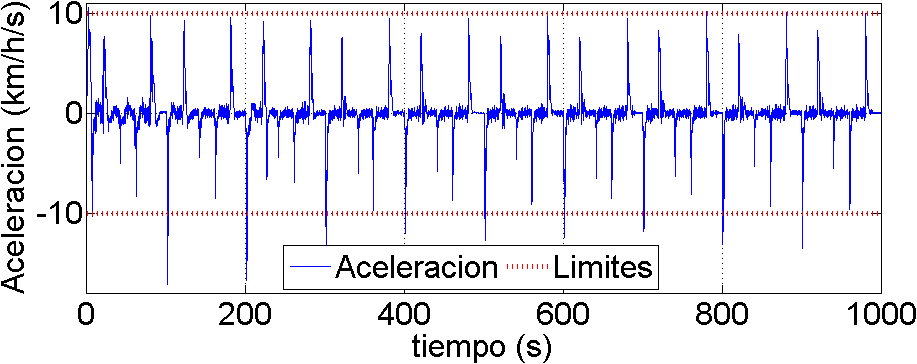
\includegraphics[width=0.6\linewidth,type=png,ext=.png,read=.png]{figures/acelFinal}
\caption{Aceleración del automóvil en un tramo constante a 40 km/h.}
\label{fig:acelFinal}
\end{figure}

Con el nuevo enfoque se logró reducir la aceleración mínima obtenida al momento de frenar de -21.80 km/h/s a -17.17 km/h/s. En la figura \ref{fig:acelFinal}, se observa que este valor se obtuvo en el primer cambio de 40 km/h a 20 km/h, y que luego de los tres primeros ciclos, al terminar los ajustes en la topología, los valores que se obtuvieron al realizar este cambio de velocidad, se encontraron entre -13 km/h/s y -11 km/h/s.
 
Con respecto a los singletons, como se muestra en la figura \ref{fig:singleFin}, se logró obtener un comportamiento muy estable. Luego de la etapa de modificación de la topología, llegó un punto en el que los singletons presentaban un comportamiento casi constante, caracterizado por pequeñas oscilaciones.


\begin{figure}[h]
\centering
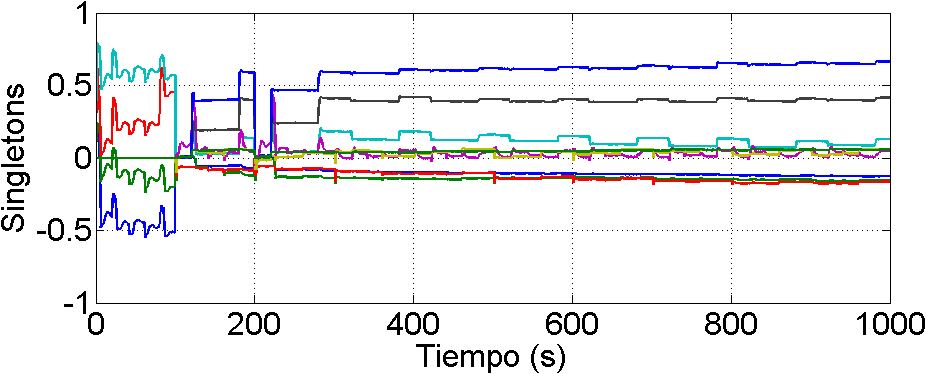
\includegraphics[width=0.6\linewidth,type=png,ext=.png,read=.png]{figures/singleFin}
\caption{Comportamiento de los singletons luego de aplicados todos los ajustes al sistema. Cada línea de color representa el valor de un singletons a lo largo de la ejecución.}
\label{fig:singleFin}
\end{figure} 


\begin{figure}[h]
\centering
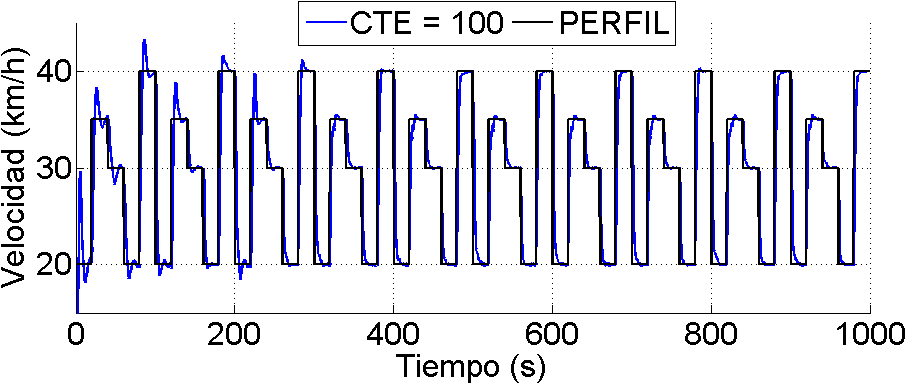
\includegraphics[width=0.6\linewidth,type=png,ext=.png,read=.png]{figures/velFin}
\caption{Velocidad del carro luego de aplicados todos los ajustes al sistema.}
\label{fig:velFin}
\end{figure} 




% Resultados1
\chapter{Pruebas} 
\label{chap:pruebas}

La fase de prueba se separó en dos partes. La primera consistió en una serie de simulaciones realizadas con TORCS (sección \ref{sec:torcs}), presentadas en la \textbf{sección \ref{sec:pTorcs}}, en la cual se utilizaron un gran número de vehículos con diferentes características y se ejecutaron la misma simulación con cada uno de ellos, de manera que se pueda comparar el desempeño del sistema entre los diferentes vehiculos. 

El segundo conjunto de pruebas se encuentran en la \textbf{sección \ref{sec:pCampo}}, consiste en la implementación del sistema en el vehículo \textbf{Platero} del grupo AUTOPIA, presentado en la sección \ref{sec:carros}. Comenzando con la \textbf{sección \ref{subsec:p15}}, donde se realizaron cinco pruebas manteniendo la velocidad del perfil constante a 15 km/h, en cada una de ellas se fue variando la configuración de los parámetros del sistema, y se compararon con una prueba donde el vehículo fue conducido manualmente por una persona. Las dos configuraciones que obtuvieron los mejores resultados se utilizaron en la \textbf{sección \ref{subsec:variandoP}}, para una prueba en la que se fue variando la consigna de velocidad. Para probar un caso extremo, en la \textbf{sección \ref{subsec:autoManual}} se realizó una comparación entre conducción manual y conducción automática a una velocidad constante a 5 km/h.  

En los gráficos de velocidad que se presentan en esta sección, se señalan los instantes donde el aprendizaje global agrega nuevas funciones de pertenencia y cuando se reducen los trapecios correspondientes a las funciones de pertenencias, utilizando los identificadores, \textbf{nuevas etiquetas} y \textbf{reducción trapecios} respectivamente.
  
\section{Pruebas realizadas con TORCS}
\label{sec:pTorcs}


Se buscó comparar el comportamiento de diferentes vehículos, que utilizaron el sistema de aprendizaje bajo las mismas condiciones. Definimos la simulación que se utilizó, con las características que se presentan en la tabla \ref{fig;sim}.

\begin{table} [htb]
\begin{minipage}{\linewidth} \centering
\begin{tabular}{|>{\columncolor[gray]{0.9}}c|c|}
\hline
 Variables de entrada & 2 \\ \hline
& Error de velocidad \\
\multirow{-2}{*}{Métricas}& Derivada del error de velocidad \\ \hline
Rango del error & [-25, 25] \\ \hline
Rango de la derivada & [-8, 8] \\ \hline
Constante de normalización & 100 \\ \hline
& 20 Km/h durante 100 iteraciones \\
& 35 Km/h durante 100 iteraciones \\ 
& 30 Km/h durante 100 iteraciones \\ 
& 20 Km/h durante 100 iteraciones \\ 
\multirow{-5}{*}{Perfil de velocidad}& 40 Km/h durante 100 iteraciones \\ \hline
Tamaño de ciclo & 500\\ \hline
Duración de la simulación & 10 ciclos \\ \hline
Pista de TORCS & longrect\footnote{Pista de TORCS en forma por dos segmentos rectos de 3 Km, unidos por en sus extremos por curvas de 100 m con angulo de 180 grados} \\ \hline
\end{tabular}
\caption{Formato de la simulación que se realizo a los diferentes tipos de carros del TORCS}
\label{fig;sim}
\end{minipage}
\end{table}

TORCS nos permite seleccionar entre un gran número de automóviles, los cuales presentan variaciones en sus atributos que lo hacen diferentes entre si. Con el propósito de probar el funcionamiento del sistema en carros con diferentes características, se realizó la misma simulación con varios de ellos.

La prueba se ejecutó con 30 automóviles distintos. Se seleccionaron siete de estos vehículos para realizar un análisis comparativo de sus atributos, el cual se presenta en la tabla \ref{tab:compCar}. Los atributos presentados en la tabla, no son lo únicos que diferencian los automóviles de TORCS, en la sección \ref{ape:atributos} del apéndice, se presentan más propiedades que pueden modificarse en los vehículos de TORCS.

\begin{table}[h] \centering
\begin{minipage}[b]{\linewidth} 
\begin{tabular}{|p{2cm}|p{2cm}|p{1cm}|p{1.1cm}|p{1cm}|c|p{1.1cm}|p{1.2cm}|}
\hline

\rowcolor[gray]{0.9} & \textbf{Modelo} & \textbf{Masa $Kg$} & \textbf{Poder $kW$} & \textbf{Cx*A\footnote{Coeficiente aerodinámico por área de incidencia del aire.} $m^2$} & \textbf{Conducción} & \textbf{Largo $m$}& \textbf{Ancho $m$} \\ \hline \hline

\parbox{2.5 cm}{\vspace{1 mm}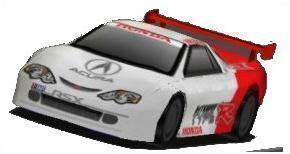
\includegraphics[scale= 0.2,type=jpg,ext=.jpg,read=.jpg]{figures/acura}\vspace{1 mm}} & Acura NSX type S-Zero & 1200 & 285 & 0.612 & Rwd\footnote{\textit{Rear Wheel Drive}, carros con tracción en las ruedas traseras.} & 5.00 & 1.92 \\ \hline

\parbox{2.5 cm}{\vspace{1 mm} 
\includegraphics[scale= 0.2,type=jpg,ext=.jpg,read=.jpg]{figures/bug}\vspace{1 mm}}&Baja Bug & 600 & 82 & 0.9 & Rwd & 3.8 & 1.8 \\ \hline

\parbox{3 cm}{\vspace{1 mm} 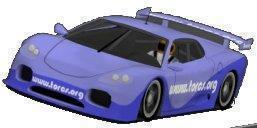
\includegraphics[scale= 0.2,type=jpg,ext=.jpg,read=.jpg]{figures/trb}\vspace{1 mm}} & Car1-trb1  & 1150 & 405 & 0.662 & Rwd & 4.52 & 1.94 \\ \hline

\parbox{2.5 cm}{\vspace{1 mm} 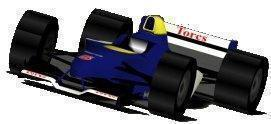
\includegraphics[scale= 0.2,type=jpg,ext=.jpg,read=.jpg]{figures/f1}\vspace{1 mm}} & sc-f1 & 650 & 677 & 0.336 & Rwd & 4.3 & 2.0 \\ \hline

\parbox{2.5 cm}{\vspace{1 mm} 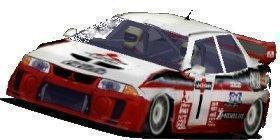
\includegraphics[scale= 0.2,type=jpg,ext=.jpg,read=.jpg]{figures/evo}\vspace{1 mm}}& Mitsubishi Lancer EVO & 900 & 321 & 0.6 & 4WD\footnote{\textit{Four Wheel Drive}, carros con tracción en las cuatro ruedas.} & 4.2 & 2.02 \\ \hline

\parbox{2.5 cm}{\vspace{1 mm} 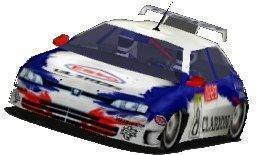
\includegraphics[scale= 0.2,type=jpg,ext=.jpg,read=.jpg]{figures/306} \vspace{1 mm}} & Peugeot 306 Maxi  & 950 & 246 & 0.77 & 4WD & 3.89 & 2.0 \\ \hline

\parbox{2.5 cm}{\vspace{1 mm} 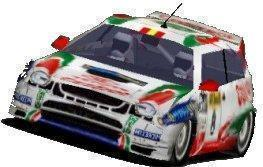
\includegraphics[scale= 0.2,type=jpg,ext=.jpg,read=.jpg]{figures/corolla}\vspace{1 mm}}& Toyota Corolla WRC  & 905 & 329 & 0.770 & 4WD & 3.81 & 1.98 \\ \hline

\end{tabular}
\caption{Tabla comparativa de los atributos de los vehículos}
\label{tab:compCar}
\end{minipage}
\end{table}

Ejecutando la simulación utilizando los siete vehículos presentados en la tabla \ref{tab:compCar}, se obtuvieron los resultados de la figura \ref{fig:7cars}. A pesar de sus diferentes dinámicas, se puede observar que el comportamiento de los siete carros es prácticamente igual, y en los casos como el que se encuentra resaltado, perteneciente a los segundos 450 y 500, los vehículos no sobrepasaron el perfil de velocidad, por mucho más de 0.5 Km/h. 

En la figura \ref{fig:31cars}, correspondiente a la simulación de los 30 carros, se observa como los grandes picos, que aparecieron en el período antes de la ejecución del aprendizaje global, disminuyeron considerablemente a medida que transcurrió la simulación. A medida que los singletons se fueron estabilizando, se fue obteniendo un mejor control y se logra disminuir la diferencia con respecto al perfil de velocidad a menos de 1 km/h, como se puede apreciar en el acercamiento realizado entre los segundos 780 y 800.   

\begin{minipage}{1\linewidth}
\end{minipage}
\begin{figure}[htb]
\centering
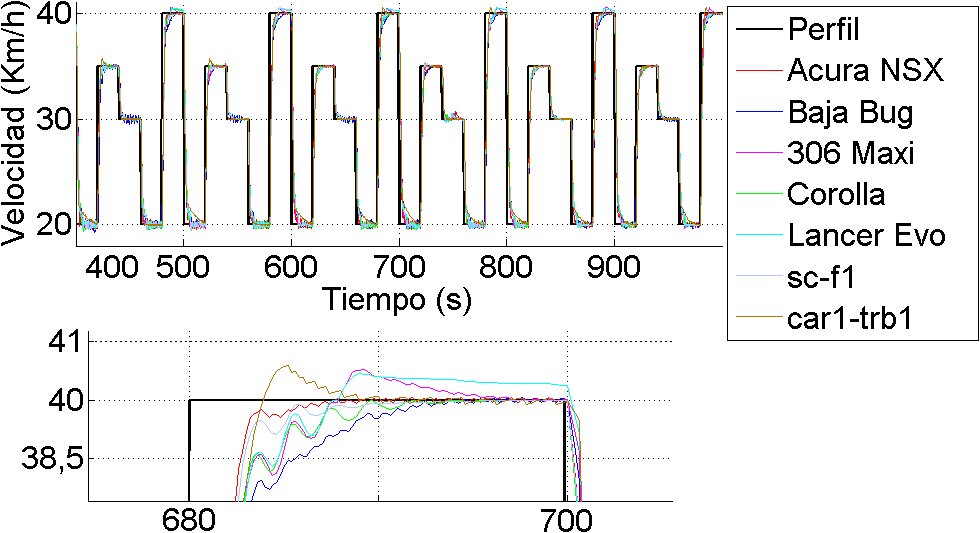
\includegraphics[width=0.6\linewidth,type=png,ext=.png,read=.png]{figures/7cars}
\caption{Velocidad de los carros entre los 400 y 1000 segundos de la ejecución de las pruebas}
\label{fig:7cars}
\end{figure}  
  
\begin{figure}[htb]
\centering
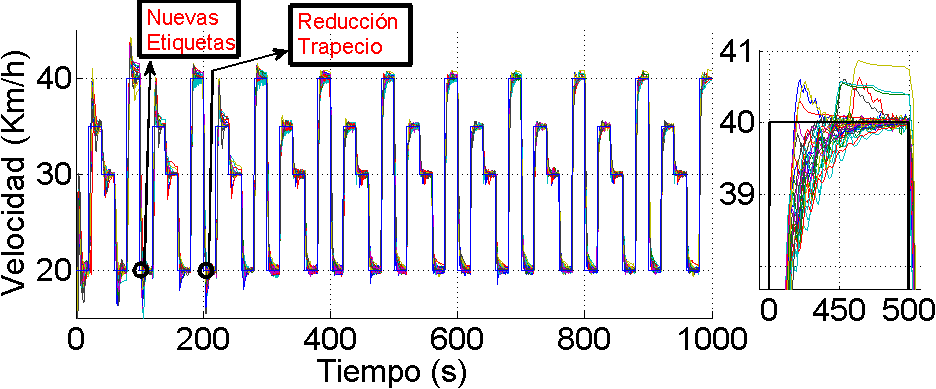
\includegraphics[width=0.6\linewidth,type=png,ext=.png,read=.png]{figures/31cars}
\caption{Velocidad de los 30 carros que corrieron la simulación.}
\label{fig:31cars}
\end{figure}


\section{Pruebas realizadas con vehículo automatizado}
\label{sec:pCampo}

Para la fase final del proyecto, se utilizó a \textbf{Platero} (sección \ref{sec:carros}) como vehículo de pruebas. Con cada prueba se buscó ajustar y mejorar el sistema, para hacerlo lo más preciso y confortable posible.

Resultados empíricos prueban que valores superiores a 0.5 sobre el acelerador producen aceleraciones muy altas sobre el vehículo, por lo que deben ser evitados con el fin de obtener un control confortable para los ocupantes del vehículo; por otra parte, valores superiores a 0.2 sobre el freno pueden producir desaceleraciones bruscas, llegando incluso a ser peligrosas \cite{Milanes2010}. Teniendo esto en cuenta, antes de comenzar con cualquier tipo de prueba, se limitó la salida correspondiente al pedal, así como los límites de los singletons, para respetar dichos valores.

Los resultados de velocidad presentados en cada experimento, se obtuvieron por medio del modulo \gls{CAN} de Platero, y poseen un error estimado de 0.1 km/h. 

\subsection{Perfil constante a 15 km/h}
\label{subsec:p15}

Para la primera prueba en Platero, se condujo el vehículo por \gls{ZOCO}, sin tener un recorrido definido, por un período de 340 segundo (1700 iteraciones), utilizando una consigna de velocidad constante a 15 Km/h. Se utilizó este valor porque es una velocidad algo complicada para el sistema, ya que la frontera del cambio automático de la transmisión entre primera y segunda es cercano a esa velocidad\footnote{No se dispone de la especificación técnica del cambio de marchas, pero se supone que dicho control no dependerá únicamente de la velocidad, lo haría también de otras variables como pueden ser las revoluciones por minuto del motor, etcétera.}, por lo que el control de velocidad se hace más inestable.

Como en los instantes iniciales de las cuatro primeras pruebas el automóvil alcanzó velocidades cercanas a los 20 km/h, se activó el cambio automático de la caja de velocidades de primera a segunda. Como parte de la prueba, se decidió en el segundo 300 (equivalente a 1500 iteraciones) reducir la velocidad de la caja de segunda a primera, manteniendola así hasta finalizar la prueba, de manera que se pudiera observar como el vehículo se adaptaba al nuevo cambio. En las dos últimas pruebas no se llegaron a  alcanzar velocidades muy por encima de 15 km/h, por lo que no se activó el cambio automático de primera a segunda, manteniendo la trasmisión en primera durante el transcurso de la prueba; se intentó la opción de hacer el cambio manual, pero el vehículo no lo permitió debido a la baja velocidad a la que circulaba. 

Para medir la eficacia del sistema, se calculó el \gls{MAE}, el cual se puede observar en la leyenda de cada figura correspondiente a la velocidad de los vehículos. En este caso como no no se realizaron variaciones en el perfil de velocidad, el \gls{MAE}, resulta un buen indicador para medir el funcionamiento del controlador.

Entre cada prueba realizada, se fueron modificando los atributos del controlador, con el fin de encontrar la configuración que otorgase el mejor desempeño. Las configuraciones utilizadas en cada prueba son presentadas en la tabla \ref{tab:compCar}.

\begin{table}[!h]
\centering
\begin{tabular}{|c|c|c|c|}
\hline 
\rowcolor[gray]{0.9} Prueba &  $Cte$ & Rango & Etiquetas\\
\hline \hline 
0  & 100 & \parbox[t]{3cm} {\hspace{8 px} $\varepsilon=[-20,20]$ \\ $\frac{d(\varepsilon)}{d(t)}=[-8,8]$ \vspace{1mm}} &  \parbox[t]{3cm} {\hspace{11 px}$\varepsilon=2$\\ $\frac{d(\varepsilon)}{d(t)}=2$} \\ 
\hline 

1 & 100 & \parbox[t]{3cm} {\hspace{8 px} $\varepsilon=[-20,20]$ \\ $\frac{d(\varepsilon)}{d(t)}=[-5,5]$} &  \parbox[t]{3cm} {\hspace{11 px}$\varepsilon=2$\\ $\frac{d(\varepsilon)}{d(t)}=2$} \\ 
\hline 

2 & 200 & \parbox[t]{3cm} {\hspace{8 px} $\varepsilon=[-20,20]$ \\ $\frac{d(\varepsilon)}{d(t)}=[-5,5]$} &  \parbox[t]{3cm} {\hspace{11 px}$\varepsilon=2$\\ $\frac{d(\varepsilon)}{d(t)}=2$} \\ 
\hline 

3 & 100 & \parbox[t]{3cm} {\hspace{8 px} $\varepsilon=[-10,10]$ \\ $\frac{d(\varepsilon)}{d(t)}=[-5,5]$} &  \parbox[t]{3cm} {\hspace{11 px}$\varepsilon=2$\\ $\frac{d(\varepsilon)}{d(t)}=2$} \\ 
\hline 

4 & 100 & \parbox[t]{3cm} {\hspace{8 px} $\varepsilon=[-20,20]$ \\ $\frac{d(\varepsilon)}{d(t)}=[-5,5]$} &  \parbox[t]{3cm} {\hspace{11 px}$\varepsilon=4$\\ $\frac{d(\varepsilon)}{d(t)}=2$} \\ 
\hline

5 & 100 & \parbox[t]{3cm} {\hspace{8 px} $\varepsilon=[-20,20]$ \\ $\frac{d(\varepsilon)}{d(t)}=[-5,5]$ \\ $perfil=[0,40]$} &  \parbox[t]{3cm} {\hspace{11 px}$\varepsilon=4$\\ $\frac{d(\varepsilon)}{d(t)}=2$\\$perfil=2$} \\ 
\hline  
\end{tabular}
\caption{Comparación entre los parámetros de las pruebas realizadas con un perfil de velocidad constante a 15 km/h}
\label{tab:comparacionPruebas}
\end{table}



\begin{figure}[h]
\centering
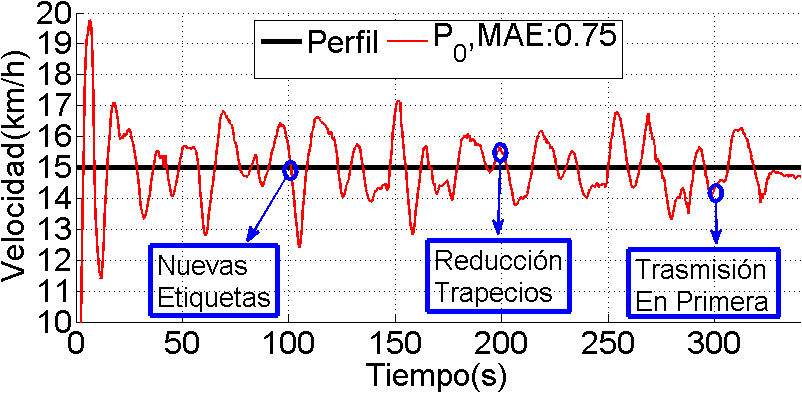
\includegraphics[width=0.45\linewidth]{figures/p0.png}\hspace{0.5cm}
\includegraphics[width=0.45\linewidth]{figures/p1.png}\\
\includegraphics[width=0.45\linewidth]{figures/p2.png}\hspace{0.5cm}
\includegraphics[width=0.45\linewidth]{figures/p3.png}\\
\includegraphics[width=0.45\linewidth]{figures/p5.png}\hspace{0.5cm}
\includegraphics[width=0.45\linewidth]{figures/final15.png}
\caption{Velocidad del vehículo durante las pruebas a 15 km/h. Prueba 0 (arriba izquierda), Prueba 1 (arriba derecha), Prueba 2 (centro izquierda), Prueba 3 (centro derecha), Prueba 4 (abajo izquierda) y Prueba 5 (abajo derecha)}
\label{fig:pruebas15}
\end{figure}


En la figura \ref{fig:pruebas15}, se muestran los resultados obetidos en las cinco pruebas realizadas a 15 km/h. La \textbf{prueba 0} (figura \ref{fig:pruebas15} arriba izquierda) se realizó para comprobar que el sistema funcionara correctamente al ser adaptado al programa de control del vehículo. La configuración utilizada durante la ejecución no varió mucho de la utilizada con \gls{TORCS}, solo se redujo el rango del error a [-20,20]. No ocurrió ningún percance durante la ejecución de la prueba. Exceptuando los primero instantes cuando tiene que pasar de 0 km/h a 15 km/h, la diferencia entre la velocidad del automóvil y el perfil de velocidad, no llega a ser superior a los 3 km/h. 

En la \textbf{prueba 1} (figura \ref{fig:pruebas15} arriba derecha) se observa una pequeña mejora con respecto a la \textit{prueba 0}, debido a que se redujo el rango de la derivada del error de velocidad a [-5,5], con lo que se logró disminuir el \gls{MAE} a 0.64, y se redujeron un poco el tamaño de las oscilaciones.

Se aumentó la constante de normalización de 100 a 200 en la \textbf{prueba 2} (figura \ref{fig:pruebas15} centro izquierda), para intentar disminuir la magnitud de los cambios de los singletons, y buscar disminuir las oscilaciones con respecto al perfil de velocidad. Con esta configuración se obtuvieron los peores resultados, las oscilaciones fueron muy grandes, y se alcanzaron diferencias con respecto a la velocidad deseada superiores a 2 km/h. Se obtuvo un \gls{MAE} de 1.1, el cual fue el más elevado que se obtuvo entre todas las pruebas.

Tomando en cuenta los malos resultados de la \textit{prueba 2}, se retomó la constante de normalización con un valor de 100 para la \textbf{prueba 3} (figura \ref{fig:pruebas15} centro derecha). Aunque obtuvo un \gls{MAE} de 0.64, al igual que la \textit{prueba 1}, se observa que a partir del segundo 200, la velocidad del vehículo logró estabilizarse un poco, reduciendo el tamaño de las oscilaciones. En la \textit{prueba 1}, las oscilaciones solo parecen reducirse, en el segundo 300, cuando se bajó la caja de cambio de segunda a primera.    

En estas cuatro primeras pruebas, al realizar el cambio en la transmisión velocidad de segunda a primera, resulto más fácil para el vehículo mantener una velocidad cercana a los 15 km/h, logrando que las oscilaciones disminuyeran considerablemente.

La primera prueba que no realizó el gran salto en velocidad que presentaron las anteriores al pasar de 0 km/h a 15 km/h fue la \textbf{prueba 4} (figura \ref{fig:pruebas15} abajo izquierda), esto se debe a que se utilizaron cuatro etiquetas para el error de velocidad en vez de dos. Esta configuración obtuvo los mejores resultados, logrando el mínimo \gls{MAE}. La única oscilación grande que se puede apreciar, se encuentra luego del segundo 100, que es el instante cuando se ejecuta el aprendizaje global y se reinician los singletons; pero luego al estabilizarse, la diferencia entre la velocidad del perfil y la velocidad del carro, ni siquiera llega a ser 1 km/h. Esta y la siguiente prueba se realizaron con la transmisión en primera velocidad durante toda la ejecución, ya que el controlador nunca revolucionó lo suficiente como para permitir hacer el cambio manual.

En la \textbf{prueba 5} (figura \ref{fig:pruebas15} arriba derecha) \textbf{se agregó el valor del perfil de velocidad como tercera variable de entrada}, con la finalidad de lograr un mejor control al momento de mantener la velocidad constante. Desde el punto de vista del pedal, no implica lo mismo mantener al vehículo constante a una velocidad u otra, la variable de entrada adicional permite marcar esta diferencia y controlar mejor cada caso que pueda presentarse. Aunque los resultados fueron muy buenos, no llegaron a ser mejores que los de la \textit{prueba 4}, ya que obtuvo un \gls{MAE} un poco mayor.

 
\subsubsection*{Comparación entre conducción automática y conductor humano}
\label{subsec:autoManual}

Para comparar el desempeño del sistema con la manera de manejar de un persona, se hizo una prueba en la que no se activó el control de conducción automática, sino que se manejó manualmente durante el mismo periodo de tiempo que duraron las pruebas, intentando mantener la velocidad constante a 15 km/h.    

\begin{figure}[!h]
\centering
\includegraphics[width=0.6\linewidth]{figures/manual.png}
\caption{Velocidad del automóvil conducido de forma manual.}
\label{fig:manual}
\end{figure}

Como se observa en la figura \ref{fig:manual} se obtuvieron mejores resultados utilizando la configuración de la \textit{prueba 4}, que la persona que condujo el carro durante la prueba manual, lo cual se ve reflejado en el \gls{MAE}; en la prueba manual fue de 0.46, y en la \textit{prueba 4} fue de 0.39. Se debe tener en cuenta que la reinicialización de los singletons contribuyeron al aumento del \gls{MAE} en las pruebas, porque en ese instante ocurrió una reducción muy significativa de la velocidad, debido a que el vehículo comenzó desde cero el proceso de aprendizaje.

\subsection{Variando el perfil a lo largo de la ejecución}
\label{subsec:variandoP}

Debido a los buenos resultados obtenidos con la configuración de la \textit{prueba 4}, se seleccionó dicho modelo para realizar una prueba en la cual vamos a ir variando el perfil de velocidad. De esta manera se  analizó la forma en que se adaptó el aprendizaje del controlador a los constantes cambios en la consigna de velocidad.

\begin{figure}[htb]
\centering
\includegraphics[width=0.6\linewidth, height = 3cm]{figures/zoconp6.png}
\caption{Recorrido utilizado para la prueba con variación en el perfil de velocidad.}
\label{fig:zoconp6}
\end{figure}

La prueba se realizó circulando por el recorrido que se muestra en la figura \ref{fig:zoconp6}, partiendo del punto \textit{A}. Los cambios en el perfil se van a realizar en los puntos marcados en el mapa de la pista, el tramo entre el punto \textbf{B} y el punto \textbf{C} consiste en una pendiente que presenta un desnivel de aproximadamente 2\%, mientras que el resto de la pista no presenta mayores diferencias de elevación. Debido al reducido tamaño de la pista, la velocidad máxima a la que se llegó el vehículo fue 40 km/h.

En la figura \ref{fig:pPerfil} se puede observar la velocidad del controlador con respecto al perfil de velocidad que se utilizó a lo largo de la prueba. A simple vista se observa que el sistema tuvo un desempeño muy bueno, no se observan diferencias muy grandes con respecto al perfil. La figura \ref{fig:v1} se ve con detalle los resultados correspondientes a la velocidad y se especifica los puntos de la pista por los que pasaba el vehículo.

%\begin{figure}[htb]
%\centering
%\includegraphics[width=0.6\linewidth]{figures/p6.png}
%\caption{Velocidad del vehículo durante la prueba con variación en el perfil de velocidad.}
%\label{fig:pPerfil}
%\end{figure}

Durante la primera vuelta no se modificó el perfil hasta que se llegó al punto \textbf{C} como puede apreciarse en la figura \ref{fig:v1} (arriba), ya que se utilizó el tramo \textbf{A-C} para que el controlador se adaptase lo mejor posible antes de realizar el primer cambio.

\begin{figure}[htb]
\centering
\includegraphics[width=0.65\linewidth]{figures/p61.png}
\includegraphics[width=0.65\linewidth] {figures/p62.png}
\caption{Velocidad del vehículo indicando los puntos de la pista por los que pasa el vehículo, durante la prueba con variación en el perfil de velocidad. Primera mitad (izquierda), segunda mitad (derecha).}
\label{fig:v1}
\end{figure}

Desde el comienzo de la prueba hasta que llegamos al punto \textbf{D}, no se observa una diferencia muy grande entre la velocidad deseada y la velocidad real del vehículo; a diferencia del tramo siguiente, en el que luego del segundo 100, nos encontramos con diferencias de hasta 3 km/h. La variación en la velocidad, se debe a que en ese instante de tiempo se activó el aprendizaje global y se reiniciaron los singletons del controlador. En la segunda mitad de la prueba (figura \ref{fig:v1} abajo), el vehículo se comportó de manera excepcional, ajustándose a los cambios de velocidad sin ningún problema.

\definecolor{bb}{RGB}{99,184,255}
\begin{table}[htb]
\centering
\begin{minipage}{\linewidth}
\begin{tabular}{|c|c|c|c|c|c|}
\hline 
\rowcolor[gray]{0.9} \parbox[t]{2cm}{\textbf{Tramo km/h}}& \parbox[t]{2cm}{\textbf{Aceleración\\Media km/h/s}\vspace{1mm}} & \parbox[t]{2cm}{\textbf{Aceleración \\en $V_p$ $\pm 0.5$ km/h/s}} & \parbox[t]{2cm}{\textbf{Error\\ Medio km/h}} & \parbox[t]{2cm}{\textbf{Error\\ Máximo km/h}} & \parbox[t]{2cm}{\textbf{Error\\ Mínimo km/h}} \\ 
\hline \hline 
0-15 & 6.82 & 8.67 & 0.36 & 1.08 & -1.01 \\ 
\hline 
15-25 & 6.25 & 4.66 & 0.66 & 1.53 & -1.05 \\ 
\hline 
25-15 & \cellcolor{bb}  -5.56 & -4.79 & 1.39 & 3.27 & -3.56 \\ 
\hline 
15-30 & 3.26 & 2.61 & 0.42 & 0.79 & -1.09 \\ 
\hline 
30-15 & \cellcolor{bb} -6.25 & -7.38 & 0.48 & 0.72 & -1.09 \\ 
\hline 
15-20 & *\footnote{La aceleración media se midió hasta que se alcanza la velocidad de la consigna más o menos 5 km/h, por lo que no se pudo calcular en este caso.} & 0.61 & 0.36 & 0.68 & -0.70 \\ 
\hline 
20-10 &\cellcolor{bb} -6.25 & -5.12 & 0.29 & 0.55 & -1.12 \\ 
\hline 
10-35 & 4.63 & 2.81 & 0.37 & 0.79 & -0.71 \\ 
\hline 
35-15 &\cellcolor{bb} -7.14 & -8.42 & 0.52 & 0.56 & -1.18 \\ 
\hline 
15-40 & 4.03 & 2.09 & 0.79 & 1.40 & -0.80 \\ 
\hline 
40-10 &\cellcolor{bb} -6.82 & -7.85 & 0.24 & 0.75 & -0.41 \\ 
\hline 
10-25 & 5.77 & 4.26 & 0.32 & 0.67 & -0.67 \\ 
\hline
25-10 &\cellcolor{bb} -8.33 & -9.21 & 0.30 & 0.76 & -0.85 \\ 
\hline
10-30 & 4.55 & 1.81 & 0.34 & 0.60 & -0.68 \\ 
\hline
30-15 &\cellcolor{bb} -8.33 & -8.85 & 0.36 & 0.66 & -0.36 \\ 
\hline
15-40 & 5.43 & 4.34 & 0.37 & 0.46 & -0.86 \\ 
\hline
40-10 &\cellcolor{bb} -7.50 & -5.62 & 0.29 & 0.94 & -0.79 \\ 
\hline
10-20 & 6.25 & 3.70 & 0.57 & 1.07 & -1.14 \\ 
\hline
20-5 &\cellcolor{bb} -7.50 & -8.84 & 0.36 & 1.11 & -0.70 \\ 
\hline
\end{tabular}
\end{minipage} 
\caption{Valores correspondientes a los tramos de cambio de velocidad}
\label{tab:p6}
\end{table}

En la tabla \ref{tab:p6} se presentan valores correspondientes a la aceleración y velocidad obtenidos durante la prueba. \textbf{La aceleración media} se midió desde el momento en que ocurre un cambio de perfil, hasta que se alcanza la velocidad del perfil más o menos 5 km/h; \textbf{la aceleración en $V_p\pm0.5$} corresponde a la aceleración cuando se reduce a $\pm0.5$ km/h el error de velocidad entre el vehículo y el perfil, justo después de ocurrir un cambio en la consigna. 

Los valores que están resaltados en azul en la tabla \ref{tab:p6}, corresponden a la aceleración media en los tramos donde el carro se encontraba frenando, dichos valores presentan tendencia hacia los -8km/h/s, por lo que se puede decir que la aceleración media cuando el vehículo desacelera es aproximadamente igual a la aceleración de confort; en cambio cuando el automóvil acelera, la aceleración media tiende a 4 km/h/s, lo que es equivalente a la mitad de la aceleración de confort. La discrepancia en la tendencia de la aceleración media en ambos casos, indica que el efecto del pedal de freno sobre el estado del vehículo influye de mayor manera que el pedal del acelerador.  

\textbf{El error medio, error máximo y error mínimo}, se calcularon a partir del punto en que se alcanza $V_p\pm0.5$, hasta que ocurrió un cambio en el perfil de velocidad. Únicamente en el tercer tramo, el cual va de 25 a 15 km/h, el error medio fue mayor a 1 km/h; esto gracias a que en este tramo se insertaron nuevas etiquetas a las variables de entrada y se reinicializaron los singletons. En general los errores máximos y mínimos son muy bajos, encontrándose la mayoría al rededor de $\pm 1$ km/h.

Teniendo en cuenta que los velocímetros analógicos, tienen una precisión de 10 km/h, y tanto estos como los digitales  no son completamente exactos,  podemos decir que los valores obtenidos en esta prueba son muy favorables, y la diferencias de velocidad entre el vehículo y el perfil, resulta casi imperceptible para el conductor. 
\begin{figure}[htb]
\centering
\includegraphics[width=0.6\linewidth]{figures/finalcambios.png}
\caption{Resultado de prueba cambiando el perfil de velocidad, utilizando controlador con tres variables de entrada}
\label{fig:finalcambios}
\end{figure}

\begin{table}[htb]
\centering
\begin{tabular}{|c|c|c|c|}
\hline 
\rowcolor[gray]{0.9} \textbf{Configuración} & \parbox[t]{3.5cm}{\textbf{Media del error medio km/h}} & \parbox[t]{3.5cm}{\textbf{Media del error máximo km/h}} & \parbox[t]{3.5cm}{\textbf{Media del error mínimo km/h}} \\ 
\hline \hline 
\parbox[t]{3.5cm}{Prueba 4 (dos variables entradas)}& 0.36 & 1.11 & -0.70 \\ \hline
\parbox[t]{3.5cm}{Prueba 5 (tres variables entradas)} & 0.39 & 1.67 & -1.45 \\ \hline
\end{tabular}
\caption{Tabla comparativa de las medias de los errores entre configuración con dos variables de entrada y tres variables de entrada.}
\label{tab:medias}
\end{table}

En el tabla \ref{tab:medias}, se comparan las medias de los errores, medio, máximo y mínimo, correspondientes a la configuración de tres variables de entrada, con las medias de los resultados obtenidos utilizando la configuración de 2 variables de entrada, que se presentan en la tabla \ref{tab:p6}. Como se puede observar, la diferencia de la media del error medio entre los dos es muy pequeña, pero la diferencia entre los errores mínimos y máximos de cada uno es notable; con la media del error mínimo de la configuración de tres variables de entrada llegando a ser el doble de la de dos variables, lo que indica que aunque la diferencia no es mucha, no hay mejora utilizando tres variables de entrada.  

\subsection{Comparación entre conducción automática y conducto humano a una velocidad constante de 5 km/h}

%Comparación entre conducción automática y conducción manual realizada por una persona a una velocidad constante de 5 km/h

Para probar que tan preciso puede llegar a ser el sistema en un caso extremo, se realizó una nueva comparación entre la capacidad de una persona contra la del sistema de mantener la velocidad del vehículo constante, pero a una velocidad de a 5 km/h. Se eligió un valor muy pequeño, porque a esa velocidad los efectos del pedal y las diferencias de elevación de la pista, por muy pequeñas que sean, causan un mayor impacto en la aceleración del vehículo; de manera tal, que mantener la velocidad casi constante, se convierta en una tarea muy complicada. Se configuró el sistema de la misma manera que en la \textit{prueba 4} de la sección \ref{subsec:p15}, ya que fue la que obtuvo los mejores resultados.

\begin{figure}[htb]
\centering
\includegraphics[width=0.6\linewidth]{figures/AutoVsManual.png}
\caption{Comparación entre un vehículo conducido de forma manual, contra uno con conducción automática, ambos a una velocidad constante a 5 km/h.}
\label{fig:autoVsmanual}
\end{figure}

Como se puede ver en la figura \ref{fig:autoVsmanual}, el sistema de conducción automática obtuvo mejores resultados que el conductor humano. Aunque casi llega al doble de la velocidad esperada en los primeros instantes, el sistema obtuvo un \gls{MAE} mucho menor al de la persona.

En el segundo 150 de la prueba, se puede observar que el sistema casi llega a los 7 km/h, esto se debe a que el aprendizaje global se ejecutó justo un poco antes de comenzar la pendiente en bajada, por lo que el controlador tardó un poco más de tiempo en estabilizarse, luego de eso el controlador logra mantenerse muy cerca de la velocidad deseada, lo cual ocurre al empezar a subir por la pendiente de la pista. Durante el transcurso de la prueba, el velocímetro digital que posee el vehículo, se mantuvo en cero, y solo algunas veces, indicaba que íbamos a una velocidad de 5 o 6 km/h.   
% Resultados1
\chapter{Adaptación al control automático del volante} 
\label{chap:volante}

Dado que el sistema se diseñó de la manera más mas genérica posible, se decidió probar el funcionamiento del mismo en el control del volante. El proceso de adaptación consistió en: Ajustar el valor de las variables de entrada que utiliza el sistema, obviar las condiciones correspondientes al cambio de pedal, realizar el cálculo de las variables de entradas asociadas al control del volante y hacer que la modificación de los singletons fuera \textit{simétrica}, ya que las mismas acciones para girar el volante si vamos a agarrar una curva hacia la izquierda, deben ser iguales a las aplicadas para agarrar una curva hacia la derecha, pero con signo contrario.

Utilizamos dos variables de entrada en el controlador, la desviación lateral medida en metros y la variación de la desviación lateral (m/s). En \gls{TORCS} la desviación lateral se calcula con respecto al medio de la pista, en Platero es con respecto a un mapa predefinido, el cual se carga al activar el programa de control automatizado. Ambas variables de entrada fueron limitadas en el rango [-3,3] y fueron inicializadas con 3 etiquetas. Utilizamos 1 m/s como valor de aceleración de confort y una constante de normalización de 100 que fue la misma utilizada para el control del pedal. 

Para el control de los pedales, se había establecido que para representar el cambio de un pedal a otro, se devolvía cero durante tres ejecuciones del sistema; y para evitar ciertos cambios de pedal innecesario, para cada salida cuyo valor absoluto sea menor a 0.02 se devolvía cero. Estos dos casos fueron obviados cuando se establece que el sistema se va a encargar del control del volante.

\section{Pruebas realizadas con TORCS}

Para comprobar el funcionamiento del sistema al hacerse cargo del control del volante, se realizaron pruebas en \gls{TORCS} utilizando la pista \textit{Alpine-1}. Como se puede ver en la figura \ref{fig:alpine} (izquierda), el recorrido realizado, que va desde el punto \textbf{A} hasta el punto \textbf{B}, posee una gran cantidad de curvas, siendo muchas de ellas muy cerradas, lo cual representa una muy buena prueba para demostrar el funcionamiento del sistema. La prueba se realizó dejando al sistema controlar simultáneamente los pedales y el volante, la velocidad del automóvil se colocó a 15 km/h, ya que por cuestiones de seguridad las pruebas con Platero se iban a realizar a una velocidad muy baja, de modo que se hizo la prueba lo más parecida posible a lo que se tenía pensado hacer con Platero.  

\begin{figure}[htb]
\centering
\includegraphics[width=0.2\linewidth]{figures/alpine.PNG}\hspace{0.02\linewidth}\includegraphics[width=0.6\linewidth]{figures/desvTorcs.png}
\caption{Pista Alpine-1 de TORCS (izquierda). Desviación lateral con respecto al tiempo (derecha).}
\label{fig:alpine}
\end{figure}

Como se puede ver en la figura \ref{fig:alpine} (derecha), que representa la desviación del vehículo con respecto del medio de la pista, se obtuvieron muy buenos resultados. En la primera curva es donde ocurre la mayor diferencia y esto se debe a que en ese instante, los singletons se encontraban todos en cero. Luego de la segunda gran curva, un poco antes del segundo 500, el sistema logró mantener la desviación en el rango [-1,1], hasta que un poco después del instante 1000, toma la última gran curva llegando a una desviación de 1.5, para luego estabilizarse nuevamente y mantener una desviación muy baja.


\section{Pruebas realizadas con vehículo automatizado} 

Utilizando Platero cargamos un mapa que consistió en una vuelta alrededor de \gls{ZOCO}, como se puede apreciar en la figura \ref{fig:zocoV}, y con la misma configuración que se utilizó en la simulación con \gls{TORCS}, se procedió a realizar las pruebas. Por cuestiones de seguridad, el control de los pedales se dejó manual, y se condujo el vehículo a una velocidad aproximada de 10 Km/h; con respecto a la salida del volante, para evitar cambios muy bruscos, se restringió que entre dos salidas consecutivas del controlador la diferencia entre ellas no podía ser mayor a 50 grados.

\begin{figure}[htb]
\centering
\includegraphics[width=0.48\linewidth]{figures/vuelta1.png}\hspace{0.04\linewidth}\includegraphics[width=0.48\linewidth]{figures/vuelta2.png}
\includegraphics[width=0.5\linewidth]{figures/vuelta3.png}
\caption{Trayectoria del vehículo durante las tres vueltas que se realizaron.}
\label{fig:zocoV}
\end{figure}  

En la figura \ref{fig:desvPlatero} se puede observar como el sistema a medida que fue aprendiendo fue reduciendo la desviación lateral considerablemente, especialmente cuando debía pasar por la primera gran curva, que como se puede ver en la figura \ref{fig:zocoV}, cada vez se tomaba mejor, pasando de una desviación lateral de -5.37 obtenida en la primera vuelta a -2.46 que se obtuvo en la tercera vuelta.   

\begin{figure}[htb]
\centering
\includegraphics[width=0.8\linewidth]{figures/desviacionPlatero.png}
\caption{Desviación lateral entre el vehículo y el mapa.}
\label{fig:desvPlatero}
\end{figure}

Uno de los inconvenientes que se encontró, fue que como los mapas que se cargaban en Platero para especificar la ruta debían ser construidos a mano especificando las coordenadas de diversos puntos del mapa por los que el vehículo debe pasar, cada vez que se pasaba por uno de esos puntos, el automóvil cambiaba la referencia con respecto a la línea con la cual se calculaba la desviación lateral. Al obtener la desviación con respecto a la nueva referencia, en la mayoría de los casos resultaba que la desviación era muy grande, por lo que obtuvimos ciertos momentos en la prueba donde el volante hacía un movimiento brusco para poder ajustarse a la nueva línea de referencia.
% Conclusiones
\chapter{Conclusiones y recomendaciones} 

\glsreset{ITS}

La conducción automática de vehículos es un problema de gran complejidad, ya que no solo hay que considerar la dinámica y condiciones del vehículo, sino que la operación del sistema depende de la interacción entre el automóvil y el ambiente. Con los \gls{ITS} se busca mejorar la seguridad y movilidad de la red de transporte, de manera que los usuarios puedan disfrutar de beneficios  como la reducción del tráfico, tiempo de viaje, consumo de combustible, etc.

En este trabajo se ha presentado la implementación exitosa de un sistema de aprendizaje de controladores difusos para la conducción autónoma de vehículos, caracterizado por ser un sistema de aprendizaje on-line, con un tiempo de respuesta muy pequeño y la capacidad de modificar la estructura del controlador; tanto el consecuente de las reglas utilizadas, por medio del aprendizaje local, como la topología del controlador, por medio del aprendizaje global. Con especificar el número de variables de entradas, los rangos y número de funciones de pertenencia de cada variable, el sistema se encarga de realizar el ajuste a los singletons correspondientes a cada regla, los cuales pueden comenzar inicializados en cero o con una configuración previamente establecida.

El sistema se ha probado en un entorno simulado, obteniendo muy buenos resultados en los 30 automóviles con los que se realizaron las pruebas, exponiendo su poder de adaptarse a las diferentes dinámicas de cada vehículo. Se ajusta a los cambios de velocidad de muy buena manera, manteniendo la aceleración del vehículo en un rango establecido entre [-10,10] Km/h/s y desacelerando conforme el error de velocidad se acerca a cero, para luego lograr mantener el error velocidad en un rango entre [-1,1] Km/h.

Se realizaron varias pruebas utilizando un vehículo automatizado, demostrando que puede adaptarse a la dinámica, condiciones  y controles de un vehículo real. Gracias a un análisis exhaustivo, se consiguió una configuración para el sistema, la cual ha obtenido resultados excepcionales, logrando conducir mejor que una persona, ya que durante el transcurso de las pruebas comparativas que se realizaron entre los dos, el sistema pudo mantener el error de velocidad en un valor más cercano a cero que el logrado por el conductor humano. 

El sistema fue probado en el control automático del volante, donde obtuvo buenos resultado, logrando mantener la desviación lateral en un rango aceptable, y demostró la capacidad que posee de ser adaptado para la automatización de diversos controles, con solo realizar unos pequeños ajustes al código.

Con respecto a trabajos a futuros, se recomienda realizar una mejora a la etapa de aprendizaje global, particularmente a la hora de agregar nuevas etiquetas a las variables de entrada, ya que al finalizar este proceso, se reinicializan los singletons del controlador, lo que implica perder todo el aprendizaje que se había adquirido hasta ese instante. Acerca del control del volante, se deben realizar más pruebas para poder encontrar la mejor configuración posible y ajustar los valores para que se pueda lograr un mejor desempeño. 

El sistema se diseñó lo más genérico posible teniendo en mente futuras aplicaciones, en especial, realizar maniobras en conjunto con otros vehículos, como control de crucero entre dos automóviles; lo cual consiste en tener dos vehículos circulando, y cuando uno se encuentra con el otro, este debe tomar en cuenta la velocidad del otro y adaptarse a dicha velocidad y mantener una distancia prudente con el otro automóvil.
% Establece las citas y bibliografia
\bibliographystyle{plain}
\bibliography{myrefs}
% Crea el apendice
\appendix
\chapter{CSIC}
\label{ape:csic}


El Grupo ha contado con la financiación proveniente de diversos proyectos de investigación, en la sección \ref{ape:csic}, entre los que cabe destacar:

\begin{itemize}
	
	\item \textbf{\gls{ORBEX}}. Financiado por la CICYT, se definió e implementó el núcleo de un sistema de inferencia difusa, el cual se emplea en la actualidad para dar soporte a los diferentes sistemas de navegación de los vehículos. La estructura del sistema se definirá en detalle en la sección \ref{sec:orbex}.
	
	\item \textbf{\gls{ZOCO}}. Igualmente financiado por la CICYT y que permitió la construcción de la pista de experimentación en la cual se llevan a cabo las pruebas del presente trabajo. También se detallarán los aspectos de la pista de pruebas en la sección \ref{sec:zoco}.
	
	\item \textbf{COVAN} y \textbf{GLOBO}, financiados respectivamente por la Comunidad Autónoma de Madrid y la CICYT, sirvieron para comprar e instrumentar dos fugonetas \textit{Citroën Berlingo} eléctricas con las que se llevaron a cabo los primeros experimentos de conducción autónoma \cite{Alcalde2000}.
	
	\item \textbf{ISAAC} e \textbf{ISAAC-2}, financiados ambos por el extinto Ministerio de Ciencia y Tecnología, donde en colaboración con grupos de la Universidad de Alcalá de Henares, la Universidad Politécnica de Madrid y la Universidad de Extremadura, se desarrollaron sistemas para reconocer el entorno de los vehículos mediante diferentes técnicas.
	
	\item \textbf{CYBERCARS-2} fue un proyecto financiado por la Comunidad Europea, trataba sobre la realización de maniobras cooperativas entre vehículos de diferente naturaleza y en él participaron hasta once instituciones del sector del transporte.
	
	\item \textbf{MARTA} y \textbf{GUIADE} fueron financiados por el Ministerio de Fomento y están en desarrollo; buscan encontrar aplicaciones reales en automoción junto a grandes empresas españolas del sector.
	
	\item \textbf{CITYELEC} es un proyecto singular concedido a finales de 2009 y que, en una línea solidaria con el medio ambiente, busca la implementación en ciudades españolas de un flujo de tráfico verde.
	
\end{itemize}
% Apendice
\chapter{ORBEX}

En la sección \ref{ape:diseno} se explica como diseñar un controlador utilizando ORBEX, en la sección \ref{ape:gramatica} se indica la gramática para generar reglase y en la sección \ref{ape:orbex} presenta un ejemplo de un controlador definido en ORBEX. 

\section{Diseño de controlador}
\label{ape:diseno}

Para el diseño de un controlador con \gls{ORBEX} es necesario especificar 3 secciones fundamentales:
\begin{itemize}
    
    \item Las variables de entrada al sistema con sus respectivas particiones difusas o etiquetas lingüísticas. Esta sección se inicia con la cadena \textit{Entradas:}, seguida de las definiciones de las variables de entrada. La definición de variables de entrada se hará siguiendo el siguiente formato, donde \textit{(A,B,C,D)} define una función de pertenencia
    trapezoidal:\\\texttt{Entrada$_{1}$   \{Etiqueta$_{11}$ A$_{11}$ B$_{11}$ C$_{11}$ D$_{11}$ \\Etiqueta$_{12}$ A$_{12}$ B$_{12}$ C$_{12}$ D$_{12}$}
    ...\}\\\texttt{Entrada$_{2}$   \{Etiqueta$_{21}$ A$_{21}$ B$_{21}$ C$_{21}$ D$_{21}$ \\Etiqueta$_{22}$ A$_{22}$ B$_{22}$ C$_{22}$ D$_{22}$}
    ...\}
    
    \item Las variables de salida del sistema con sus respectivas particiones (singleton). Esta sección se inicia con la cadena \textit{Salidas:}, seguida de las definiciones de las variables de salida, que son descritas de manera muy similar a las entradas, salvo que con un único valor, que se usa para definir la posición del
    Singleton:\\\texttt{Salida$_{1}$   \{Etiqueta$_{11}$ A$_{11}$  Etiqueta$_{12}$ A$_{12}$...\}}\\\texttt{Salida$_{2}$   \{Etiqueta$_{21}$ A$_{21}$  Etiqueta$_{22}$ A$_{22}$...\}}
    
    \item Un conjunto de reglas de inferencia que operan sobre las variables de entrada y de salida de tal forma que a las variables de salida les sea asignado un valor. Esta sección tiene la particularidad de que permite escribir e identificar varios juegos excluyentes de reglas a los que llamaremos contextos. Cada contexto debe iniciarse con la palabra  Reglas seguida de un nombre de contexto de la siguiente forma. Para describir las reglas, \gls{ORBEX} permite el uso de la siguiente sintaxis, que le hace ser muy potente y flexible en la definición de reglas, uso de modificadores...aunque en este trabajo, principalmente trabajaremos con reglas del tipo:
    \\\texttt{SI Entrada$_{1}$ Valor$_{1}$ Y In$_{2}$ Valor$_{2}$ ENTONCES Salida$_{1}$ Salida}
\end{itemize}

\section{Definición formal de la gramática}
\label{ape:gramatica}

Formalmente, la gramática para generar reglas en formato \gls{ORBEX} es la siguiente:

\begin{alltt}
Sentencia = SI prótasis ENTONCES apódosis
Prótasis = sujeto predicado {(Y | O) sujeto predicado }
Predicado = [ NO ] ( [ modificador | comparador ]  |
              ENTRE adjetivo Y  adjetivo )
Modificador = POCO | MUY | EXTRA
Comparador =  MAYORQUE | MENORQUE
Apódosis = sujeto adjetivo { , sujeto adjetivo }
Sujeto = variable difusa
Adjetivo = subconjunto difuso
\end{alltt}


\section{Controlador}
\label{ape:orbex}

Ejemplo de controlador simple, definido en ORBEX:\\

\begin{alltt}
Entradas:
    Input1 {Low 0 0 0 5 Medium 0 5 5 10 High 5 10 10 10}
    Input2 {Low 0 0 2.5 5 Medium 2.5 5 5 7.5 High 5 7.5 10 10}
Salidas:
   Output1 {Low -1 Medium 0 High 1}
Reglas Contexto
    SI Input1 Low Y Input2 Low ENTONCES Output1 High
    SI Input1 NO Low ENTONCES Output1 Low
    SI Input2 Medium ENTONCES Output1 Medium
    SI Input2 High ENTONCES Output1 Low
\end{alltt}





\chapter{Zona de conducción}
\label{ape:zoco}

Los nombres de las calles de la zona de conducción son los siguientes:

Los nombres son:

\begin{itemize}
    \item Juanelo Turriano fue el relojero de Carlos V y que construyó ingeniosos sistemas, entre los que destacan el denominado \textit{artificio de Juanelo} para elevar el agua del río Tajo a la ciudad de Toledo.
    \item Leonardo Torres Quevedo fue el introductor de la automática moderna en España, a comienzos del siglo XX, siendo internacionalmente conocido por el \textit{transbordador aéreo junto a las cataratas del Niagara}, aún en uso, \textit{el dirigible articulado} y el \textit{jugador automático de ajedrez} que, utilizando técnicas de cálculo analógico, resolvía finales de partida de ese juego.
    \item Lofti Zadeh es el creador de la lógica borrosa e impulsor de todas sus derivaciones.
    \item Michio Sugeno es un profesor japonés que presentó en el IAI la primera realización de la que tuvimos noticia del control de un vehículo con técnicas basadas en control borroso; a partir de su conferencia comenzamos a utilizar estas técnicas en nuestros trabajos.
    \item Ibn al Zarqallo o Azarquiel vivió en Toledo en el siglo XI, siendo considerado el mayor astrónomo del Occidente Islámico de esa época, inventó el astrolabio de lámina de proyección universal o azafea.
    \item Gerard Mercator se unió en 1537 al grupo de construcción de instrumentos científicos de la Universidad de Lovaina, donde construyo un globo terrestre y otro celeste para el emperador Carlos V, además de otros instrumentos recientemente encontrados; en 1554 se trasladó a Duisburgo donde publicó un mapa de Europa, donde ya aparece la llamada proyección cilíndrica de Mercator utilizada para navegar hasta hoy día.
    \item Enrique el Navegante fundó la \textit{Escuela de Sagres de Navegación y Cosmografía} basada en los conocimientos de árabes y judios. Bajo su dirección se logró doblar el Cabo de las Tormentas o de Buena Esperanza, por donde se llegó a la India; también se desarrolló la carabela que combinaba la vela latina con otra redonda y un casco hidrodinámico.
\end{itemize}

En la figura \ref{fig:zocon}, podemos visualizar un plano de la zona de conducción, en el cual se muestra la distribución de las calles.
 
\begin{figure}[h]
  \centering
  \includegraphics[width=0.5\textwidth]{figures/zocon.png}
  \caption{Plano esquemático de ZOCO}
  \label{fig:zocon}
\end{figure}
\chapter{Vehículos automatizados}
\label{ape:carros}

El grupo AUTOPIA además del carro utilizado para las pruebas (Platero), poseen 4 vehículos más, que vamos a describir a continuación.

Dos camionetas eléctricas \textbf{Citroën Berlingo}, llamadas \textbf{Babieca} y \textbf{Rocinante}, que pueden verse en la figura \ref{fig:furgonetas}. Son impulsadas por un motor eléctrico de 15 Kw que puede alcanzar velocidades de hasta 90 Km/h; en pruebas de conducción automática se han alcanzado velocidades de 60 Km/h.

\begin{figure}[htb]
  \centering
  \includegraphics[width=0.5\textwidth]{figures/furgonetas.jpg}
  \caption{Babieca y Rocinante}
  \label{fig:furgonetas}
\end{figure}

Por otro lado, dos \textbf{Citroën C3 Pluriel}, uno de ellos descapotable, llamado \textbf{Clavideño} \cite{milanesCl}, y el otro llamado \textbf{Platero}, el cual utilizamos para la experimentación; ambos se muestran en la figura \ref{fig:c3s}

\begin{figure}[htb]
  \centering
  \includegraphics[width=0.5\textwidth]{figures/c3s.jpg}
  \caption{Clavideño y Platero}
  \label{fig:c3s}
\end{figure}

Finalmente, la última adquisición del grupo ha consistido en un prototipo de mini-autobús eléctrico para transporte público con el que se pretenden extrapolar las técnicas y resultados obtenidos a los sistemas públicos de transporte. Éste puede verse en la figura \ref{fig:molinero}.

\begin{figure}[htb]
  \centering
  \includegraphics[width=0.5\textwidth]{figures/molinero.jpg}
  \caption{Molinero}
  \label{fig:molinero}
\end{figure}

\section{Sistema de navegación de Platero}
\label{ape:platero}

La información sensorial que el vehículo es capaz de leer de su entorno, está formada principalmente por un \gls{GPS}. Este, junto con la corrección diferencial suministrada por la estación base instalada en \gls{ZOCO} vía {WLAN}, permiten lecturas de posicionamiento de precisiones inferiores al centímetro.

En el caso de que, o bien el \gls{GPS} embarcado, o la comunicación con la estación base falle, una \gls{IMU} instalada junto a la palanca de cambios será capaz de dar la posición, usando para ello las aceleraciones frontales y laterales experimentadas por el automóvil, aunque con una precisión menor. Gracias a esto, el vehículo conocerá su posición en todo momento con una precisión centimétrica.

Por otra parte, la computadora del vehículo dispone de un mapa \gls{GPS} con la trayectoria a seguir, gracias a lo cual, y conociendo la posición actual se pueden inferir variables tales como el error lateral y angular respecto a la ruta deseada en un instante dado, así como la velocidad deseada en un determinado tramo de carretera     

\section{Sistema de aceleración y freno de Platero}
\label{ape:esquemas}


En lo que se refiere a la actuación necesaria para llevar a cabo un control de velocidad, se debe tener en cuenta únicamente el manejo de los pedales de acelerador y freno, dado que el vehículo utilizado (\textit{Platero}) dispone de su propio sistema de cambio de velocidades de la transmisión automático implementado por Citroën.

En lo que respecta al control del \textbf{acelerador}, se cortaron las dos señales de tensión que genera el acelerador y se conmutaron por otras generadas por el ordenador embarcado del vehículo.
 
Cuando un conmutador cambia de posición para activar el sistema de control automático, recibe una señal de una tarjeta externa de conexiones (modelo ADAM-3937) a la que se han derivado las señales analógicas de control provenientes de una tarjeta PCI 1720 \footnote{\url{ http://www.advantech.com.tw/products/PCI-1720/mod_1-2MLH37.aspx}}. Esta tarjeta se encarga de enviar las tensiones generadas por el controlador con el fin de regular la aceleración del vehículo, en la figura \ref{fig:esAce} se presenta el esquema correspondiente al sistema de aceleración.

\begin{figure}[htb]
\centering
\includegraphics[width=0.8\textwidth]{figures/FuncionamientoAcelerador.png}
\caption{Esquema correspondiente al sistema de aceleración de Platero}
\label{fig:esAce}
\end{figure} 

Para el control del \textbf{freno}, se intervino la caja del \gls{ABS} con un sistema de actuación que consta de una válvula con una salida, conectada directamente al \gls{ABS} para respetar el circuito original. El sistema consta de dos entradas: la primera conectada al circuito inicial de freno, que permite su accionamiento convencional, y la segundo conectada a un sistema electro-hidráulico diseñado para el accionamiento automático del freno desde el ordenador embarcado. La válvula selectora se muestra en la figura \ref{fig:sysFre} (izquierda).

\begin{figure}[ht]
\begin{minipage}[b]{0.5\linewidth}
\centering
\includegraphics[width=0.8\linewidth]{figures/ValvulaFrenada.png}
\end{minipage}
\begin{minipage}[b]{0.5\linewidth}
\centering
\includegraphics[width=0.8\linewidth]{figures/SistemaFrenada.png}
\end{minipage}
\caption{Válvula selectora entre sistema manual-automático (izquierda).Sistema de frenado electro hidráulico (derecha).}
\label{fig:sysFre}
\end{figure} 

El sistema electro-hidráulico esta formado, a su vez, por otras tres válvulas. Una \textit{limitadora} que impide superar la presión máxima, fijada experimentalmente en 100 bares, que se puede ejercer sobre el freno, una \textit{todo/nada} que permite el paso del líquido de freno y una \textit{proporcional} que regula su caudal. La válvula proporcional está controlada por el módulo \gls{CAN} con una salida analógica. Además, el dispositivo \gls{CAN} incluye una salida a relé para controlar la apertura y cierre de la válvula todo/nada. El módulo \gls{CAN} es alimentado por una batería auxiliar a la propia del vehículo. Las salidas son controladas a través del PC embarcado en el vehículo por medio de un conversor \gls{CAN}-USB. Todos los detalles de este sistema, pueden encontrarse en \cite{Milanes2010}. En la figura \ref{fig:sysFre} (derecha) se muestra una fotografía del sistema una vez montado en el vehículo. En la figura \ref{fig:esfreno} se presenta el esquema correspondiente al sistema de aceleración.

Ambos sistemas, para controlar el freno y el acelerador están implementados en el vehículo y pueden actuar conjunta o independientemente. Por otra parte, el funcionamiento de los sistemas de actuación no impide que un usuario pueda actuar sobre los pedales en caso de emergencia, o desactivarlos para realizar una conducción manual cuando lo desee. Con el sistema automático activado, el ordenador generará ordenes de control en el intervalo [0,1] que se traducirán en porcentaje de presión a aplicar sobre el correspondiente pedal.

\begin{figure}[htb]
\centering
\includegraphics[width=0.8\textwidth]{figures/FuncionamientoFreno.png}
\caption{Esquema correspondiente al sistema de freno de Platero}
\label{fig:esfreno}
\end{figure}
\chapter{Pruebas simuladas con TORCS}
\label{ape:pruebasT}

\section{Atributos de los vehículos de TORCS}
\label{ape:atributos}

Los automóviles implementados por TORCS, son altamente personalizables, poseen una gran variedad de atributos que pueden modificarse, de manera que podemos generar una amplia gama de vehículos diferentes. En las figuras \ref{fig:c11}, \ref{fig:c8}, \ref{fig:c1} y \ref{fig:c6}, podemos observar algunos de los atributos que pueden configurarse.


\begin{figure}[h]
\vspace*{2 mm}
\begin{minipage}[b]{0.5\linewidth}
\centering
\includegraphics[scale= 0.5,type=png,ext=.png,read=.png]{figures/c11}
\caption{Dimensiones del carro.}
\label{fig:c11}
\end{minipage}
\begin{minipage}[b]{0.5\linewidth}
\centering
\includegraphics[scale= 0.5,type=png,ext=.png,read=.png]{figures/c8}
\caption{Discos de frenos.}
\label{fig:c8}
\end{minipage}
\end{figure} 

\begin{figure}[h]
\begin{minipage}[t]{0.5\linewidth}
\centering
\includegraphics[scale= 0.45,type=png,ext=.png,read=.png]{figures/c1}
\caption{Configuración general.}
\label{fig:c1}
\end{minipage}
\hspace{0.5cm}
\begin{minipage}[t]{0.5\linewidth}
\centering
\includegraphics[scale= 0.45,type=png,ext=.png,read=.png]{figures/c6}
\caption{Ruedas y cauchos.}
\label{fig:c6}
\end{minipage}
\end{figure} 
\end{onehalfspace}
\end{document}
